\chapter{Democritus Junior to the Reader}
\index{Democritus}
\poemlines{0}
{\lettrine[lines=4,findent=5pt,nindent=0pt]{G}{entle reader}, I presume thou wilt be very inquisitive to know what
antic or personate actor this is, that so insolently intrudes upon this
common theatre, to the world's view, arrogating another man's name;
whence he is, why he doth it, and what he hath to say; although, as\authormarginnote{7}
he said,
\begin{quote}
\textlatin{Primum si noluero, non respondebo, quis coacturus est?}
\end{quote}%
\translationrule
\begin{quote}
I am a free man born, and may choose whether I will tell; who can compel me?
\end{quote}

If I be urged, I will as readily reply as that Egyptian in \idxname{Plutarch}\authormarginnote{8},
when a curious fellow would needs know what he had in his basket,

\begin{quote}
\textlatin{Quum vides velatam, quid inquiris in rem absconditam?}
\end{quote}

It was therefore covered, because he should not know what was in it. Seek not after that
which is hid; if the contents please thee, and be for thy use\authormarginnote{9},
suppose the Man in the Moon, or whom thou wilt to be the author; I
would not willingly be known. Yet in some sort to give thee
satisfaction, which is more than I need, I will show a reason, both of
this usurped name, title, and subject. And first of the name of
Democritus; lest any man, by reason of it, should be deceived,
expecting a \footnoteA{satirical verse. \theeditor{}}{pasquil}, a satire, some ridiculous treatise (as I myself
should have done), some prodigious tenet, or paradox of the earth's
motion, of infinite worlds, \li{in infinito vacuo, ex fortuita atomorum
collisione}, in an infinite waste, so caused by an accidental collision
of motes in the sun, all which Democritus held, Epicurus and their
master Lucippus of old maintained, and are lately revived by
Copernicus, Brunus, and some others. Besides, it hath been always an
ordinary custom, as Gellius observes\authormarginnote{10}, for later writers and
impostors, to broach many absurd and insolent fictions, under the name
of so noble a philosopher as Democritus, to get themselves credit, and
by that means the more to be respected, as artificers usually do,
\li{Novo qui marmori ascribunt Praxatilem suo}. 'Tis not so with me.
%
\begin{verse}
\textlatin{Non hic Centaurus, non Gorgonas, Harpyasque}\\*
\textlatin{Invenies, hominem pagina nostra sapit.}\authormarginnote{11}
\end{verse}
\translationrule
\begin{verse}
No Centaurs here, or Gorgons look to find,\\*
My subject is of man and humankind.
\end{verse}

Thou thyself art the subject of my discourse.
%
\settowidth{\versewidth}{Quicquid agunt homines, votum, timor, ira, voluptas,}
\begin{verse}[\versewidth]
\textlatin{Quicquid agunt homines, votum, timor, ira, voluptas,}\\*
\textlatin{Gaudia, discursus, nostri farrago libelli.}\authormarginnote{12}\\!
\end{verse}
\translationrule
\begin{verse}
Whate'er men do, vows, fears, in ire, in sport,\\*
Joys, wand'rings, are the sum of my report.\\!
\end{verse}

My intent is no otherwise to use his name, than Mercurius
Gallobelgicus, Mercurius Britannicus, use the name of Mercury,
Democritus Christianus\authormarginnote{13}, \etc; although there be some other
circumstances for which I have masked myself under this vizard, and
some peculiar respect which I cannot so well express, until I have set
down a brief character of this our Democritus, what he was, with an
epitome of his life.
\begin{figure}[H]
  \begingroup
  \centering
  
\includegraphics[keepaspectratio,width=0.7\textwidth]{democritus-small.jpg}
  \captionart{Democritus}
  \label{fig:democritus}
\end{figure}
Democritus, as he is described by Hippocrates\authormarginnote{14}[-1\baselineskip] and Laertius\authormarginnote{15}, was
a little wearish old man, very melancholy by nature, averse from
company in his latter days, and much given to solitariness\authormarginnote{16}[-1\baselineskip], a
famous philosopher in his age, \lit{of the same age}{co\ae{}vus} with Socrates\authormarginnote{17}[0.6\baselineskip], wholly
addicted to his studies at the last, and to a private life: wrote many
excellent works, a great divine, according to the divinity of those
times, an expert physician, a politician, an excellent mathematician,
as Diacosmus\authormarginnote{18}[-1\baselineskip] and the rest of his works do witness. He was much
delighted with the studies of husbandry, saith Columella\authormarginnote{19}, and often
I find him cited by Constantinus\authormarginnote{20} and others treating of that
subject. He knew the natures, differences of all beasts, plants,
fishes, birds; and, as some say, could understand the tunes and
voices of them\authormarginnote{21}[-1.6\baselineskip]. In a word, he was \li{omnifariam doctus}, a general scholar,
a great student; and to the intent he might better contemplate, I
find it related by some\authormarginnote{22}[-1\baselineskip], that he put out his eyes, and was in his old
age voluntarily blind, yet saw more than all Greece besides, and \authormarginnote{23}
writ of every subject, \li{Nihil in toto opificio natur\ae{}, de quo non
scripsit}\authorlatintrans{24}. A man of an excellent wit, profound conceit; and to
attain knowledge the better in his younger years, he travelled to Egypt
and Athens\authormarginnote{25}[2.6\baselineskip], to confer with learned men, admired of some\authormarginnote{26}[3\baselineskip],
despised of others. After a wandering life, he settled at Abdera, a
town in Thrace, and was sent for thither to be their lawmaker,
recorder, or town-clerk, as some will; or as others, he was there bred
and born. Howsoever it was, there he lived at last in a garden in the
suburbs, wholly betaking himself to his studies and a private life,
saving that sometimes he would walk down to the haven\authormarginnote{27}[-\baselineskip], and
laugh heartily at such variety of ridiculous objects, which there he
saw\authormarginnote{28}. Such a one was Democritus.

But in the mean time, how doth this concern me, or upon what reference
do I usurp his habit? I confess, indeed, that to compare myself unto
him for aught I have yet said, were both impudency and arrogancy. I do
not presume to make any parallel, \lit{he is immeasurably ahead of me}{Antistat mihi millibus trecentis}, \authormarginnote{29}\lit{I am insignificant, a nobody with little ambition and small prospects}{parvus sum, nullus sum, altum nec spiro, nec spero}. Yet thus much I
will say of myself, and that I hope without all suspicion of pride, or
self-conceit, I have lived a silent, sedentary, solitary, private life,
\lit{for myself and my studies}{mihi et musis} in the University, as long almost as Xenocrates in
Athens, \lit{practically to old age}{ad senectam fere} to learn wisdom as he did, penned up most part
in my study. For I have been brought up a student in the most
flourishing college of Europe,\authormarginnote{30} \li{augustissimo collegio}, and can brag
with Jovius\authormarginnote{31}, almost, \lit{for 37 years I have made good use of my opportunities for study in the world renowned library of the Vatican}{in ea luce domicilii Vaticani, totius orbis celeberrimi, per 37 annos multa opportunaque didici}; for thirty years I
have continued (having the use of as good libraries as ever he had\authormarginnote{32})
a scholar, and would be therefore loath, either by living as a drone,
to be an unprofitable or unworthy member of so learned and noble a
society, or to write that which should be any way dishonourable to such
a royal and ample foundation. Something I have done, though by my
profession a divine, yet \li{turbine raptus ingenii}, as he\authormarginnote{33} said, out of
a running wit, an unconstant, unsettled mind, I had a great desire (not
able to attain to a superficial skill in any) to have some smattering
in all, to be \li{aliquis in omnibus, nullus in singulis}\authorlatintrans{34}, which
Plato commends\authormarginnote{35}[-\baselineskip], out of him Lipsius approves and furthers\authormarginnote{36}[-\baselineskip], as
fit to be imprinted in all curious wits, not to be a slave of one
science, or dwell altogether in one subject, as most do, but to rove
abroad, \lit{one who can turn his hand to anything}{centum puer artium}, to have an oar in every man's boat, to 
taste of every dish, and sip of every cup\authormarginnote{37}[-0.6\baselineskip], which, saith Montaigne\authormarginnote{38}[2\baselineskip],
was well performed by Aristotle, and his learned countryman Adrian
Turnebus. This roving humour (though not with like success) I have ever
had, and like a ranging spaniel, that barks at every bird he sees,
leaving his game, I have followed all, saving that which I should, and
may justly complain, and truly, \li{qui ubique est, nusquam est}\authorlatintrans{39}, which
Gesner did in modesty\authormarginnote{40}[1\baselineskip], that I have read many books, but to little
purpose, for want of good method; I have confusedly tumbled over diverse
authors in our libraries, with small profit, for want of art, order,
memory, judgment. I never travelled but in map or card, in which mine
unconfined thoughts have freely expatiated, as having ever been
especially delighted with the study of Cosmography. \authormarginnote{41}Saturn was lord
of my geniture, culminating, \etc, and Mars principal significator of
manners, in partile conjunction with my ascendant; both fortunate in
their houses, \etc. I am not poor, I am not rich; \li{nihil est, nihil deest},
I have little, I want nothing: all my treasure is in Minerva's tower.

Greater preferment as I could never get, so am I not in debt for it, I
have a competence (\lit{praise God}{laus Deo}) from my noble and munificent patrons,
though I live still a collegiate student, as Democritus in his garden,
and lead a monastic life, \lit{sufficient entertainment to myself}{ipse mihi theatrum}, sequestered from those
tumults and troubles of the world, \li{et tanquam in specula positus},
(as he said\authormarginnote{42}) in some high place above you all, like \lit{the stoic surveying with one sweep all ages down to the present}{Stoicus
Sapiens, omnia s\ae{}cula, pr\ae{}terita presentiaque videns, uno velut
intuitu}, I hear and see what is done abroad, how others \authormarginnote{43}run, ride,
turmoil, and macerate themselves in court and country, far from those
wrangling lawsuits, \lit{I laugh to myself at the vanities of the court, the intrigues of public life}{aul\ae{}\ vanitatem, fori ambitionem, ridere mecum soleo}: I laugh at all, \authormarginnote{44}only secure, lest my suit go amiss, my ships
perish, corn and cattle miscarry, trade decay, I have no wife nor
children good or bad to provide for. A mere spectator of other men's
fortunes and adventures, and how they act their parts, which methinks
are diversely presented unto me, as from a common theatre or scene. I
hear new news every day, and those ordinary rumours of war, plagues,
fires, inundations, thefts, murders, massacres, meteors, comets,
spectrums, prodigies, apparitions, of towns taken, cities besieged in
France, Germany, Turkey, Persia, Poland, \etc, daily musters and
preparations, and such like, which these tempestuous times afford,
battles fought, so many men slain, monomachies, shipwrecks, piracies
and sea-fights; peace, leagues, stratagems, and fresh alarms. A vast
confusion of vows, wishes, actions, edicts, petitions, lawsuits, pleas,
laws, proclamations, complaints, grievances are daily brought to our
ears. New books every day, pamphlets, corantoes, stories, whole
catalogues of volumes of all sorts, new paradoxes, opinions, schisms,
heresies, controversies in philosophy, religion, \etc. Now come tidings
of weddings, maskings, mummeries, entertainments, jubilees, embassies,
tilts and tournaments, trophies, triumphs, revels, sports, plays: then
again, as in a new shifted scene, treasons, cheating tricks, robberies,
enormous villainies in all kinds, funerals, burials, deaths of princes,
new discoveries, expeditions, now comical, then tragical matters. Today
we hear of new lords and officers created, tomorrow of some great men
deposed, and then again of fresh honours conferred; one is let loose,
another imprisoned; one purchaseth, another breaketh: he thrives, his
neighbour turns bankrupt; now plenty, then again dearth and famine; one
runs, another rides, wrangles, laughs, weeps, \etc. This I daily hear,
and such like, both private and public news, amidst the gallantry and
misery of the world; jollity, pride, perplexities and cares, simplicity
and villainy; subtlety, knavery, candour and integrity, mutually mixed
and offering themselves; I rub on \lit{in complete privacy}{privus privatus}; as I have still
lived, so I now continue, \li{statu quo prius}, left to a solitary life, and
mine own domestic discontents: saving that sometimes, \lit{not to conceal anything}{ne quid mentiar},
as Diogenes went into the city, and Democritus to the haven to see
fashions, I did for my recreation now and then walk abroad, look into
the world, and could not choose but make some little observation, \li{non
tam sagax observator ac simplex recitator}\authorlatintrans{45}, not as they did, to
scoff or laugh at all, but with a mixed passion.
%
\begin{verse}
\textlatin{Bilem s\ae{}pe, jocum vestri movere tumultus}.\authormarginnote{46}
\end{verse}
\translationrule
\begin{verse}
Ye wretched mimics, whose fond heats have been,\\*
How oft! the objects of my mirth and spleen.
\end{verse}

I did sometime laugh and scoff with Lucian, and satirically tax with
Menippus, lament with Heraclitus, sometimes again I was \li{petulanti
splene cachinno}\authorlatintrans{47.5}\authormarginnote{47}, and then again, \li{urere bilis jecur}\authormarginnote{48}, I was much
moved to see that abuse which I could not mend. In which passion
howsoever I may sympathise with him or them, 'tis for no such respect I
shroud myself under his name; but either in an unknown habit to assume
a little more liberty and freedom of speech, or if you will needs know,
for that reason and only respect which Hippocrates relates at large in
his Epistle to Damegetus, wherein he doth express, how coming to visit
him one day, he found Democritus in his garden at Abdera, in the
suburbs, under a shady bower\authormarginnote{49}, with a book on his knees\authormarginnote{50}[4.2\baselineskip], busy at
his study, sometimes writing, sometimes walking. The subject of his
book was melancholy and madness; about him lay the carcases of many
several beasts, newly by him cut up and anatomised; not that he did
contemn God's creatures, as he told Hippocrates, but to find out the
seat of this \li{atra bilis}, or melancholy, whence it proceeds, and how it
was engendered in men's bodies, to the intent he might better cure it
in himself, and by his writings and observation teach others how to
prevent and avoid it\authormarginnote{51}. Which good intent of his, Hippocrates highly
commended: Democritus Junior is therefore bold to imitate, and because
he left it imperfect, and it is now lost, \li{quasi succenturiator
Democriti}, to revive again, prosecute, and finish in this treatise.

You have had a reason of the name. If the title and inscription offend
your gravity, were it a sufficient justification to accuse others, I
could produce many sober treatises, even sermons themselves, which in
their fronts carry more fantastical names. Howsoever, it is a kind of
policy in these days, to prefix a fantastical title to a book which is
to be sold; for, as larks come down to a day-net, many vain readers
will tarry and stand gazing like silly passengers at an antic picture
in a painter's shop, that will not look at a judicious piece. And,
indeed, as Scaliger observes\authormarginnote{52}[-2\baselineskip], nothing more invites a reader than an
argument unlooked for, unthought of, and sells better than a scurrile
pamphlet, \li{tum maxime cum novitas excitat palatum}\authormarginnote{53}. Many men, saith
Gellius, are very conceited in their inscriptions, and able (as
\Pliny{} quotes out of \Seneca\authormarginnote{54}) to make him loiter by the way that went
in haste to fetch a midwife for his daughter, now ready to lie down.

For my part, I have honourable precedents for this which I have
done\authormarginnote{55}: I will cite one for all, Anthony Zara, Pap. Epis., his Anatomy of
Wit, in four sections, members, subsections, \etc, to be read in our
libraries.

If any man except against the matter or manner of treating of this my
subject, and will demand a reason of it, I can allege more than one; I
write of melancholy, by being busy to avoid melancholy.\phantomsection\label{mention:being-busy} There is no
greater cause of melancholy than idleness, \blockquote{no better cure than business}, as Rhasis holds\authormarginnote{56}: and howbeit,
\li{stultus labor est ineptiarum}, to be busy in toys is to small purpose, yet hear that
divine \Seneca, \li{aliud agere quam nihil}, better do to no end, than
nothing. I wrote therefore, and busied myself in this playing labour,
\lit{to escape the ennui of idleness by a leisurely kind of employment}{otiosaque diligentia ut vitarem torporem feriandi} with Vectius in
Macrobius, \lit{and so turn leisure to good account}{atque otium in utile verterem negatium}.
%
\begin{latin}%
\begin{verse}
Simul et jucunda et idonea dicere vita,\\*
Lectorem delectando simul atque monendo\authormarginnote{57}.
\end{verse}
\end{latin}%
\translationrule
\begin{verse}
Poets would profit or delight mankind,\\*
And with the pleasing have th' instructive joined.\\*
Profit and pleasure, then, to mix with art,\\*
T' inform the judgment, nor offend the heart,\\*
Shall gain all votes.
\end{verse}

To this end I write, like them, saith Lucian, that recite to trees, and
declaim to pillars for want of auditors: as Paulus \AE{}gineta
ingenuously confesseth\authormarginnote{58}, not that anything was unknown or omitted, but
to exercise myself, which course if some took, I think it would be good
for their bodies, and much better for their souls; or peradventure as
others do, for fame, to show myself (\li{Scire tuum nihil est, nisi te
scire hoc sciat alter}). I might be of Thucydides' opinion, to know
a thing and not to express it, is all one as if he knew it not\authormarginnote{59}. When I
first took this task in hand, \li{et quod ait ille, impellents genio
negotium suscepi}\authormarginnote{60}, this I aimed at; \li{vel ut lenirem animum scribendo}\authormarginnote{61}[\baselineskip],
to ease my mind by writing; for I had \li{gravidum cor, foetum caput}, a
kind of imposthume in my head, which I was very desirous to be unladen
of, and could imagine no fitter evacuation than this. Besides, I might
not well refrain, for \li{ubi dolor, ibi digitus}, one must needs scratch
where it itches. I was not a little offended with this malady, shall I
say my mistress Melancholy, my \AE{}geria, or my \li{malus genius}? and for
that cause, as he that is stung with a scorpion, I would expel \li{clavum
clavo}, comfort one sorrow with another\authormarginnote{62}, idleness with idleness, \li{ut
ex vipera Theriacum}, make an antidote out of that which was the prime
cause of my disease. Or as he did, of whom Felix Plater speaks\authormarginnote{63},
that thought he had some of Aristophanes' frogs in his belly, still
crying Breec, okex, coax, coax, oop, oop, and for that cause studied
physic seven years, and travelled over most part of Europe to ease
himself. To do myself good I turned over such physicians as our
libraries would afford, or my private friends impart\authormarginnote{64}, and have
taken this pains. And why not? Cardan professeth he wrote his book, De
Consolatione after his son's death, to comfort himself; so did Tully
write of the same subject with like intent after his daughter's
departure, if it be his at least, or some impostor's put out in his
name, which Lipsius probably suspects. Concerning myself, I can
peradventure affirm with Marius in Sallust, that which others hear
or read of\authormarginnote{65}, I felt and practised myself; they get their knowledge by
books, I mine by melancholising. \li{Experto crede Roberto}. Something I can
speak out of experience, \li{\ae{}rumnabilis experientia me docuit}; and with
her in the poet, \li{Haud ignara mali miseris succurrere disco}\authorlatintrans{66.5}\authormarginnote{66}[-0.6\baselineskip]; I would
help others out of a fellow-feeling; and, as that virtuous lady did of
old, being a leper herself\authormarginnote{67}[\baselineskip], bestow all her portion to build an
hospital for lepers, I will spend my time and knowledge, which are my
greatest fortunes, for the common good of all.

Yea, but you will infer that this is \li{actum agere}\authormarginnote{68}, an unnecessary
work, \li{cramben bis coctam apponnere}, the same again and again in other
words. To what purpose? Nothing is omitted that may well be said\authormarginnote{69},
so thought Lucian in the like theme. How many excellent physicians have
written just volumes and elaborate tracts of this subject? No news
here; that which I have is stolen, from others, \li{Dicitque mihi mea
pagina fur es}\authormarginnote{70}. If that severe doom of Synesius be true\authormarginnote{71}[\baselineskip], it is a
greater offence to steal dead men's labours, than their clothes, what
shall become of most writers? I hold up my hand at the bar among
others, and am guilty of felony in this kind, \li{habes confitentem reum}, I
am content to be pressed with the rest. 'Tis most true, \li{tenet
insanabile multos scribendi cacoethes}, and \authormarginnote{72}there is no end of
writing of books, as the wiseman found of old, in this \authormarginnote{73}scribbling
age, especially wherein \authormarginnote{74}[\baselineskip]the number of books is without number, (as
a worthy man saith) presses be oppressed, and out of an itching humour
that every man hath to show himself, \authormarginnote{75}[\baselineskip]desirous of fame and honour
(\li{scribimus indocti doctique}) he will write no matter what, and scrape
together it boots not whence. \authormarginnote{76}[\baselineskip]Bewitched with this desire of fame,
\li{etiam mediis in morbis}, to the disparagement of their health, and
scarce able to hold a pen, they must say something, \authormarginnote{77}[\baselineskip]and get
themselves a name, saith Scaliger, though it be to the downfall and
ruin of many others. To be counted writers, \li{scriptores ut salutentur},
to be thought and held polymaths and polyhistors, \li{apud imperitum vulgus
ob ventos\ae{}\ nomen artis}, to get a paper-kingdom: \li{nulla spe qu\ae{}stus sed
ampla fam\ae{}}, in this precipitate, ambitious age, \li{nunc ut est s\ae{}culum,
inter immaturam eruditionem, ambitiosum et pr\ae{}ceps} ('tis
\authormarginnote{78}Scaliger's censure); and they that are scarce auditors, \li{vix
auditores}, must be masters and teachers, before they be capable and fit
hearers. They will rush into all learning, \li{togatam armatam}, divine,
human authors, rake over all indexes and pamphlets for notes, as our
merchants do strange havens for traffic, write great tomes, \li{Cum non
sint re vera doctiores, sed loquaciores}, whereas they are not thereby
better scholars, but greater praters. They commonly pretend public
good, but as \authormarginnote{79}Gesner observes, 'tis pride and vanity that eggs them
on; no news or aught worthy of note, but the same in other terms. \li{Ne
feriarentur fortasse typographi vel ideo scribendum est aliquid ut se
vixisse testentur}. As apothecaries we make new mixtures everyday, pour
out of one vessel into another; and as those old Romans robbed all the
cities of the world, to set out their bad-sited Rome, we skim off the
cream of other men's wits, pick the choice flowers of their tilled
gardens to set out our own sterile plots. \li{Castrant alios ut libros suos
per se graciles alieno adipe suffarciant} (so \authormarginnote{80}Jovius inveighs.) They
lard their lean books with the fat of others' works. \li{Ineruditi fures},
\etc. A fault that every writer finds, as I do now, and yet faulty
themselves, \authormarginnote{81}\li{Trium literarum homines}, all thieves; they pilfer out
of old writers to stuff up their new comments, scrape Ennius'
dunghills, and out of \authormarginnote{82}Democritus' pit, as I have done. By which
means it comes to pass, \authormarginnote{83}that not only libraries and shops are full
of our putrid papers, but every close-stool and jakes, \li{Scribunt carmina
qu\ae{}\ legunt cacantes}; they serve to put under pies, to \authormarginnote{84}[-1\baselineskip]lap spice
in, and keep roast meat from burning. With us in France, saith
\authormarginnote{85}[-\baselineskip]Scaliger, every man hath liberty to write, but few ability.
\authormarginnote{86}Heretofore learning was graced by judicious scholars, but now noble
sciences are vilified by base and illiterate scribblers, that either
write for vainglory, need, to get money, or as Parasites to flatter and
collogue with some great men, they put cut \authormarginnote{87}\li{burras, quisquiliasque
ineptiasque}. \authormarginnote{88}Amongst so many thousand authors you shall scarce find
one, by reading of whom you shall be any whit better, but rather much
worse, \li{quibus inficitur potius, quam perficitur}, by which he is rather
infected than any way perfected.
---\li{Qui talia legit, Quid didicit tandem, quid scit nisi somnia, nugas?}\authorlatintrans{89.5}\authormarginnote{89}

So that oftentimes it falls out (which Callimachus taxed of old) a
great book is a great mischief. \authormarginnote{90}Cardan finds fault with Frenchmen
and Germans, for their scribbling to no purpose, \li{non inquit ab edendo
deterreo, modo novum aliquid inveniant}, he doth not bar them to write,
so that it be some new invention of their own; but we weave the same
web still, twist the same rope again and again; or if it be a new
invention, 'tis but some bauble or toy which idle fellows write, for as
idle fellows to read, and who so cannot invent? \authormarginnote{91}He must have a
barren wit, that in this scribbling age can forge nothing. \authormarginnote{92}Princes
show their armies, rich men vaunt their buildings, soldiers their
manhood, and scholars vent their toys; they must read, they must hear
whether they will or no.
%
\begin{verse}
\textlatin{Et quodcunque semel chartis illeverit, omnes}\\*
\textlatin{Gestiet a furno redeuntes scire lacuque,}\\*
\textlatin{Et pueros et anus}---\authormarginnote{93}
\end{verse}\nopagebreak
\translationrule
\begin{verse}
What once is said and writ, all men must know,\\*
Old wives and children as they come and go.
\end{verse}

What a company of poets hath this year brought out, as \Pliny{} complains
to Sossius Sinesius. \authormarginnote{94}This April every day some or other have
recited. What a catalogue of new books all this year, all this age (I
say), have our Frankfort Marts, our domestic Marts brought out? Twice a
year, \authormarginnote{95} \li{Proferunt se nova ingenia et ostentant}, we stretch our wits
out, and set them to sale, magno conatu nihil agimus. So that which
\authormarginnote{96}[-\baselineskip]Gesner much desires, if a speedy reformation be not had, by some
prince's edicts and grave supervisors, to restrain this liberty, it
will run on in infinitum. \li{Quis tam avidus librorum helluo}, who can read
them? As already, we shall have a vast chaos and confusion of books, we
are \authormarginnote{97}oppressed with them, \authormarginnote{98}[2\baselineskip]our eyes ache with reading, our
fingers with turning. For my part I am one of the number, \li{nos numerus
sumus}, (we are mere ciphers): I do not deny it, I have only this of
Macrobius to say for myself, \li{Omne meum, nihil meum}, 'tis all mine, and
none mine. As a good housewife out of diverse fleeces weaves one piece
of cloth, a bee gathers wax and honey out of many flowers, and makes a
new bundle of all, \li{Floriferis ut apes in saltibus omnia libant}, I have
laboriously \authormarginnote{99}collected this cento out of diverse writers, and that
\li{sine injuria}, I have wronged no authors, but given every man his own;
which \authormarginnote{100}[3\baselineskip]Hierom so much commends in Nepotian; he stole not whole
verses, pages, tracts, as some do nowadays, concealing their authors'
names, but still said this was Cyprian's, that Lactantius, that
Hilarius, so said Minutius Felix, so Victorinus, thus far Arnobius: I
cite and quote mine authors (which, howsoever some illiterate
scribblers account pedantical, as a cloak of ignorance, and opposite to
their affected fine style, I must and will use) \li{sumpsi, non suripui};
and what Varro, lib. 6. de re rust. speaks of bees, \li{minime malefic\ae{}
nullius opus vellicantes faciunt delerius}, I can say of myself, Whom
have I injured? The matter is theirs most part, and yet mine, \li{apparet
unde sumptum sit} (which \Seneca approves), \li{aliud tamen quam unde sumptum
sit apparet}, which nature doth with the aliment of our bodies
incorporate, digest, assimilate, I do \li{concoquere quod hausi}, dispose of
what I take. I make them pay tribute, to set out this my Maceronicon,
the method only is mine own, I must usurp that of \authormarginnote{101}Wecker e Ter.
\li{nihil dictum quod non dictum prius, methodus sola artificem ostendit},
we can say nothing but what hath been said, the composition and method
is ours only, and shows a scholar. Oribasius, \AE{}sius, \Avicenna{}, have
all out of Galen, but to their own method, \li{diverso stilo, non diversa
fide}. Our poets steal from Homer; he spews, saith \AE{}lian, they lick it
up. Divines use \Austin{}'s words verbatim still, and our story-dressers
do as much; he that comes last is commonly best,
%
\begin{verse}
---\textlatin{donec quid grandius \ae{}tas}\\
\textlatin{Postera sorsque ferat melior}.\authormarginnote{102}
\end{verse}

Though there were many giants of old in physic and philosophy, yet I
say with \authormarginnote{103}Didacus Stella, A dwarf standing on the shoulders of a
giant may see farther than a giant himself; I may likely add, alter,
and see farther than my predecessors; and it is no greater prejudice
for me to indite after others, than for \AE{}lianus Montaltus, that famous
physician, to write \li{de morbis capitis} after Jason Pratensis, Heurnius,
Hildesheim, \etc, many horses to run in a race, one logician, one
rhetorician, after another. Oppose then what thou wilt,
%
\begin{verse}
\textlatin{Allatres licet usque nos et usque}\\
\textlatin{Et gannitibus improbis lacessas.}\\
\end{verse}

I solve it thus. And for those other faults of barbarism, \authormarginnote{104}Doric
dialect, extemporanean style, tautologies, apish imitation, a rhapsody
of rags gathered together from several dunghills, excrements of
authors, toys and fopperies confusedly tumbled out, without art,
invention, judgment, wit, learning, harsh, raw, rude, fantastical,
absurd, insolent, indiscreet, ill-composed, indigested, vain, scurrile,
idle, dull, and dry; I confess all ('tis partly affected), thou canst
not think worse of me than I do of myself. 'Tis not worth the reading,
I yield it, I desire thee not to lose time in perusing so vain a
subject, I should be peradventure loath myself to read him or thee so
writing; 'tis not \li{oper\ae{}, pretium}. All I say is this, that I have
\authormarginnote{105}precedents for it, which Isocrates calls \li{perfugium iis qui
peccant}, others as absurd, vain, idle, illiterate, \etc. \li{Nonnulli alii
idem fecerunt}; others have done as much, it may be more, and perhaps
thou thyself, \li{Novimus et qui te, \etc.} We have all our faults; \li{scimus, et
hanc, veniaim, \etc}; \authormarginnote{106}thou censurest me, so have I done others, and
may do thee, \li{C\ae{}dimus inque vicem}, \etc, 'tis \li{lex talionis}, \li{quid pro quo}.

Go now, censure, criticise, scoff, and rail.
\authormarginnote{107}\li{Nasutus cis usque licet, sis denique nasus:
Non potes in nugas dicere plura meas,
Ipse ego quam dixi, \etc.}

Wert thou all scoffs and flouts, a very Momus,
Than we ourselves, thou canst not say worse of us.

Thus, as when women scold, have I cried whore first, and in some men's
censures I am afraid I have overshot myself, \li{Laudare se vani,
vituperare stulti}, as I do not arrogate, I will not derogate. \li{Primus
vestrum non sum, nec imus}, I am none of the best, I am none of the
meanest of you. As I am an inch, or so many feet, so many parasangs,
after him or him, I may be peradventure an ace before thee. Be it
therefore as it is, well or ill, I have essayed, put myself upon the
stage; I must abide the censure, I may not escape it. It is most true,
\li{stylus virum arguit}, our style bewrays us, and as \authormarginnote{108}hunters find
their game by the trace, so is a man's genius descried by his works,
\li{Multo melius ex sermone quam lineamentis, de moribus hominum judicamus};
it was old Cato's rule. I have laid myself open (I know it) in this
treatise, turned mine inside outward: I shall be censured, I doubt not;
for, to say truth with Erasmus, \li{nihil morosius hominum judiciis}, there
is nought so peevish as men's judgments; yet this is some comfort, \li{ut
palata, sic judicia}, our censures are as various as our palates.
%
\begin{verse}
\textlatin{Tres mihi conviv\ae{}\ prope dissentire videntur},\\*
\textlatin{Poscentes vario multum diversa palato, \etc.}\authormarginnote{109}
\end{verse}
\translationrule
\begin{verse}
Three guests I have, dissenting at my feast,\\*
Requiring each to gratify his taste\\*
With different food.
\end{verse}

Our writings are as so many dishes, our readers guests, our books like
beauty, that which one admires another rejects; so are we approved as
men's fancies are inclined. \li{Pro captu lectoris habent sua fata
libelli.}. That which is most pleasing to one is \li{amaracum sui}, most
harsh to another. \li{Quot homines, tot sententi\ae{}}, so many men, so many
minds: that which thou condemnest he commends. \authormarginnote{110}\li{Quod petis, id sane
est invisum acidumque duobus}. He respects matter, thou art wholly for
words; he loves a loose and free style, thou art all for neat
composition, strong lines, hyperboles, allegories; he desires a fine
frontispiece, enticing pictures, such as Hieron\authormarginnote{111}. Natali the Jesuit
hath cut to the Dominicals, to draw on the reader's attention, which
thou rejectest; that which one admires, another explodes as most absurd
and ridiculous. If it be not point blank to his humour, his method, his
conceit, \authormarginnote{112}\li{si quid, forsan omissum, quod is animo conceperit, si
qu\ae{}\ dictio}, \etc. If aught be omitted, or added, which he likes, or
dislikes, thou art \li{mancipium pauc\ae{}\ lectionis}, an idiot, an ass, \li{nullus
es}, or plagiarius, a trifler, a trivant, thou art an idle fellow; or
else it is a thing of mere industry, a collection without wit or
invention, a very toy. \authormarginnote{113}\li{Facilia sic putant omnes qu\ae{}\ jam facta,
nec de salebris cogitant, ubi via strata}; so men are valued, their
labours vilified by fellows of no worth themselves, as things of
nought, who could not have done as much. \li{Unusquisque abundat sensu suo},
every man abounds in his own sense; and whilst each particular party is
so affected, how should one please all?
%
\begin{verse}
\textlatin{Quid dem?}\authormarginnote{114}\\*
\textlatin{quid non dem? Renuis tu quod jubet ille.}
\end{verse}
\translationrule
\begin{verse}
---What courses must I choose?\\*
What not? What both would order you refuse.
\end{verse}

How shall I hope to express myself to each man's humour and
\authormarginnote{115}conceit, or to give satisfaction to all? Some understand too
little, some too much, \li{qui similiter in legendos libros, atque in
salutandos homines irruunt, non cogitantes quales, sed quibus vestibus
induti sint}, as \Austin{} observes\authormarginnote{116}, not regarding what, but who
write, \li{orexin habet auctores celebritas}\authormarginnote{117}[\baselineskip], not valuing the metal,
but stamp that is upon it, \li{Cantharum aspiciunt, non quid in eo}. If he
be not rich, in great place, polite and brave, a great doctor, or full
fraught with grand titles, though never so well qualified, he is a
dunce; but, as \authormarginnote{118}Baronius hath it of Cardinal Caraffa's works, he is
a mere hog that rejects any man for his poverty. Some are too partial,
as friends to overween, others come with a prejudice to carp, vilify,
detract, and scoff; (\li{qui de me forsan, quicquid est, omni contemptu
contemptius judicant}) some as bees for honey, some as spiders to gather
poison. What shall I do in this case? As a Dutch host, if you come to
an inn in. Germany, and dislike your fare, diet, lodging, \etc, replies
in a surly tone, \authormarginnote{119}\li{aliud tibi qu\ae{}ras diversorium}, if you like not
this, get you to another inn: I resolve, if you like not my writing, go
read something else. I do not much esteem thy censure, take thy course,
it is not as thou wilt, nor as I will, but when we have both done, that
of \authormarginnote{120}Plinius Secundus to Trajan will prove true, Every man's witty
labour takes not, except the matter, subject, occasion, and some
commending favourite happen to it. If I be taxed, exploded by thee and
some such, I shall haply be approved and commended by others, and so
have been (\li{Expertus loquor}), and may truly say with \authormarginnote{121}Jovius in like
case, (\li{absit verbo jactantia}) \li{heroum quorundam, pontificum, et virorum
nobilium familiaritatem et amicitiam, gratasque gratias, et multorum bene laudatorum laudes sum inde promeritus}\authormarginnote{122}, as I have been
honoured by some worthy men, so have I been vilified by others, and
shall be. At the first publishing of this book, (which \authormarginnote{123}Probus of
Persius satires), \li{editum librum continuo mirari homines, atque avide
deripere c\ae{}perunt}, I may in some sort apply to this my work. The
first, second, and third edition were suddenly gone, eagerly read, and,
as I have said, not so much approved by some, as scornfully rejected by
others. But it was Democritus his fortune, \li{Idem admirationi et
irrisioni habitus}\authormarginnote{124}. 'Twas \Seneca's fate, that superintendent of
wit, learning, judgment, \authormarginnote{125}\li{ad stuporem doctus}, the best of Greek and
Latin writers, in \idxname{Plutarch}'s opinion; that renowned corrector of vice,
as, \authormarginnote{126}Fabius terms him, and painful omniscious philosopher, that
writ so excellently and admirably well, could not please all parties,
or escape censure. How is he vilified by Caligula\authormarginnote{127}[2\baselineskip], Agellius,
Fabius, and Lipsius himself, his chief propugner? \li{In eo pleraque
pernitiosa}, saith the same Fabius, many childish tracts and sentences
he hath, \li{sermo illaboratus}, too negligent often and remiss, as Agellius
observes, \li{oratio vulgaris et protrita, dicaces et inept\ae{}, sententi\ae{},
eruditio plebeia}, an homely shallow writer as he is. \li{In partibus spinas
et fastidia habet}, saith Lipsius\authormarginnote{128}; and, as in all his other works,
so especially in his epistles, \li{ali\ae{}\ in argutiis et ineptiis
occupantur, intricatus alicubi, et parum compositus, sine copia rerum
hoc fecit}, he jumbles up many things together immethodically, after the
Stoics' fashion, \li{parum ordinavit, multa accumulavit, \etc.} If \Seneca be
thus lashed, and many famous men that I could name, what shall I
expect? How shall I that am vix umbra tanti philosophi hope to please?
No man so absolute (Erasmus holds\authormarginnote{129}[-2\baselineskip]) to satisfy all, except
antiquity, prescription, \etc, set a bar. But as I have proved in
\Seneca, this will not always take place, how shall I evade? 'Tis the
common doom of all writers, I must (I say) abide it; I seek not
applause; \authormarginnote{130}\li{Non ego ventosa venor suffragia plebis; again, non sum
adeo informis,} I would not be \authormarginnote{131}vilified:
%
\begin{verse}
\textlatin{---laudatus abunde},\\*
\textlatin{Non fastiditus si tibi, lector, ero.}\authormarginnote{132}
\end{verse}

I fear good men's censures, and to their favourable acceptance I submit
my labours,
%
\begin{verse}
\textlatin{---et linguas mancipiorum}\\*
\textlatin{Contemno.}---\authormarginnote{133}
\end{verse}

As the barking of a dog, I securely contemn those malicious and
scurrile obloquies, flouts, calumnies of railers and detractors; I
scorn the rest. What therefore I have said, pro tenuitate mea, I have
said.

One or two things yet I was desirous to have amended if I could,
concerning the manner of handling this my subject, for which I must
apologise, deprecari, and upon better advice give the friendly reader
notice: it was not mine intent to prostitute my muse in English, or to
divulge secreta Minerv\ae{}, but to have exposed this more contract in
Latin, if I could have got it printed. Any scurrile pamphlet is welcome
to our mercenary stationers in English; they print all
%
\begin{verse}
---\textlatin{cuduntque libellos}\\*
\textlatin{In quorum foliis vix simia nuda cacaret};
\end{verse}

But in Latin they will not deal; which is one of the reasons
\authormarginnote{134}Nicholas Car, in his oration of the paucity of English writers,
gives, that so many flourishing wits are smothered in oblivion, lie
dead and buried in this our nation. Another main fault is, that I have
not revised the copy, and amended the style, which now flows remissly,
as it was first conceived; but my leisure would not permit; Feci nec
quod potui, nec quod volui, I confess it is neither as I would, nor as
it should be.
%
\begin{verse}
\textlatin{Cum relego scripsisse pudet, quia plurima cerno}\\*
\textlatin{Me quoque qu\ae{}\ fuerant judice digna lini.}\authormarginnote{135}
\end{verse}
\translationrule
\begin{verse}
When I peruse this tract which I have writ,\\*
I am abash'd, and much I hold unfit.
\end{verse}

\li{Et quod gravissimum}, in the matter itself, many things I disallow at
this present, which when I writ, \authormarginnote{136}\li{Non eadem est \ae{}tas, non mens}; I
would willingly retract much, \etc, but 'tis too late, I can only crave
pardon now for what is amiss. I might indeed, (had I wisely done)
observed that precept of the poet, ---nonumque prematur in annum, and
have taken more care: or, as Alexander the physician would have done by
lapis lazuli, fifty times washed before it be used, I should have
revised, corrected and amended this tract; but I had not (as I said)
that happy leisure, no amanuenses or assistants. Pancrates in
\authormarginnote{137}Lucian, wanting a servant as he went from Memphis to Coptus in
Egypt, took a door bar, and after some superstitious words pronounced
(Eucrates the relator was then present) made it stand up like a
serving-man, fetch him water, turn the spit, serve in supper, and what
work he would besides; and when he had done that service he desired,
turned his man to a stick again. I have no such skill to make new men
at my pleasure, or means to hire them; no whistle to call like the
master of a ship, and bid them run, \etc. I have no such authority, no
such benefactors, as that noble \authormarginnote{138}Ambrosius was to Origen, allowing
him six or seven amanuenses to write out his dictates; I must for that
cause do my business myself, and was therefore enforced, as a bear doth
her whelps, to bring forth this confused lump; I had not time to lick
it into form, as she doth her young ones, but even so to publish it, as
it was first written quicquid in buccam venit, in an extemporean style,
as \authormarginnote{139}I do commonly all other exercises, effudi quicquid dictavit
genius meus, out of a confused company of notes, and writ with as small
deliberation as I do ordinarily speak, without all affectation of big
words, fustian phrases, jingling terms, tropes, strong lines, that like
\authormarginnote{140}Acesta's arrows caught fire as they flew, strains of wit, brave
heats, elegies, hyperbolical exornations, elegancies, \etc, which many
so much affect. I am \authormarginnote{141}aqu\ae{}\ potor, drink no wine at all, which so
much improves our modern wits, a loose, plain, rude writer, \li{ficum, voco
ficum et ligonem ligonem} and as free, as loose, \li{idem calamo quod in
mente}, \authormarginnote{142}I call a spade a spade, \li{animis h\ae{}c scribo, non auribus}, I
respect matter not words; remembering that of Cardan, \li{verba propter
res, non res propter verba}: and seeking with \Seneca, \li{quid scribam, non
quemadmodum}, rather \emph{what} than \emph{how} to write: for as Philo thinks,
\authormarginnote{143}He that is conversant about matter, neglects words, and those that
excel in this art of speaking, have no profound learning,
%
\begin{verse}
\textlatin{Verba nitent phaleris, at nullus verba medullas}\\*
\textlatin{Intus habent}---\authorlatintrans{144.5}\authormarginnote{144}
\end{verse}

Besides, it was the observation of that wise \Seneca, \authormarginnote{145}when you see
a fellow careful about his words, and neat in his speech, know this for
a certainty, that man's mind is busied about toys, there's no solidity
in him. Non est ornamentum virile concinnitas: as he said of a
nightingale, ---vox es, pr\ae{}terea nihil, \etc. I am therefore in this
point a professed disciple of \authormarginnote{146}Apollonius a scholar of Socrates, I
neglect phrases, and labour wholly to inform my reader's understanding,
not to please his ear; 'tis not my study or intent to compose neatly,
which an orator requires, but to express myself readily and plainly as
it happens. So that as a river runs sometimes precipitate and swift,
then dull and slow; now direct, then per ambages, now deep, then
shallow; now muddy, then clear; now broad, then narrow; doth my style
flow: now serious, then light; now comical, then satirical; now more
elaborate, then remiss, as the present subject required, or as at that
time I was affected. And if thou vouchsafe to read this treatise, it
shall seem no otherwise to thee, than the way to an ordinary traveller,
sometimes fair, sometimes foul; here champaign, there enclosed; barren,
in one place, better soil in another: by woods, groves, hills, dales,
plains, \etc. I shall lead thee per ardua montium, et lubrica valllum, et
roscida cespitum, et \authormarginnote{147}glebosa camporum, through variety of objects,
that which thou shalt like and surely dislike.

For the matter itself or method, if it be faulty, consider I pray you
that of Columella, Nihil perfectum, aut a singulari consummatum
industria, no man can observe all, much is defective no doubt, may be
justly taxed, altered, and avoided in Galen, Aristotle, those great
masters. Boni venatoris (\authormarginnote{148}one holds) plures feras capere, non
omnes; he is a good huntsman can catch some, not all: I have done my
endeavour. Besides, I dwell not in this study, Non hic sulcos ducimus,
non hoc pulvere desudamus, I am but a smatterer, I confess, a stranger,
\authormarginnote{149}here and there I pull a flower; I do easily grant, if a rigid
censurer should criticise on this which I have writ, he should not find
three sole faults, as Scaliger in Terence, but three hundred. So many
as he hath done in Cardan's subtleties, as many notable errors as
\authormarginnote{150}Gul Laurembergius, a late professor of Rostock, discovers in that
anatomy of Laurentius, or Barocius the Venetian in Sacro boscus. And
although this be a sixth edition, in which I should have been more
accurate, corrected all those former escapes, yet it was magni laboris
opus, so difficult and tedious, that as carpenters do find out of
experience, 'tis much better build a new sometimes, than repair an old
house; I could as soon write as much more, as alter that which is
written. If aught therefore be amiss (as I grant there is), I require a
friendly admonition, no bitter invective, \authormarginnote{151}Sint musis socii
Charites, Furia omnis abesto, otherwise, as in ordinary controversies,
funem contentionis nectamus, sed cui bono? We may contend, and likely
misuse each other, but to what purpose? We are both scholars, say,
%
\begin{verse}
--\textlatin{Arcades ambo}\\*
\textlatin{Et Cantare pares, et respondere parati.}\authormarginnote{152}
\end{verse}
\translationrule
\begin{verse}
Both young Arcadians, both alike inspir'd\\*
To sing and answer as the song requir'd.
\end{verse}

If we do wrangle, what shall we get by it? Trouble and wrong ourselves,
make sport to others. If I be convict of an error, I will yield, I will
amend. Si quid bonis moribus, si quid veritati dissentaneum, in sacris
vel humanis literis a me dictum sit, id nec dictum esto. In the mean
time I require a favourable censure of all faults omitted, harsh
compositions, pleonasms of words, tautological repetitions (though
\Seneca bear me out, nunquam nimis dicitur, quod nunquam satis dicitur)
perturbations of tenses, numbers, printers' faults, \etc. My translations
are sometimes rather paraphrases than interpretations, non ad verbum,
but as an author, I use more liberty, and that's only taken which was
to my purpose. Quotations are often inserted in the text, which makes
the style more harsh, or in the margin, as it happened. Greek authors,
Plato, \idxname{Plutarch}, Athen\ae{}us, \etc, I have cited out of their
interpreters, because the original was not so ready. I have mingled
sacra prophanis, but I hope not profaned, and in repetition of authors'
names, ranked them per accidens, not according to chronology; sometimes
neoterics before ancients, as my memory suggested. Some things are here
altered, expunged in this sixth edition, others amended, much added,
because many good \authormarginnote{153}authors in all kinds are come to my hands since,
and 'tis no prejudice, no such indecorum, or oversight.
%
\settowidth{\versewidth}{Nunquam ita quicquam bene subducta ratione ad vitam fuit,}
\begin{verse}
\textlatin{Nunquam ita quicquam bene subducta ratione ad vitam fuit,\\*
Quin res, \ae{}tas, usus, semper aliquid apportent novi,\\*
Aliquid moneant, ut illa qu\ae{}\ scire te credas, nescias,\\*
Et qu\ae{}\ tibi putaris prima, in exercendo ut repudias.}\authormarginnote{154}
\end{verse}
\translationrule
\begin{verse}
Ne'er was ought yet at first contriv'd so fit,\\*
But use, age, or something would alter it;\\*
Advise thee better, and, upon peruse,\\*
Make thee not say, and what thou tak'st refuse.
\end{verse}

But I am now resolved never to put this treatise out again, Ne quid
nimis, I will not hereafter add, alter, or retract; I have done. The
last and greatest exception is, that I, being a divine, have meddled
with physic,
%
\begin{verse}
\textlatin{Tantumne est ab re tua otii tibi,}\\*
\textlatin{Aliena ut cures, eaque nihil qu\ae{}\ ad te attinent.}\authormarginnote{155}
\end{verse}

Which Menedemus objected to Chremes; have I so much leisure, or little
business of mine own, as to look after other men's matters which
concern me not? What have I to do with physic? \li{Quod medicorum est
promittant medici}. The Laced\ae{}monians were once in counsel about
state matters\authormarginnote{156}, a debauched fellow spake excellent well, and to the
purpose, his speech was generally approved: a grave senator steps up,
and by all means would have it repealed, though good, because
dehonestabatur pessimo auctore, it had no better an author; let some
good man relate the same, and then it should pass. This counsel was
embraced, factum est, and it was registered forthwith, \li{Et sic bona
sententia mansit, malus auctor mutatus est}. Thou sayest as much of me,
stomachosus as thou art, and grantest, peradventure, this which I have
written in physic, not to be amiss, had another done it, a professed
physician, or so, but why should I meddle with this tract? Hear me
speak. There be many other subjects, I do easily grant, both in
humanity and divinity, fit to be treated of, of which had I written ad
ostentationem only, to show myself, I should have rather chosen, and in
which I have been more conversant, I could have more willingly
luxuriated, and better satisfied myself and others; but that at this
time I was fatally driven upon this rock of melancholy, and carried
away by this by-stream, which, as a rillet, is deducted from the main
channel of my studies, in which I have pleased and busied myself at
idle hours, as a subject most necessary and commodious. Not that I
prefer it before divinity, which I do acknowledge to be the queen of
professions, and to which all the rest are as handmaids, but that in
divinity I saw no such great need. For had I written positively, there
be so many books in that kind, so many commentators, treatises,
pamphlets, expositions, sermons, that whole teams of oxen cannot draw
them; and had I been as forward and ambitious as some others, I might
have haply printed a sermon at Paul's Cross, a sermon in St. Marie's
Oxon, a sermon in Christ Church, or a sermon before the right
honourable, right reverend, a sermon before the right worshipful, a
sermon in Latin, in English, a sermon with a name, a sermon without, a
sermon, a sermon, \etc. But I have been ever as desirous to suppress my
labours in this kind, as others have been to press and publish theirs.

To have written in controversy had been to cut off an hydra's head,
\authormarginnote{157}Lis litem generat, one begets another, so many duplications,
triplications, and swarms of questions. In sacro bello hoc quod stili
mucrone agitur, that having once begun, I should never make an end. One
had much better, as \authormarginnote{158}Alexander, the sixth pope, long since
observed, provoke a great prince than a begging friar, a Jesuit, or a
seminary priest, I will add, for inexpugnabile genus hoc hominum, they
are an irrefragable society, they must and will have the last word; and
that with such eagerness, impudence, abominable lying, falsifying, and
bitterness in their questions they proceed, that as he \authormarginnote{159}said,
furorne c\ae{}cus, an rapit vis acrior, an culpa, responsum date? Blind
fury, or error, or rashness, or what it is that eggs them, I know not,
I am sure many times, which \authormarginnote{160}\Austin{} perceived long since,
tempestate contentionis, serenitas charitatis obnubilatur, with this
tempest of contention, the serenity of charity is overclouded, and
there be too many spirits conjured up already in this kind in all
sciences, and more than we can tell how to lay, which do so furiously
rage, and keep such a racket, that as \authormarginnote{161}Fabius said, It had been
much better for some of them to have been born dumb, and altogether
illiterate, than so far to dote to their own destruction.
%
\begin{verse}
\textlatin{At melius fuerat non scribere, namque tacere}\\*
\textlatin{Tutum semper erit,}---\authorlatintrans{162}
\end{verse}

'Tis a general fault, so Severinus the Dane complains \authormarginnote{163}in physic,
unhappy men as we are, we spend our days in unprofitable questions and
disputations, intricate subtleties, de lana caprina about moonshine in
the water, leaving in the mean time those chiefest treasures of nature
untouched, wherein the best medicines for all manner of diseases are to
be found, and do not only neglect them ourselves, but hinder, condemn,
forbid, and scoff at others, that are willing to inquire after them.

These motives at this present have induced me to make choice of this
medicinal subject.

If any physician in the mean time shall infer, Ne sutor ultra crepidam,
and find himself grieved that I have intruded into his profession, I
will tell him in brief, I do not otherwise by them, than they do by us.

If it be for their advantage, I know many of their sect which have
taken orders, in hope of a benefice, 'tis a common transition, and why
may not a melancholy divine, that can get nothing but by simony,
profess physic? Drusianus an Italian (Crusianus, but corruptly,
Trithemius calls him) \authormarginnote{164}[-1\baselineskip]because he was not fortunate in his
practice, forsook his profession, and writ afterwards in divinity.

Marcilius Ficinus was semel et simul; a priest and a physician at once,
and \authormarginnote{165}T. Linacer in his old age took orders. The Jesuits profess
both at this time, diverse of them \li{permissu superiorum}, chirurgeons,
panders, bawds, and midwives, \etc. Many poor country-vicars, for want of
other means, are driven to their shifts; to turn mountebanks,
quacksalvers, empirics, and if our greedy patrons hold us to such hard
conditions, as commonly they do, they will make most of us work at some
trade, as Paul did, at last turn taskers, maltsters, costermongers,
graziers, sell ale as some have done, or worse. Howsoever in
undertaking this task, I hope I shall commit no great error or
indecorum, if all be considered aright, I can vindicate myself with
Georgius Braunus, and Hieronymus Hemingius, those two learned divines;
who (to borrow a line or two of mine \authormarginnote{166}elder brother) drawn by a
natural love, the one of pictures and maps, prospectives and
chorographical delights, writ that ample theatre of cities; the other
to the study of genealogies, penned theatrum genealogicum. Or else I
can excuse my studies with \authormarginnote{167}Lessius the Jesuit in like case. It is
a disease of the soul on which I am to treat, and as much appertaining
to a divine as to a physician, and who knows not what an agreement
there is betwixt these two professions? A good divine either is or
ought to be a good physician, a spiritual physician at least, as our
Saviour calls himself, and was indeed, Mat. \rn{iv.} 23; Luke, \rn{v.} 18; Luke,
\rn{vii.} 8. They differ but in object, the one of the body, the other of
the soul, and use diverse medicines to cure; one amends animam per
corpus, the other corpus per animam as \authormarginnote{168}our Regius Professor of
physic well informed us in a learned lecture of his not long since. One
helps the vices and passions of the soul, anger, lust, desperation,
pride, presumption, \etc by applying that spiritual physic; as the other
uses proper remedies in bodily diseases. Now this being a common
infirmity of body and soul, and such a one that hath as much need of
spiritual as a corporal cure, I could not find a fitter task to busy
myself about, a more apposite theme, so necessary, so commodious, and
generally concerning all sorts of men, that should so equally
participate of both, and require a whole physician. A divine in this
compound mixed malady can do little alone, a physician in some kinds of
melancholy much less, both make an absolute cure.
%
\begin{verse}
\textlatin{Alterius sic altera poscit opem.}\authormarginnote{169}
\end{verse}
\translationrule
\begin{verse}
---when in friendship joined\\*
A mutual succour in each other find.
\end{verse}

And 'tis proper to them both, and I hope not unbeseeming me, who am by
my profession a divine, and by mine inclination a physician. I had
Jupiter in my sixth house; I say with \authormarginnote{170}Beroaldus, non sum medicus,
nec medicin\ae{}\ prorsus expers, in the theory of physic I have taken some
pains, not with an intent to practice, but to satisfy myself, which was
a cause likewise of the first undertaking of this subject.

If these reasons do not satisfy thee, good reader, as Alexander
Munificus that bountiful prelate, sometimes bishop of Lincoln, when he
had built six castles, ad invidiam operis eluendam, saith \authormarginnote{171}Mr.
Camden, to take away the envy of his work (which very words Nubrigensis
hath of Roger the rich bishop of Salisbury, who in king Stephen's time
built Shirburn castle, and that of Devises), to divert the scandal or
imputation, which might be thence inferred, built so many religious
houses. If this my discourse be over-medicinal, or savour too much of
humanity, I promise thee that I will hereafter make thee amends in some
treatise of divinity. But this I hope shall suffice, when you have more
fully considered of the matter of this my subject, rem substratam,
melancholy, madness, and of the reasons following, which were my chief
motives: the generality of the disease, the necessity of the cure, and
the commodity or common good that will arise to all men by the
knowledge of it, as shall at large appear in the ensuing preface. And I
doubt not but that in the end you will say with me, that to anatomise
this humour aright, through all the members of this our Microcosmus, is
as great a task, as to reconcile those chronological errors in the
Assyrian monarchy, find out the quadrature of a circle, the creeks and
sounds of the north-east, or north-west passages, and all out as good a
discovery as that hungry \authormarginnote{172}Spaniard's of Terra Australis Incognita,
as great trouble as to perfect the motion of Mars and Mercury, which so
crucifies our astronomers, or to rectify the Gregorian Calendar. I am
so affected for my part, and hope as \authormarginnote{173}Theophrastus did by his
characters, That our posterity, O friend Policles, shall be the better
for this which we have written, by correcting and rectifying what is
amiss in themselves by our examples, and applying our precepts and
cautions to their own use. And as that great captain Zisca would have a
drum made of his skin when he was dead, because he thought the very
noise of it would put his enemies to flight, I doubt not but that these
following lines, when they shall be recited, or hereafter read, will
drive away melancholy (though I be gone) as much as Zisca's drum could
terrify his foes. Yet one caution let me give by the way to my present,
or my future reader, who is actually melancholy, that he read not the
\authormarginnote{174}symptoms or prognostics in this following tract, lest by applying
that which he reads to himself, aggravating, appropriating things
generally spoken, to his own person (as melancholy men for the most
part do) he trouble or hurt himself, and get in conclusion more harm
than good. I advise them therefore warily to peruse that tract, Lapides
loquitur (so said \authormarginnote{175}Agrippa de occ. Phil.) et caveant lectores ne
cerebrum iis excutiat. The rest I doubt not they may securely read, and
to their benefit. But I am over-tedious, I proceed.

Of the necessity and generality of this which I have said, if any man
doubt, I shall desire him to make a brief survey of the world, as \authormarginnote{176}
Cyprian adviseth Donat, supposing himself to be transported to the top
of some high mountain, and thence to behold the tumults and chances of
this wavering world, he cannot choose but either laugh at, or pity it.

S. Hierom out of a strong imagination, being in the wilderness,
conceived with himself, that he then saw them dancing in Rome; and if
thou shalt either conceive, or climb to see, thou shalt soon perceive
that all the world is mad, that it is melancholy, dotes; that it is
(which Epichthonius Cosmopolites expressed not many years since in a
map) made like a fool's head (with that motto, Caput helleboro dignum)
a crazed head, cavea stultorum, a fool's paradise, or as Apollonius, a
common prison of gulls, cheaters, flatterers, \etc and needs to be
reformed. Strabo in the ninth book of his geography, compares Greece to
the picture of a man, which comparison of his, Nic. Gerbelius in his
exposition of Sophianus' map, approves; the breast lies open from those
Acroceraunian hills in Epirus, to the Sunian promontory in Attica;
Pag\ae{}\ and Mag\ae{}ra are the two shoulders; that Isthmus of Corinth the
neck; and Peloponnesus the head. If this allusion hold, 'tis sure a mad
head; Morea may be Moria; and to speak what I think, the inhabitants of
modern Greece swerve as much from reason and true religion at this day,
as that Morea doth from the picture of a man. Examine the rest in like
sort, and you shall find that kingdoms and provinces are melancholy,
cities and families, all creatures, vegetal, sensible, and rational,
that all sorts, sects, ages, conditions, are out of tune, as in Cebes'
table, omnes errorem bibunt, before they come into the world, they are
intoxicated by error's cup, from the highest to the lowest have need of
physic, and those particular actions in \authormarginnote{177}\Seneca, where father and
son prove one another mad, may be general; Porcius Latro shall plead
against us all. For indeed who is not a fool, melancholy, mad?-\authormarginnote{178}
Qui nil molitur inepte, who is not brain-sick? Folly, melancholy,
madness, are but one disease, Delirium is a common name to all.

Alexander, Gordonius, Jason Pratensis, Savanarola, Guianerius,
Montaltus, confound them as differing secundum magis et minus; so doth
David, Psal. \rn{xxxvii.} 5. I said unto the fools, deal not so madly, and
'twas an old Stoical paradox, omnes stultos insanire, \authormarginnote{179}all fools
are mad, though some madder than others. And who is not a fool, who is
free from melancholy? Who is not touched more or less in habit or
disposition? If in disposition, ill dispositions beget habits, if they
persevere, saith \authormarginnote{180}\idxname{Plutarch}, habits either are, or turn to diseases.

'Tis the same which Tully maintains in the second of his Tusculans,
omnium insipientum animi in morbo sunt, et perturbatorum, fools are
sick, and all that are troubled in mind: for what is sickness, but as
\authormarginnote{181}Gregory Tholosanus defines it, A dissolution or perturbation of
the bodily league, which health combines: and who is not sick, or
ill-disposed? in whom doth not passion, anger, envy, discontent, fear
and sorrow reign? Who labours not of this disease? Give me but a little
leave, and you shall see by what testimonies, confessions, arguments, I
will evince it, that most men are mad, that they had as much need to go
a pilgrimage to the Anticyr\ae{}\ (as in \authormarginnote{182}Strabo's time they did) as in
our days they run to Compostella, our Lady of Sichem, or Lauretta, to
seek for help; that it is like to be as prosperous a voyage as that of
Guiana, and that there is much more need of hellebore than of tobacco.

That men are so misaffected, melancholy, mad, giddy-headed, hear the
testimony of Solomon, Eccl. \rn{ii.} 12. And I turned to behold wisdom,
madness and folly, \etc. And ver. 23: All his days are sorrow, his travel
grief, and his heart taketh no rest in the night. So that take
melancholy in what sense you will, properly or improperly, in
disposition or habit, for pleasure or for pain, dotage, discontent,
fear, sorrow, madness, for part, or all, truly, or metaphorically, 'tis
all one. Laughter itself is madness according to Solomon, and as St.
Paul hath it, Worldly sorrow brings death. The hearts of the sons of
men are evil, and madness is in their hearts while they live, Eccl. \rn{ix.}
3. Wise men themselves are no better. Eccl. \rn{i.} 18. In the multitude of
wisdom is much grief, and he that increaseth wisdom, increaseth sorrow,
chap. \rn{ii.} 17. He hated life itself, nothing pleased him: he hated his
labour, all, as \authormarginnote{183}he concludes, is sorrow, grief, vanity, vexation
of spirit. And though he were the wisest man in the world, sanctuarium
sapienti\ae{}, and had wisdom in abundance, he will not vindicate himself,
or justify his own actions. Surely I am more foolish than any man, and
have not the understanding of a man in me, Prov. \rn{xxx.} 2. Be they
Solomon's words, or the words of Agur, the son of Jakeh, they are
canonical. David, a man after God's own heart, confesseth as much of
himself, Psal. \rn{xxxvii.} 21, 22. So foolish was I and ignorant, I was
even as a beast before thee. And condemns all for fools, Psal. \rn{xciii.};
\rn{xxxii.} 9; \rn{xlix.} 20. He compares them to beasts, horses, and mules, in
which there is no understanding. The apostle Paul accuseth himself in
like sort, 2 Cor. \rn{ix.} 21. I would you would suffer a little my
foolishness, I speak foolishly. The whole head is sick, saith Esay, and
the heart is heavy, cap. \rn{i.} 5. And makes lighter of them than of oxen
and asses, the ox knows his owner, \etc: read Deut. \rn{xxxii.} 6; Jer. \rn{iv.};
Amos, \rn{iii.} 1; Ephes. \rn{v.} 6. Be not mad, be not deceived, foolish
Galatians, who hath bewitched you? How often are they branded with this
epithet of madness and folly? No word so frequent amongst the fathers
of the Church and divines; you may see what an opinion they had of the
world, and how they valued men's actions.

I know that we think far otherwise, and hold them most part wise men
that are in authority, princes, magistrates, \authormarginnote{184}rich men, they are
wise men born, all politicians and statesmen must needs be so, for who
dare speak against them? And on the other, so corrupt is our judgment,
we esteem wise and honest men fools. Which Democritus well signified in
an epistle of his to Hippocrates: \authormarginnote{185}the Abderites account virtue
madness, and so do most men living. Shall I tell you the reason of it?
\authormarginnote{186}Fortune and Virtue, Wisdom and Folly, their seconds, upon a time
contended in the Olympics; every man thought that Fortune and Folly
would have the worst, and pitied their cases; but it fell out
otherwise. Fortune was blind and cared not where she stroke, nor whom,
without laws, Audabatarum instar, \etc. Folly, rash and inconsiderate,
esteemed as little what she said or did. Virtue and Wisdom gave
\authormarginnote{187}place, were hissed out, and exploded by the common people; Folly
and Fortune admired, and so are all their followers ever since: knaves
and fools commonly fare and deserve best in worldlings' eyes and
opinions. Many good men have no better fate in their ages: Achish, 1
Sam. \rn{xxi.} 14, held David for a madman. \authormarginnote{188}Elisha and the rest were no
otherwise esteemed. David was derided of the common people, Ps. \rn{ix.} 7,
I am become a monster to many. And generally we are accounted fools for
Christ, 1 Cor. \rn{xiv.} We fools thought his life madness, and his end
without honour, Wisd. \rn{v.} 4. Christ and his Apostles were censured in
like sort, John \rn{x.}; Mark \rn{iii.}; Acts \rn{xxvi.} And so were all Christians in
\authormarginnote{189}\Pliny{}'s time, fuerunt et alii, similis dementi\ae{}, \etc. And called
not long after, \authormarginnote{190}Vesani\ae{}\ sectatores, eversores hominum, polluti
novatores, fanatici, canes, malefici, venefici, Galil\ae{}i homunciones,
\etc. 'Tis an ordinary thing with us, to account honest, devout,
orthodox, divine, religious, plain-dealing men, idiots, asses, that
cannot, or will not lie and dissemble, shift, flatter, accommodare se
ad eum locum ubi nati sunt, make good bargains, supplant, thrive,
patronis inservire; solennes ascendendi modos apprehendere, leges,
mores, consuetudines recte observare, candide laudare, fortiter
defendere, sententias amplecti, dubitare de nullus, credere omnia,
accipere omnia, nihil reprehendere, c\ae{}teraque qu\ae{}\ promotionem ferunt
et securitatem, qu\ae{}\ sine ambage felicem, reddunt hominem, et vere
sapientem apud nos; that cannot temporise as other men do, \authormarginnote{191}hand
and take bribes, \etc but fear God, and make a conscience of their
doings. But the Holy Ghost that knows better how to judge, he calls
them fools. The fool hath said in his heart, Psal. \rn{liii.} 1. And their
ways utter their folly, Psal. \rn{xlix.} 14. \authormarginnote{192}For what can be more mad,
than for a little worldly pleasure to procure unto themselves eternal
punishment? As Gregory and others inculcate unto us.

Yea even all those great philosophers the world hath ever had in
admiration, whose works we do so much esteem, that gave precepts of
wisdom to others, inventors of Arts and Sciences, Socrates the wisest
man of his time by the Oracle of Apollo, whom his two scholars,
Plato\authormarginnote{193} and Xenophon\authormarginnote{194}[4\baselineskip], so much extol and magnify with those
honourable titles, best and wisest of all mortal men, the happiest, and
most just; and as \authormarginnote{195}[5\baselineskip] Alcibiades incomparably commends him; Achilles
was a worthy man, but Bracides and others were as worthy as himself;
Antenor and Nestor were as good as Pericles, and so of the rest; but
none present, before, or after Socrates, nemo veterum neque eorum qui
nunc sunt, were ever such, will match, or come near him. Those seven
wise men of Greece, those Britain Druids, Indian Brachmanni, Ethiopian
Gymnosophist, Magi of the Persians, Apollonius, of whom Philostratus,
Non doctus, sed natus sapiens, wise from his cradle, Eoicuras so much
admired by his scholar \Lucretius{}:
%
\begin{verse}
\textlatin{Qui genus humanum ingenio superavit, et omnes}\\*
\textlatin{Perstrinxit stellas exortus ut \ae{}therius sol.}
\end{verse}
\translationrule
\begin{verse}
Whose wit excell'd the wits of men as far,\\*
As the sun rising doth obscure a star,
\end{verse}

Or that so much renowned Empedocles, \li{Ut vix humana videatur stirpe creatus}.\authormarginnote{196}

All those of whom we read such \authormarginnote{197}hyperbolical eulogiums, as of
Aristotle, that he was wisdom itself in the abstract, a miracle of
nature\authormarginnote{198}[\baselineskip], breathing libraries, as Eunapius of Longinus, lights of nature,
giants for wit, quintessence of wit, divine spirits, eagles in the
clouds, fallen from heaven, gods, spirits, lamps of the world,
dictators, \li{Nulla ferant talem s\ae{}cla futura virum}: monarchs, miracles,
superintendents of wit and learning, \li{oceanus, phoenix, atlas, monstrum,
portentum hominis, orbis universi mus\ae{}um, ultimus humana natur\ae{}
donatus, natur\ae{}\ maritus},
%
\begin{verse}
\textlatin{---merito cui doctior orbis}\\*
\textlatin{Submissis defert fascibus imperium.}
\end{verse}

As \AE{}lian writ of Protagoras and Gorgias, we may say of them all,
\li{tantum a sapientibus abfuerunt, quantum a viris pueri}, they were
children in respect, infants, not eagles, but kites; novices,
illiterate, Eunuchi sapienti\ae{}. And although they were the wisest, and
most admired in their age, as he censured Alexander, I do them, there
were 10\thinspace{}000 in his army as worthy captains (had they been in place of
command) as valiant as himself; there were myriads of men wiser in
those days, and yet all short of what they ought to be.

\authormarginnote{199}Lactantius, in his book of wisdom, proves them to be dizzards,
fools, asses, madmen, so full of absurd and ridiculous tenets, and
brain-sick positions, that to his thinking never any old woman or sick
person doted worse. \authormarginnote{200}Democritus took all from Leucippus, and left,
saith he, the inheritance of his folly to Epicurus, \authormarginnote{201}insanienti dum
sapienti\ae{}, \etc. The like he holds of Plato, Aristippus, and the rest,
making no difference \authormarginnote{202}[\baselineskip]betwixt them and beasts, saving that they
could speak. \authormarginnote{203}[2\baselineskip]Theodoret in his tract, De cur. grec. affect.
manifestly evinces as much of Socrates, whom though that Oracle of
Apollo confirmed to be the wisest man then living, and saved him from
plague, whom 2000 years have admired, of whom some will as soon speak
evil as of Christ, yet re vera, he was an illiterate idiot, as
\authormarginnote{204}Aristophanes calls him, irriscor et ambitiosus, as his master
Aristotle terms him, scurra Atticus, as Zeno, an \authormarginnote{205}enemy to all arts
and sciences, as Ath\ae{}neus, to philosophers and travellers, an
opiniative ass, a caviller, a kind of pedant; for his manners, as
Theod. Cyrensis describes him, a \authormarginnote{206} sodomite, an atheist, (so
convict by Anytus) iracundus et ebrius, dicax, \etc a pot-companion, by
\authormarginnote{207}Plato's own confession, a sturdy drinker; and that of all others
he was most sottish, a very madman in his actions and opinions.

Pythagoras was part philosopher, part magician, or part witch. If you
desire to hear more of Apollonius, a great wise man, sometime
paralleled by Julian the apostate to Christ, I refer you to that
learned tract of Eusebius against Hierocles, and for them all to
Lucian's Piscator, Icaromenippus, Necyomantia: their actions, opinions
in general were so prodigious, absurd, ridiculous, which they broached
and maintained, their books and elaborate treatises were full of
dotage, which Tully ad Atticum long since observed, delirant plerumque
scriptores in libris suis, their lives being opposite to their words,
they commended poverty to others, and were most covetous themselves,
extolled love and peace, and yet persecuted one another with virulent
hate and malice. They could give precepts for verse and prose, but not
a man of them (as \authormarginnote{208}\Seneca tells them home) could moderate his
affections. Their music did show us flebiles modos, \etc how to rise and
fall, but they could not so contain themselves as in adversity not to
make a lamentable tone. They will measure ground by geometry, set down
limits, divide and subdivide, but cannot yet prescribe quantum homini
satis, or keep within compass of reason and discretion. They can square
circles, but understand not the state of their own souls, describe
right lines and crooked, \etc but know not what is right in this life,
quid in vita rectum sit, ignorant; so that as he said, Nescio an
Anticyram ratio illis destinet omnem. I think all the Anticyr\ae{}\ will
not restore them to their wits, \authormarginnote{209}if these men now, that held \authormarginnote{210}[\baselineskip]
Xenodotus' heart, Crates' liver, Epictetus' lantern, were so sottish,
and had no more brains than so many beetles, what shall we think of the
commonalty? what of the rest?

Yea, but you will infer, that is true of heathens, if they be conferred
with Christians, 1 Cor. \rn{iii.} 19. The wisdom of this world is
foolishness with God, earthly and devilish, as James calls it, \rn{iii.} 15.

They were vain in their imaginations, and their foolish heart was full
of darkness, Rom. \rn{i.} 21, 22. When they professed themselves wise,
became fools. Their witty works are admired here on earth, whilst their
souls are tormented in hell fire. In some sense, Christiani Crassiani,
Christians are Crassians, and if compared to that wisdom, no better
than fools. Quis est sapiens? Solus Deus, \authormarginnote{211}Pythagoras replies, God
is only wise, Rom. \rn{xvi.} Paul determines only good, as \Austin{} well
contends, and no man living can be justified in his sight. God looked
down from heaven upon the children of men, to see if any did
understand, Psalm \rn{liii.} 2, 3, but all are corrupt, err. Rom. \rn{iii.} 12,
None doeth good, no, not one. Job aggravates this, \rn{iv.} 18, Behold he
found no steadfastness in his servants, and laid folly upon his angels;
19. How much more on them that dwell in houses of clay? In this sense
we are all fools, and the \authormarginnote{212}Scripture alone is arx Minerv\ae{}, we and
our writings are shallow and imperfect. But I do not so mean; even in
our ordinary dealings we are no better than fools. All our actions, as
\authormarginnote{213}\Pliny{} told Trajan, upbraid us of folly, our whole course of life
is but matter of laughter: we are not soberly wise; and the world
itself, which ought at least to be wise by reason of his antiquity, as
\authormarginnote{214}Hugo de Prato Florido will have it, semper stultizat, is every day
more foolish than other; the more it is whipped, the worse it is, and
as a child will still be crowned with roses and flowers. We are apish
in it, asini bipedes, and every place is full inversorum Apuleiorum of
metamorphosed and two-legged asses, inversorum Silenorum, childish,
pueri instar bimuli, tremula patris dormientis in ulna. Jovianus
Pontanus, Antonio Dial, brings in some laughing at an old man, that by
reason of his age was a little fond, but as he admonisheth there, Ne
mireris mi hospes de hoc sene, marvel not at him only, for tota h\ae{}c
civitas delirium, all our town dotes in like sort, \authormarginnote{215}we are a
company of fools. Ask not with him in the poet, \authormarginnote{216}[\baselineskip]\li{Larv\ae{}\ hunc
intemperi\ae{}\ insani\ae{}que agitant senem?} What madness ghosts this old
man, but what madness ghosts us all? For we are ad unum omnes, all mad,
semel insanivimus omnes not once, but alway so, et semel, et simul, et
semper, ever and altogether as bad as he; and not senex bis puer,
delira anus, but say it of us all, semper pueri, young and old, all
dote, as Lactantius proves out of \Seneca; and no difference betwixt us
and children, saving that, majora ludimus, et grandioribus pupis, they
play with babies of clouts and such toys, we sport with greater
baubles. We cannot accuse or condemn one another, being faulty
ourselves, deliramenta loqueris, you talk idly, or as \authormarginnote{217}Mitio
upbraided Demea, insanis, auferte, for we are as mad our own selves,
and it is hard to say which is the worst. Nay, 'tis universally so,
\li{Vitam regit fortuna, non sapientia}\authorlatintrans{218.5}\authormarginnote{218}.

When Socrates had taken great pains to find out a wise man\authormarginnote{219}[\baselineskip], and to
that purpose had consulted with philosophers, poets, artificers, he
concludes all men were fools; and though it procured him both anger and
much envy, yet in all companies he would openly profess it. When \authormarginnote{220}
Supputius in Pontanus had travelled all over Europe to confer with a
wise man, he returned at last without his errand, and could find none.

\authormarginnote{221} Cardan concurs with him, Few there are (for aught I can perceive)
well in their wits. So doth \authormarginnote{222}[\baselineskip]Tully, I see everything to be done
foolishly and unadvisedly.
%
\begin{verse}
\textlatin{Ille sinistrorsum, hic dextrorsum, unus utrique}\\*
\textlatin{Error, sed variis illudit partibus omnes.}
\end{verse}
\translationrule
\begin{verse}
One reels to this, another to that wall,\\*
'Tis the same error that deludes them all.
\end{verse}

\authormarginnote{223}They dote all, but not alike, Μανία γαρ πᾶσιν ὁμοια, not in the
same kind, One is covetous, a second lascivious, a third ambitious, a
fourth envious, \etc as Damasippus the Stoic hath well illustrated in
the poet,
%
\begin{verse}
\textlatin{Desipiunt omnes \ae{}que ac tu.}\authormarginnote{224}
\end{verse}

\begin{verse}
And they who call you fool, with equal claim\\*
May plead an ample title to the name.
\end{verse}

'Tis an inbred malady in every one of us, there is seminarium
stultiti\ae{}, a seminary of folly, which if it be stirred up, or get
ahead, will run in infinitum, and infinitely varies, as we ourselves
are severally addicted, saith \authormarginnote{225}Balthazar Castilio: and cannot so
easily be rooted out, it takes such fast hold, as Tully holds, alt\ae{}
radices stultiti\ae{}, \authormarginnote{226}[2\baselineskip]so we are bred, and so we continue. Some say
there be two main defects of wit, error and ignorance, to which all
others are reduced; by ignorance we know not things necessary, by error
we know them falsely. Ignorance is a privation, error a positive act.

From ignorance comes vice, from error heresy, \etc. But make how many
kinds you will, divide and subdivide, few men are free, or that do not
impinge on some one kind or other. \authormarginnote{227}Sic plerumque agitat stultos
inscitia, as he that examines his own and other men's actions shall
find.

\authormarginnote{228}Charon in Lucian, as he wittily feigns, was conducted by Mercury
to such a place, where he might see all the world at once; after he had
sufficiently viewed, and looked about, Mercury would needs know of him
what he had observed: He told him that he saw a vast multitude and a
promiscuous, their habitations like molehills, the men as emmets, he
could discern cities like so many hives of bees, wherein every bee had
a sting, and they did nought else but sting one another, some
domineering like hornets bigger than the rest, some like filching
wasps, others as drones. Over their heads were hovering a confused
company of perturbations, hope, fear, anger, avarice, ignorance, \etc{},
and a multitude of diseases hanging, which they still pulled on their
pates. Some were brawling, some fighting, riding, running, sollicite
ambientes, callide litigantes for toys and trifles, and such momentary
things, Their towns and provinces mere factions, rich against poor,
poor against rich, nobles against artificers, they against nobles, and
so the rest. In conclusion, he condemned them all for madmen, fools,
idiots, asses, O stulti, qu\ae{}nam h\ae{}c est amentia? O fools, O madmen,
he exclaims, insana studia, insani labores, \etc{}. Mad endeavours, mad
actions, mad, mad, mad, \authormarginnote{229}O s\ae{}clum insipiens et infacetum, a
giddy-headed age. Heraclitus the philosopher, out of a serious
meditation of men's lives, fell a weeping, and with continual tears
bewailed their misery, madness, and folly. Democritus on the other
side, burst out a laughing, their whole life seemed to him so
ridiculous, and he was so far carried with this ironical passion, that
the citizens of Abdera took him to be mad, and sent therefore
ambassadors to Hippocrates, the physician, that he would exercise his
skill upon him. But the story is set down at large by Hippocrates, in
his epistle to Damogetus, which because it is not impertinent to this
discourse, I will insert verbatim almost as it is delivered by
Hippocrates himself, with all the circumstances belonging unto it.

When Hippocrates was now come to Abdera, the people of the city came
flocking about him, some weeping, some intreating of him, that he would
do his best. After some little repast, he went to see Democritus, the
people following him, whom he found (as before) in his garden in the
suburbs all alone, \authormarginnote{230}sitting upon a stone under a plane tree,
without hose or shoes, with a book on his knees, cutting up several
beasts, and busy at his study. The multitude stood gazing round about
to see the congress. Hippocrates, after a little pause, saluted him by
his name, whom he resaluted, ashamed almost that he could not call him
likewise by his, or that he had forgot it. Hippocrates demanded of him
what he was doing: he told him that he was \authormarginnote{231}busy in cutting up
several beasts, to find out the cause of madness and melancholy.

Hippocrates commended his work, admiring his happiness and leisure. And
why, quoth Democritus, have not you that leisure? Because, replied
Hippocrates, domestic affairs hinder, necessary to be done for
ourselves, neighbours, friends; expenses, diseases, frailties and
mortalities which happen; wife, children, servants, and such business
which deprive us of our time. At this speech Democritus profusely
laughed (his friends and the people standing by, weeping in the mean
time, and lamenting his madness). Hippocrates asked the reason why he
laughed. He told him, at the vanities and the fopperies of the time, to
see men so empty of all virtuous actions, to hunt so far after gold,
having no end of ambition; to take such infinite pains for a little
glory, and to be favoured of men; to make such deep mines into the
earth for gold, and many times to find nothing, with loss of their
lives and fortunes. Some to love dogs, others horses, some to desire to
be obeyed in many provinces,\authormarginnote{232}[-2\baselineskip] and yet themselves will know no
obedience. \authormarginnote{233}Some to love their wives dearly at first, and after a
while to forsake and hate them; begetting children, with much care and
cost for their education, yet when they grow to man's estate, \authormarginnote{234}to
despise, neglect, and leave them naked to the world's mercy. \authormarginnote{235}Do
not these behaviours express their intolerable folly? When men live in
peace, they covet war, detesting quietness, \authormarginnote{236} deposing kings, and
advancing others in their stead, murdering some men to beget children
of their wives. How many strange humours are in men! When they are poor
and needy, they seek riches, and when they have them, they do not enjoy
them, but hide them under ground, or else wastefully spend them. O wise
Hippocrates, I laugh at such things being done, but much more when no
good comes of them, and when they are done to so ill purpose. There is
no truth or justice found amongst them, for they daily plead one
against another, \authormarginnote{237}the son against the father and the mother,
brother against brother, kindred and friends of the same quality; and
all this for riches, whereof after death they cannot be possessors. And
yet notwithstanding they will defame and kill one another, commit all
unlawful actions, contemning God and men, friends and country. They
make great account of many senseless things, esteeming them as a great
part of their treasure, statues, pictures, and such like movables, dear
bought, and so cunningly wrought, as nothing but speech wanteth in
them, \authormarginnote{238}and yet they hate living persons speaking to them.

\authormarginnote{239}Others affect difficult things; if they dwell on firm land they
will remove to an island, and thence to land again, being no way
constant to their desires. They commend courage and strength in wars,
and let themselves be conquered by lust and avarice; they are, in
brief, as disordered in their minds, as Thersites was in his body. And
now, methinks, O most worthy Hippocrates, you should not reprehend my
laughing, perceiving so many fooleries in men; \authormarginnote{240}for no man will
mock his own folly, but that which he seeth in a second, and so they
justly mock one another. The drunkard calls him a glutton whom he knows
to be sober. Many men love the sea, others husbandry; briefly, they
cannot agree in their own trades and professions, much less in their
lives and actions.

When Hippocrates heard these words so readily uttered, without
premeditation, to declare the world's vanity, full of ridiculous
contrariety, he made answer, that necessity compelled men to many such
actions, and diverse wills ensuing from divine permission, that we might
not be idle, being nothing is so odious to them as sloth and
negligence. Besides, men cannot foresee future events, in this
uncertainty of human affairs; they would not so marry, if they could
foretell the causes of their dislike and separation; or parents, if
they knew the hour of their children's death, so tenderly provide for
them; or an husbandman sow, if he thought there would be no increase;
or a merchant adventure to sea, if he foresaw shipwreck; or be a
magistrate, if presently to be deposed. Alas, worthy Democritus, every
man hopes the best, and to that end he doth it, and therefore no such
cause, or ridiculous occasion of laughter.

Democritus hearing this poor excuse, laughed again aloud, perceiving he
wholly mistook him, and did not well understand what he had said
concerning perturbations and tranquillity of the mind. Insomuch, that
if men would govern their actions by discretion and providence, they
would not declare themselves fools as now they do, and he should have
no cause of laughter; but (quoth he) they swell in this life as if they
were immortal, and demigods, for want of understanding. It were enough
to make them wise, if they would but consider the mutability of this
world, and how it wheels about, nothing being firm and sure. He that is
now above, tomorrow is beneath; he that sate on this side today,
tomorrow is hurled on the other: and not considering these matters,
they fall into many inconveniences and troubles, coveting things of no
profit, and thirsting after them, tumbling headlong into many
calamities. So that if men would attempt no more than what they can
bear, they should lead contented lives, and learning to know
themselves, would limit their ambition, \authormarginnote{241}they would perceive then
that nature hath enough without seeking such superfluities, and
unprofitable things, which bring nothing with them but grief and
molestation. As a fat body is more subject to diseases, so are rich men
to absurdities and fooleries, to many casualties and cross
inconveniences. There are many that take no heed what happeneth to
others by bad conversation, and therefore overthrow themselves in the
same manner through their own fault, not foreseeing dangers manifest.

These are things (O more than mad, quoth he) that give me matter of
laughter, by suffering the pains of your impieties, as your avarice,
envy, malice, enormous villainies, mutinies, unsatiable desires,
conspiracies, and other incurable vices; besides your
\authormarginnote{242}dissimulation and hypocrisy, bearing deadly hatred one to the
other, and yet shadowing it with a good face, flying out into all
filthy lusts, and transgressions of all laws, both of nature and
civility. Many things which they have left off, after a while they fall
to again, husbandry, navigation; and leave again, fickle and inconstant
as they are. When they are young, they would be old, and old, young.

\authormarginnote{243} Princes commend a private life; private men itch after honour: a
magistrate commends a quiet life; a quiet man would be in his office,
and obeyed as he is: and what is the cause of all this, but that they
know not themselves? Some delight to destroy, \authormarginnote{244}one to build,
another to spoil one country to enrich another and himself. \authormarginnote{245}[3\baselineskip]In all
these things they are like children, in whom is no judgment or counsel
and resemble beasts, saving that beasts are better than they, as being
contented with nature. \authormarginnote{246}[3\baselineskip] When shall you see a lion hide gold in the
ground, or a bull contend for better pasture? When a boar is thirsty,
he drinks what will serve him, and no more; and when his belly is full,
ceaseth to eat: but men are immoderate in both, as in lust-they covet
carnal copulation at set times; men always, ruinating thereby the
health of their bodies. And doth it not deserve laughter to see an
amorous fool torment himself for a wench; weep, howl for a misshapen
slut, a dowdy sometimes, that might have his choice of the finest
beauties? Is there any remedy for this in physic? I do anatomise and
cut up these poor beasts, \authormarginnote{247}to see these distempers, vanities, and
follies, yet such proof were better made on man's body, if my kind
nature would endure it: \authormarginnote{248}[\baselineskip]who from the hour of his birth is most
miserable; weak, and sickly; when he sucks he is guided by others, when
he is grown great practiseth unhappiness \authormarginnote{249}and is sturdy, and when
old, a child again, and repenteth him of his life past. And here being
interrupted by one that brought books, he fell to it again, that all
were mad, careless, stupid. To prove my former speeches, look into
courts, or private houses. \authormarginnote{250}Judges give judgment according to their
own advantage, doing manifest wrong to poor innocents to please others.

Notaries alter sentences, and for money lose their deeds. Some make
false monies; others counterfeit false weights. Some abuse their
parents, yea corrupt their own sisters; others make long libels and
pasquils, defaming men of good life, and extol such as are lewd and
vicious. Some rob one, some another: \authormarginnote{251}magistrates make laws against
thieves, and are the veriest thieves themselves. Some kill themselves,
others despair, not obtaining their desires. Some dance, sing, laugh,
feast and banquet, whilst others sigh, languish, mourn and lament,
having neither meat, drink, nor clothes. \authormarginnote{252}Some prank up their
bodies, and have their minds full of execrable vices. Some trot about
\authormarginnote{253}to bear false witness, and say anything for money; and though
judges know of it, yet for a bribe they wink at it, and suffer false
contracts to prevail against equity. Women are all day a dressing, to
pleasure other men abroad, and go like sluts at home, not caring to
please their own husbands whom they should. Seeing men are so fickle,
so sottish, so intemperate, why should not I laugh at those to whom
\authormarginnote{254}folly seems wisdom, will not be cured, and perceive it not?
It grew late: Hippocrates left him; and no sooner was he come away, but
all the citizens came about flocking, to know how he liked him. He told
them in brief, that notwithstanding those small neglects of his attire,
body, diet, \authormarginnote{255}the world had not a wiser, a more learned, a more
honest man, and they were much deceived to say that he was mad.

Thus Democritus esteemed of the world in his time, and this was the
cause of his laughter: and good cause he had.
%
\begin{verse}
\textlatin{Olim jure quidem, nunc plus Democrite ride;}\\*
\textlatin{Quin rides? vita h\ae{}c nunc mage ridicula est.}\authormarginnote{256}
\end{verse}

\begin{verse}
Democritus did well to laugh of old,\\*
Good cause he had, but now much more;\\*

This life of ours is more ridiculous\\*
Than that of his, or long before.
\end{verse}

Never so much cause of laughter as now, never so many fools and madmen.
'Tis not one \authormarginnote{257}Democritus will serve turn to laugh in these days; we
have now need of a Democritus to laugh at Democritus; one jester to
flout at another, one fool to fleer at another: a great stentorian
Democritus, as big as that Rhodian Colossus, For now, as
\authormarginnote{258}Salisburiensis said in his time, totus mundus histrionem agit, the
whole world plays the fool; we have a new theatre, a new scene, a new
comedy of errors, a new company of personate actors, volupi\ae{}\ sacra (as
Calcagninus willingly feigns in his Apologues) are celebrated all the
world over, \authormarginnote{259}where all the actors were madmen and fools, and every
hour changed habits, or took that which came next. He that was a
mariner today, is an apothecary tomorrow; a smith one while, a
philosopher another, in his volupi\ae{}\ ludis; a king now with his crown,
robes, sceptre, attendants, by and by drove a loaded ass before him
like a carter, \etc{}. If Democritus were alive now, he should see strange
alterations, a new company of counterfeit vizards, whifflers, Cumane
asses, maskers, mummers, painted puppets, outsides, fantastic shadows,
gulls, monsters, giddy-heads, butterflies. And so many of them are
indeed (\authormarginnote{260}if all be true that I have read). For when Jupiter and
Juno's wedding was solemnised of old, the gods were all invited to the
feast, and many noble men besides: Amongst the rest came Crysalus, a
Persian prince, bravely attended, rich in golden attires, in gay robes,
with a majestical presence, but otherwise an ass. The gods seeing him
come in such pomp and state, rose up to give him place, ex habitu
hominem metientes; \authormarginnote{261}but Jupiter perceiving what he was, a light,
fantastic, idle fellow, turned him and his proud followers into
butterflies: and so they continue still (for aught I know to the
contrary) roving about in pied coats, and are called chrysalides by the
wiser sort of men: that is, golden outsides, drones, and flies, and
things of no worth. Multitudes of such, \etc{}.
%
\settowidth{\versewidth}{Stultos avaros, sycophantas prodigos.}
\poemlines{0}
\begin{verse}
\hspace{0.5\versewidth}\textlatin{Ubique invenies}\\*
\textlatin{Stultos avaros, sycophantas prodigos.}%\authorlatintrans{262} 
\end{verse}
\translationrule
\poemlines{0}
\begin{verse}
You'll find everywhere miserly fools\\*
and spendthrift sycophants.\\
\end{verse}

Many additions, much increase of madness, folly, vanity, should
Democritus observe, were he now to travel, or could get leave of Pluto
to come see fashions, as Charon did in Lucian to visit our cities of
Moronia Pia, and Moronia Felix: sure I think he would break the rim of
his belly with laughing. \authormarginnote{263}Si foret in terris rideret Democritus,
seu, \etc{}. A satirical Roman in his time, thought all vice, folly, and
madness were all at full sea, \authormarginnote{264}Omne in pr\ae{}cipiti vitium stetit.

\authormarginnote{265}Josephus the historian taxeth his countrymen Jews for bragging of
their vices, publishing their follies, and that they did contend
amongst themselves who should be most notorious in villainies; but we
flow higher in madness, far beyond them,
%
\poemlines{0}
\begin{verse}
\textlatin{Mox daturi progeniem vitiosorem,}\authormarginnote{266}
\end{verse}

\poemlines{0}
\begin{verse}
And yet with crimes to us unknown,\\*
Our sons shall mark the coming age their own,
\end{verse}

and the latter end (you know whose oracle it is) is like to be worse.

'Tis not to be denied, the world alters every day, \li{Ruunt urbes, regna
transferuntur, \etc{} variantur habitus, leges innovantur}, as
Petrarch observes\authormarginnote{267}, we change language, habits, laws, customs,
manners, but not vices, not diseases, not the symptoms of folly and
madness, they are still the same. And as a river, we see, keeps the
like name and place, but not water, and yet ever runs, \li{Labitur et
labetur in omne volubilis \ae{}vum}\authormarginnote{268}; our times and persons alter, vices are
the same, and ever will be; look how nightingales sang of old, cocks
crowed, kine lowed, sheep bleated, sparrows chirped, dogs barked, so
they do still: we keep our madness still, play the fools still, nec dum
finitus Orestes; we are of the same humours and inclinations as our
predecessors were; you shall find us all alike, much at one, we and our
sons, Et nati natorum, et qui nascuntur ab illis. And so shall our
posterity continue to the last. But to speak of times present.

If Democritus were alive now, and should but see the superstition of
our age, our \authormarginnote{269}religious madness, as \authormarginnote{270}[\baselineskip]Meteran calls it,
Religiosam insaniam, so many professed Christians, yet so few imitators
of Christ; so much talk of religion, so much science, so little
conscience; so much knowledge, so many preachers, so little practice;
such variety of sects, such have and hold of all sides, \authormarginnote{271}-obvia
signis Signa, \etc{}, such absurd and ridiculous traditions and
ceremonies: If he should meet a \authormarginnote{272} Capuchin, a Franciscan, a
Pharisaical Jesuit, a man-serpent, a shave-crowned Monk in his robes, a
begging Friar, or, see their three-crowned Sovereign Lord the Pope,
poor Peter's successor, servus servorum Dei, to depose kings with his
foot, to tread on emperors' necks, make them stand barefoot and
barelegged at his gates, hold his bridle and stirrup, \etc{}. (O that Peter
and Paul were alive to see this!) If he should observe a \authormarginnote{273}prince
creep so devoutly to kiss his toe, and those red-cap cardinals, poor
parish priests of old, now princes' companions; what would he say?
Coelum ipsum petitur stultitia. Had he met some of our devout pilgrims
going barefoot to Jerusalem, our lady of Lauretto, Rome, S. Iago, S.
Thomas' Shrine, to creep to those counterfeit and maggot-eaten relics;
had he been present at a mass, and seen such kissing of paxes,
crucifixes, cringes, duckings, their several attires and ceremonies,
pictures of saints, \authormarginnote{274}[-3\baselineskip]indulgences, pardons, vigils, fasting, feasts,
crossing, knocking, kneeling at Ave-Marias, bells, with many such;
-\li{jucunda rudi spectacula plebi}\authorlatintrans{275}, praying in gibberish, and mumbling
of beads. Had he heard an old woman say her prayers in Latin, their
sprinkling of holy water, and going a procession,
---\li{incedunt monachorum agmina mille;
Quid momerem vexilla, cruces, idolaque culta, \etc{}.}\authormarginnote{276}

Their breviaries, bulls, hallowed beans, exorcisms, pictures, curious
crosses, fables, and baubles. Had he read the Golden Legend, the Turks'
Alcoran, or Jews' Talmud, the Rabbins' Comments, what would he have
thought? How dost thou think he might have been affected? Had he more
particularly examined a Jesuit's life amongst the rest, he should have
seen an hypocrite profess poverty, \authormarginnote{277}and yet possess more goods and
lands than many princes, to have infinite treasures and revenues; teach
others to fast, and play the gluttons themselves; like watermen that
row one way and look another. \authormarginnote{278}Vow virginity, talk of holiness, and
yet indeed a notorious bawd, and famous fornicator, lascivum pecus, a
very goat. Monks by profession, \authormarginnote{279}[\baselineskip]such as give over the world, and
the vanities of it, and yet a Machiavellian rout \authormarginnote{280}[2\baselineskip]interested in all
manner of state: holy men, peace-makers, and yet composed of envy,
lust, ambition, hatred, and malice; firebrands, \li{adulta patri\ae{}\ pestis},
traitors, assassinats, hac itur ad astra, and this is to supererogate,
and merit heaven for themselves and others. Had he seen on the adverse
side, some of our nice and curious schismatics in another extreme,
abhor all ceremonies, and rather lose their lives and livings, than do
or admit anything Papists have formerly used, though in things
indifferent (they alone are the true Church, sal terr\ae{}, cum sint
omnium insulsissimi). Formalists, out of fear and base flattery, like
so many weather-cocks turn round, a rout of temporisers, ready to
embrace and maintain all that is or shall be proposed in hope of
preferment: another Epicurean company, lying at lurch as so many
vultures, watching for a prey of Church goods, and ready to rise by the
downfall of any: as \authormarginnote{281}Lucian said in like case, what dost thou think
Democritus would have done, had he been spectator of these things?
Or had he but observed the common people follow like so many sheep one
of their fellows drawn by the horns over a gap, some for zeal, some for
fear, quo se cunque rapit tempestas, to credit all, examine nothing,
and yet ready to die before they will adjure any of those ceremonies to
which they have been accustomed; others out of hypocrisy frequent
sermons, knock their breasts, turn up their eyes, pretend zeal, desire
reformation, and yet professed usurers, gripers, monsters of men,
harpies, devils in their lives, to express nothing less.

What would he have said to see, hear, and read so many bloody battles,
so many thousands slain at once, such streams of blood able to turn
mills: unius ob noxam furiasque, or to make sport for princes, without
any just cause, \authormarginnote{282}for vain titles (saith \Austin{}), precedency, some
wench, or such like toy, or out of desire of domineering, vainglory,
malice, revenge, folly, madness, (goodly causes all, \li{ob quas universus
orbis bellis et c\ae{}dibus misceatur}) whilst statesmen themselves in the
mean time are secure at home, pampered with all delights and pleasures,
take their ease, and follow their lusts, not considering what
intolerable misery poor soldiers endure, their often wounds, hunger,
thirst, \etc{}, the lamentable cares, torments, calamities, and
oppressions that accompany such proceedings, they feel not, take no
notice of it. So wars are begun, by the persuasion of a few debauched,
hair-brain, poor, dissolute, hungry captains, parasitical fawners,
unquiet hotspurs, restless innovators, green heads, to satisfy one
man's private spleen, lust, ambition, avarice, \etc{}; \li{tales rapiunt
scelerata in pr\ae{}lia caus\ae{}. Flos hominum}, proper men, well
proportioned, carefully brought up, able both in body and mind, sound,
led like so many \authormarginnote{283}beasts to the slaughter in the flower of their
years, pride, and full strength, without all remorse and pity,
sacrificed to Pluto, killed up as so many sheep, for devils' food,
40\thinspace{}000 at once. At once, said I, that were tolerable, but these wars
last always, and for many ages; nothing so familiar as this hacking and
hewing, massacres, murders, desolations-ignoto coelum clangore remugit,
they care not what mischief they procure, so that they may enrich
themselves for the present; they will so long blow the coals of
contention, till all the world be consumed with fire. The \authormarginnote{284}siege of
Troy lasted ten years, eight months, there died 870\thinspace{}000 Grecians,
670\thinspace{}000 Trojans, at the taking of the city, and after were slain
276\thinspace{}000 men, women, and children of all sorts. C\ae{}sar killed a million,
\authormarginnote{285}Mahomet the second Turk, 300\thinspace{}000 persons; Sicinius Dentatus fought
in a hundred battles, eight times in single combat he overcame, had
forty wounds before, was rewarded with 140 crowns, triumphed nine times
for his good service. M. Sergius had 32 wounds; Sc\ae{}va, the Centurion,
I know not how many; every nation had their Hectors, Scipios, C\ae{}sars,
and Alexanders! Our \authormarginnote{286}Edward the Fourth was in 26 battles afoot: and
as they do all, he glories in it, 'tis related to his honour. At the
siege of Hierusalem, 1\thinspace{}100\thinspace{}000 died with sword and famine. At the
battle of Cannas, 70\thinspace{}000 men were slain, as \authormarginnote{287}Polybius records, and
as many at Battle Abbey with us; and 'tis no news to fight from sun to
sun, as they did, as Constantine and Licinius, \etc{}. At the siege of
Ostend (the devil's academy) a poor town in respect, a small fort, but
a great grave, 120\thinspace{}000 men lost their lives, besides whole towns,
dorps, and hospitals, full of maimed soldiers; there were engines,
fireworks, and whatsoever the devil could invent to do mischief with
2\thinspace{}500\thinspace{}000 iron bullets shot of 40 pounds weight, three or four millions
of gold consumed. \authormarginnote{288}Who (saith mine author) can be sufficiently
amazed at their flinty hearts, obstinacy, fury, blindness, who without
any likelihood of good success, hazard poor soldiers, and lead them
without pity to the slaughter, which may justly be called the rage of
furious beasts, that run without reason upon their own deaths:
\authormarginnote{289}\li{quis malus genius, qu\ae{}\ furia qu\ae{}\ pestis, \etc{}}; what plague, what
fury brought so devilish, so brutish a thing as war first into men's
minds? Who made so soft and peaceable a creature, born to love, mercy,
meekness, so to rave, rage like beasts, and run on to their own
destruction? how may Nature expostulate with mankind, \li{Ego te divinum
animal finxi, \etc{}?} I made thee an harmless, quiet, a divine creature:
how may God expostulate, and all good men? yet, \li{horum facta} (as
one condoles\authormarginnote{290}) \li{tantum admirantur, et heroum numero habent}: these
are the brave spirits, the gallants of the world, these admired alone,
triumph alone, have statues, crowns, pyramids, obelisks to their
eternal fame, that immortal genius attends on them, \li{hac itur ad astra}.

When Rhodes was besieged, \li{foss\ae{}\ urbis cadaveribus replet\ae{}\ sunt}\authormarginnote{291},
the ditches were full of dead carcases: and as when the said Suleiman,
great Turk, beleaguered Vienna, they lay level with the top of the
walls. This they make a sport of, and will do it to their friends and
confederates, against oaths, vows, promises, by treachery or otherwise;
-\li{dolus an virtus? quis in hoste requirat?}\authormarginnote{292} leagues and laws of
arms, (\li{silent leges inter arma}\authormarginnote{293}[\baselineskip]) for their advantage, \li{omnia jura,
divina, humana, proculcata plerumque sunt}; God's and men's laws are
trampled under foot, the sword alone determines all; to satisfy their
lust and spleen, they care not what they attempt, say, or do, \authormarginnote{294}\li{Rara
fides, probitasque viris qui castra sequuntur.} Nothing so common as to
have \authormarginnote{295} father fight against the son, brother against brother,
kinsman against kinsman, kingdom against kingdom, province against
province, Christians against Christians: \li{a quibus nec unquam
cogitatione fuerunt l\ae{}si}, of whom they never had offence in thought,
word, or deed. Infinite treasures consumed, towns burned, flourishing
cities sacked and ruinated, \li{quodque animus meminisse horret}, goodly
countries depopulated and left desolate, old inhabitants expelled,
trade and traffic decayed, maids deflowered, \li{Virgines nondum thalamis
jugat\ae{}, et comis nondum positis eph\ae{}bi}; chaste matrons cry out with
Andromache, \authormarginnote{296}\li{Concubitum mox cogar pati ejus, qui interemit
Hectorem}, they shall be compelled peradventure to lie with them that
erst killed their husbands: to see rich, poor, sick, sound, lords,
servants, \li{eodem omnes incommodo macti}, consumed all or maimed, \etc{}. \li{Et
quicquid gaudens scelere animus audet, et perversa mens}, saith Cyprian,
and whatsoever torment, misery, mischief, hell itself, the devil, \authormarginnote{297}
fury and rage can invent to their own ruin and destruction; so
abominable a thing is \authormarginnote{298}[\baselineskip]war, as Gerbelius concludes, \li{adeo foeda et
abominanda res est bellum, ex quo hominum c\ae{}des, vastationes, \etc{},} the
scourge of God, cause, effect, fruit and punishment of sin, and not
\li{tonsura humani generis} as Tertullian calls it, but \li{ruina}. Had
Democritus been present at the late civil wars in France, those
abominable wars-\li{bellaque matribus detestata}, \authormarginnote{299}where in less than
ten years, ten thousand men were consumed, saith Collignius, twenty
thousand churches overthrown; nay, the whole kingdom subverted (as
\authormarginnote{300}Richard Dinoth adds). So many myriads of the commons were
butchered up, with sword, famine, war, \li{tanto odio utrinque ut barbari
ad abhorrendam lanienam obstupescerent}, with such feral hatred, the
world was amazed at it: or at our late Pharsalian fields in the time of
Henry the Sixth, betwixt the houses of Lancaster and York, a hundred
thousand men slain, \authormarginnote{301}one writes; \authormarginnote{302}[\baselineskip]another, ten thousand
families were rooted out, that no man can but marvel, saith Comineus,
at that barbarous immanity, feral madness, committed betwixt men of the
same nation, language, and religion. \authormarginnote{303}[3\baselineskip]\li{Quis furor, O cives?} Why do
the Gentiles so furiously rage, saith the Prophet David, Psal. \rn{ii.} 1.

But we may ask, why do the Christians so furiously rage? \authormarginnote{304}[2\baselineskip]\li{Arma
volunt, quare poscunt, rapiuntque juventus?} Unfit for Gentiles, much
less for us so to tyrannise, as the Spaniard in the West Indies, that
killed up in 42 years (if we may believe \authormarginnote{305}Bartholomeus a Casa,
their own bishop) 12 millions of men, with stupend and exquisite
torments; neither should I lie (said he) if I said 50 millions. I omit
those French massacres, Sicilian evensongs, \authormarginnote{306}the Duke of Alva's
tyrannies, our gunpowder machinations, and that fourth fury, as
\authormarginnote{307}[\baselineskip]one calls it, the Spanish inquisition, which quite obscures those
ten persecutions, \authormarginnote{308}---\li{s\ae{}vit toto Mars impius orbe}. Is not this
\authormarginnote{309}[2\baselineskip]\li{mundus furiosus}, a mad world, as he terms it, \li{insanum bellum?} are
not these mad men, as \authormarginnote{310}[2\baselineskip]Scaliger concludes, \li{qui in pr\ae{}lio acerba
morte, insani\ae{}, su\ae{}\ memoriam pro perpetuo teste relinquunt
posteritati}; which leave so frequent battles, as perpetual memorials of
their madness to all succeeding ages? Would this, think you, have
enforced our Democritus to laughter, or rather made him turn his tune,
alter his tone, and weep with Heraclitus\authormarginnote{311}, or rather howl,
\authormarginnote{312}[2\baselineskip]roar, and tear his hair in commiseration, stand amazed; or as the
poets feign, that Niobe was for grief quite stupefied, and turned to a
stone? I have not yet said the worst, that which is more absurd and
\authormarginnote{313}mad, in their tumults, seditions, civil and unjust wars, \li{quod
stulte sucipitur, impie geritur, misere finitur}\authormarginnote{314}[\baselineskip]. Such wars I mean; for
all are not to be condemned, as those fantastical Anabaptists vainly
conceive. Our Christian tactics are all out as necessary as the Roman
acies, or Grecian phalanx, to be a soldier is a most noble and
honourable profession (as the world is), not to be spared, they are our
best walls and bulwarks, and I do therefore acknowledge that of
\authormarginnote{315}Tully to be most true, All our civil affairs, all our studies, all
our pleading, industry, and commendation lies under the protection of
warlike virtues, and whensoever there is any suspicion of tumult, all
our arts cease; wars are most behoveful, \li{et bellatores agricolis
civitati sunt utiliores}, as \authormarginnote{316}Tyrius defends: and valour is much to
be commended in a wise man; but they mistake most part, \li{auferre,
trucidare, rapere, falsis nominibus virtutem vocant}, \etc{}. ('Twas
Galgacus' observation in Tacitus) they term theft, murder, and rapine,
virtue, by a wrong name, rapes, slaughters, massacres, \etc{} \li{jocus et
ludus}, are pretty pastimes, as Ludovicus Vives notes. \authormarginnote{317}They
commonly call the most hair-brain bloodsuckers, strongest thieves, the
most desperate villains, treacherous rogues, inhuman murderers, rash,
cruel and dissolute caitiffs, courageous and generous spirits, heroical
and worthy captains, \authormarginnote{318}brave men at arms, valiant and renowned
soldiers, possessed with a brute persuasion of false honour, as Pontus
Huter in his Burgundian history complains. By means of which it comes
to pass that daily so many voluntaries offer themselves, leaving their
sweet wives, children, friends, for sixpence (if they can get it) a
day, prostitute their lives and limbs, desire to enter upon breaches,
lie sentinel, perdu, give the first onset, stand in the fore front of
the battle, marching bravely on, with a cheerful noise of drums and
trumpets, such vigour and alacrity, so many banners streaming in the
air, glittering armours, motions of plumes, woods of pikes, and swords,
variety of colours, cost and magnificence, as if they went in triumph,
now victors to the Capitol, and with such pomp, as when Darius' army
marched to meet Alexander at Issus. Void of all fear they run into
imminent dangers, cannon's mouth, \etc{}, \li{ut vulneribus suis ferrum
hostium hebetent}, saith \authormarginnote{319}Barletius, to get a name of valour, humour
and applause, which lasts not either, for it is but a mere flash this
fame, and like a rose, \li{intra diem unum extinguitur}, 'tis gone in an
instant. Of 15\thinspace{}000 proletaries slain in a battle, scarce fifteen are
recorded in history, or one alone, the General perhaps, and after a
while his and their names are likewise blotted out, the whole battle
itself is forgotten. Those Grecian orators, \li{summa vi ingenii et
eloquenti\ae{}}, set out the renowned overthrows at Thermopyl\ae{}, Salamis,
Marathon, Micale, Mantinea, Cheron\ae{}a, Plat\ae{}a. The Romans record their
battle at Cannas, and Pharsalian fields, but they do but record, and we
scarce hear of them. And yet this supposed honour, popular applause,
desire of immortality by this means, pride and vainglory spur them on
many times rashly and unadvisedly, to make away themselves and
multitudes of others. Alexander was sorry, because there were no more
worlds for him to conquer, he is admired by some for it, animosa vox
\li{videtur, et regia}, 'twas spoken like a Prince; but as wise \authormarginnote{320}\Seneca
censures him, 'twas \li{vox inquissima et stultissima}, 'twas spoken like a
Bedlam fool; and that sentence which the same \authormarginnote{321}[5\baselineskip]\Seneca appropriates
to his father Philip and him, I apply to them all, \li{Non minores fuere
pestes mortalium quam inundatio, quam conflagratio, quibus, \etc{}} they
did as much mischief to mortal men as fire and water, those merciless
elements when they rage. \authormarginnote{322}[2\baselineskip]Which is yet more to be lamented, they
persuade them this hellish course of life is holy, they promise heaven
to such as venture their lives \li{bello sacro}, and that by these bloody
wars, as Persians, Greeks, and Romans of old, as modern Turks do now
their commons, to encourage them to fight, \li{ut cadant infeliciter}. If
they die in the field, they go directly to heaven, and shall be
canonised for saints. (O diabolical invention!) put in the Chronicles,
\li{in perpetuam rei memoriam}, to their eternal memory: when as in truth,
as \authormarginnote{323}some hold, it were much better (since wars are the scourge of
God for sin, by which he punisheth mortal men's peevishness and folly)
such brutish stories were suppressed, because \li{ad morum institutionem
nihil habent}, they conduce not at all to manners, or good life. But
they will have it thus nevertheless, and so they put note of
\authormarginnote{324}divinity upon the most cruel and pernicious plague of human kind,
adore such men with grand titles, degrees, statues, images,
\authormarginnote{325}honour, applaud, and highly reward them for their good service, no
greater glory than to die in the field. So Africanus is extolled by
Ennius: Mars, and Hercules\authormarginnote{326}, and I know not how many besides of
old, were deified; went this way to heaven, that were indeed bloody
butchers, wicked destroyers, and troublers of the world, prodigious
monsters, hell-hounds, feral plagues, devourers, common executioners of
human kind, as Lactantius truly proves, and Cyprian to Donat, such as
were desperate in wars, and precipitately made away themselves, (like
those Celts in Damascen, with ridiculous valour, \li{ut dedecorosum
putarent muro ruenti se subducere}, a disgrace to run away for a rotten
wall, now ready to fall on their heads) such as will not rush on a
sword's point, or seek to shun a cannon's shot, are base cowards, and
no valiant men. By which means, \li{Madet orbis mutuo sanguine}, the earth
wallows in her own blood,
\li{Savit amor ferri et scelerati insania belli}\authormarginnote{327}; and for that, which
if it be done in private, a man shall be rigorously executed, \authormarginnote{328}and
which is no less than murder itself; if the same fact be done in public
in wars, it is called manhood, and the party is honoured for it.
---\li{Prosperum et felix scelus,
Virtus vocatur.}\authorlatintrans{329.5}\authormarginnote{329}[\baselineskip]---

We measure all as Turks do, by the event, and most part, as Cyprian
notes, in all ages, countries, places, \li{s\ae{}viti\ae{}\ magnitudo impunitatem
sceleris acquirit}; the foulness of the fact vindicates the offender.
\authormarginnote{330}One is crowned for that which another is tormented: \li{Ille crucem
sceleris precium tulit, hic diadema}; made a knight, a lord, an earl, a
great duke, (as Agrippa notes\authormarginnote{331}) for that which another should have
hung in gibbets, as a terror to the rest,
%
\begin{verse}
\textlatin{---et tamen alter,}\\*
\textlatin{Si fecisset idem, caderet sub judice morum.}\authormarginnote{332}
\end{verse}

A poor sheep-stealer is hanged for stealing of victuals, compelled
peradventure by necessity of that intolerable cold, hunger, and thirst,
to save himself from starving: but a great man in office may
securely rob whole provinces\authormarginnote{333}, undo thousands, pill and poll, \li{oppress ad
libitum}, flea, grind, tyrannise, enrich himself by spoils of the
commons, be uncontrollable in his actions, and after all, be
recompensed with turgent titles, honoured for his good service, and no
man dare find fault, or mutter at it\authormarginnote{334}.

How would our Democritus have been affected to see a wicked caitiff or
\authormarginnote{335}fool, a very idiot, a funge, a golden ass, a monster of men, to
have many good men, wise, men, learned men to attend upon him with all
submission, as an appendix to his riches, for that respect alone,
because he hath more wealth and money, \authormarginnote{336}[2\baselineskip]to honour him with divine
titles, and bombast epithets, to smother him with fumes and eulogies,
whom they know to be a dizzard, a fool, a covetous wretch, a beast, \etc{}
because he is rich? To see \li{sub exuviis leonis onagrum}, a filthy
loathsome carcass, a Gorgon's head puffed up by parasites, assume this
unto himself, glorious titles, in worth an infant, a Cuman ass, a
painted sepulchre, an Egyptian temple? To see a withered face, a
diseased, deformed, cankered complexion, a rotten carcass, a viperous
mind, and Epicurean soul set out with orient pearls, jewels, diadems,
perfumes, curious elaborate works, as proud of his clothes as a child
of his new coats; and a goodly person, of an angel-like divine
countenance, a saint, an humble mind, a meet spirit clothed in rags,
beg, and now ready to be starved? To see a silly contemptible sloven in
apparel, ragged in his coat, polite in speech, of a divine spirit,
wise? another neat in clothes, spruce, full of courtesy, empty of
grace, wit, talk nonsense?
To see so many lawyers, advocates, so many tribunals, so little
justice; so many magistrates, so little care of common good; so many
laws, yet never more disorders; \li{Tribunal litium segetem}, the Tribunal a
labyrinth, so many thousand suits in one court sometimes, so violently
followed? To see \li{injustissimum s\ae{}pe juri pr\ae{}sidentem, impium
religioni, imperitissimum eruditioni, otiosissimum labori, monstrosum
humanitati?} to see a lamb executed\authormarginnote{337}, a wolf pronounce sentence,
latro arraigned, and fur sit on the bench, the judge severely punish
others, and do worse himself, \authormarginnote{338} \li{cundem furtum facere et punire,
rapinam plectere, quum sit ipse raptor?}\authormarginnote{339} Laws altered,
misconstrued, interpreted pro and con, as the \authormarginnote{340}judge is made by
friends, bribed, or otherwise affected as a nose of wax, good today,
none tomorrow; or firm in his opinion, cast in his? Sentence prolonged,
changed, \li{ad arbitrium judicis}, still the same case, \authormarginnote{341}one thrust out
of his inheritance, another falsely put in by favour, false forged
deeds or wills. \li{Incis\ae{}\ leges negliguntur}, laws are made and not kept;
or if put in execution, they be some silly ones that are punished\authormarginnote{342}.

As, put case it be fornication, the father will disinherit or abdicate
his child, quite cashier him (out, villain, be gone, come no more in my
sight); a poor man is miserably tormented with loss of his estate
perhaps, goods, fortunes, good name, for ever disgraced, forsaken, and
must do penance to the utmost; a mortal sin, and yet make the worst of
it, \li{nunquid aliud fecit}, saith Tranio in the poet\authormarginnote{343}, \li{nisi quod
faciunt summis nati generibus?} he hath done no more than what gentlemen
usually do. \li{Neque novum, neque mirum, neque secus quam alii
solent.}\authormarginnote{344} For in a great person, right worshipful Sir, a right honourable
grandee, 'tis not a venial sin, no, not a peccadillo, 'tis no offence
at all, a common and ordinary thing, no man takes notice of it; he
justifies it in public, and peradventure brags of it,
%
\begin{verse}
\textlatin{Nam quod turpe bonis, Titio, Seioque, decebat}\\*
\textlatin{Crispinum}---\authormarginnote{345}
\end{verse}
\translationrule
\begin{verse}
For what would be base in good men,\\*
Titius, and Seius, became Crispinus.
\end{verse}

Many poor men\authormarginnote{346}, younger brothers, \etc{} by reason of bad policy and
idle education (for they are likely brought up in no calling), are
compelled to beg or steal, and then hanged for theft; than which, what
can be more ignominious, \li{non minus enim turpe principi multa supplicia,
quam medico multa funera}, 'tis the governor's fault. \li{Libentius
verberant quam docent}, as schoolmasters do rather correct their pupils,
than teach them when they do amiss. \authormarginnote{347}They had more need provide
there should be no more thieves and beggars, as they ought with good
policy, and take away the occasions, than let them run on, as they do
to their own destruction: root out likewise those causes of wrangling,
a multitude of lawyers, and compose controversies, lites lustrales et
seculares, by some more compendious means. Whereas now for every toy
and trifle they go to law, \authormarginnote{348}\li{Mugit litibus insanum forum, et s\ae{}vit
invicem discordantium rabies}, they are ready to pull out one another's
throats; and for commodity \authormarginnote{349}to squeeze blood, saith Hierom, out of
their brother's heart, defame, lie, disgrace, backbite, rail, bear
false witness, swear, forswear, fight and wrangle, spend their goods,
lives, fortunes, friends, undo one another, to enrich an harpy
advocate, that preys upon them both, and cries Eia Socrates, Eia
Xantippe; or some corrupt judge, that like the \authormarginnote{350}kite in \AE{}sop,
while the mouse and frog fought, carried both away. Generally they prey
one upon another as so many ravenous birds, brute beasts, devouring
fishes, no medium, \authormarginnote{351}\li{omnes hic aut captantur aut captant; aut
cadavera qu\ae{}\ lacerantur, aut corvi qui lacerant}, either deceive or be
deceived; tear others or be torn in pieces themselves; like so many
buckets in a well, as one riseth another falleth, one's empty,
another's full; his ruin is a ladder to the third; such are our
ordinary proceedings. What's the market? A place, according to
\authormarginnote{352}[-\baselineskip]Anacharsis, wherein they cozen one another, a trap; nay, what's
the world itself? \authormarginnote{353}A vast chaos, a confusion of manners, as fickle
as the air, \li{domicilium insanorum}, a turbulent troop full of impurities,
a mart of walking spirits, goblins, the theatre of hypocrisy, a shop of
knavery, flattery, a nursery of villainy, the scene of babbling, the
school of giddiness, the academy of vice; a warfare, \li{ubi velis nolis
pugnandum, aut vincas aut succumbas}, in which kill or be killed;
wherein every man is for himself, his private ends, and stands upon his
own guard. No charity, \authormarginnote{354}love, friendship, fear of God, alliance,
affinity, consanguinity, Christianity, can contain them, but if they be
any ways offended, or that string of commodity be touched, they fall
foul. Old friends become bitter enemies on a sudden for toys and small
offences, and they that erst were willing to do all mutual offices of
love and kindness, now revile and persecute one another to death, with
more than Vatinian hatred, and will not be reconciled. So long as they
are behoveful, they love, or may bestead each other, but when there is
no more good to be expected, as they do by an old dog, hang him up or
cashier him: which \authormarginnote{355} Cato counts a great indecorum, to use men like
old shoes or broken glasses, which are flung to the dunghill; he could
not find in his heart to sell an old ox, much less to turn away an old
servant: but they instead of recompense, revile him, and when they have
made him an instrument of their villainy, as \authormarginnote{356}Bajazet the second
Emperor of the Turks did by Acomethes Bassa, make him away, or instead
of \authormarginnote{357}[2\baselineskip]reward, hate him to death, as Silius was served by Tiberius. In
a word, every man for his own ends. Our \li{summum bonum} is commodity, and
the goddess we adore \lit{Queen money}{Dea moneta}, to whom we daily offer
sacrifice, which steers our hearts, hands, \authormarginnote{358}[\baselineskip]affections, all: that
most powerful goddess, by whom we are reared, depressed, elevated,
\authormarginnote{359}[\baselineskip]esteemed the sole commandress of our actions, for which we pray,
run, ride, go, come, labour, and contend as fishes do for a crumb that
falleth into the water. It's not worth, virtue, (that's \li{bonum
theatrale}) wisdom, valour, learning, honesty, religion, or any
sufficiency for which we are respected, but \authormarginnote{360}[-2\baselineskip]money, greatness,
office, honour, authority; honesty is accounted folly; knavery, policy;
\authormarginnote{361}men admired out of opinion, not as they are, but as they seem to
be: such shifting, lying, cogging, plotting, counterplotting,
temporizing, nattering, cozening, dissembling, \authormarginnote{362}that of necessity
one must highly offend God if he be conformable to the world, \li{Cretizare
cum Crete}, or else live in contempt, disgrace and misery. One takes
upon him temperance, holiness, another austerity, a third an affected
kind of simplicity, when as indeed, he, and he, and he, and the rest
are \authormarginnote{363}[-1\baselineskip]hypocrites, ambidexters, outsides, so many turning pictures, a
lion on the one side, a lamb on the other. \authormarginnote{364}How would Democritus
have been affected to see these things!

To see a man turn himself into all shapes like a chameleon, or as
Proteus, \li{omnia transformans sese in miracula rerum}, to act twenty parts
and persons at once, for his advantage, to temporise and vary like
Mercury the planet, good with good; bad with bad; having a several
face, garb, and character for every one he meets; of all religions,
humours, inclinations; to fawn like a spaniel, \li{mentitis et mimicis
obsequis}; rage like a lion, bark like a cur, fight like a dragon, sting
like a serpent, as meek as a lamb, and yet again grin like a tiger,
weep like a crocodile, insult over some, and yet others domineer over
him, here command, there crouch, tyrannise in one place, be baffled in
another, a wise man at home, a fool abroad to make others merry.

To see so much difference betwixt words and deeds, so many parasangs
betwixt tongue and heart, men like stage-players act variety of parts,
\authormarginnote{365}give good precepts to others, soar aloft, whilst they themselves
grovel on the ground.

To see a man protest friendship, kiss his hand, \authormarginnote{366}\li{quem mallet
truncatum videre}, \authormarginnote{367}smile with an intent to do mischief, or cozen
him whom he salutes, \authormarginnote{368}[\baselineskip]magnify his friend unworthy with hyperbolical
eulogiums; his enemy albeit a good man, to vilify and disgrace him, yea
all his actions, with the utmost that livor and malice can invent.

To see a \authormarginnote{369}servant able to buy out his master, him that carries the
mace more worth than the magistrate, which Plato, lib. 11, de leg.,
absolutely forbids, Epictetus abhors. A horse that tills the \authormarginnote{370}land
fed with chaff, an idle jade have provender in abundance; him that
makes shoes go barefoot himself, him that sells meat almost pined; a
toiling drudge starve, a drone flourish.

To see men buy smoke for wares, castles built with fools' heads, men
like apes follow the fashions in tires, gestures, actions: if the king
laugh, all laugh;
%
\begin{verse}
\textlatin{Rides? majore chachiano}\\*
\textlatin{Concutitur, flet si lachrymas conspexit amici.}\authorlatintrans{371.5}\authormarginnote{371}
\end{verse}

\authormarginnote{372}[\baselineskip]Alexander stooped, so did his courtiers; Alphonsus turned his
head, and so did his parasites. \authormarginnote{373}[\baselineskip]Sabina Poppea, Nero's wife, wore
amber-coloured hair, so did all the Roman ladies in an instant, her
fashion was theirs.
%
To see men wholly led by affection, admired and censured out of opinion
without judgment: an inconsiderate multitude, like so many dogs in a
village, if one bark all bark without a cause: as fortune's fan turns,
if a man be in favour, or commanded by some great one, all the world
applauds him; \authormarginnote{374}if in disgrace, in an instant all hate him, and as
at the sun when he is eclipsed, that erst took no notice, now gaze and
stare upon him.

To see a man wear his brains in his belly\authormarginnote{375}, his guts in his head,
an hundred oaks on his back, to devour a hundred oxen at a meal, nay
more, to devour houses and towns, or as those Anthropophagi, to
eat one another\authormarginnote{376}.

To see a man roll himself up like a snowball, from base beggary to
right worshipful and right honourable titles, unjustly to screw himself
into honours and offices; another to starve his genius, damn his soul
to gather wealth, which he shall not enjoy, which his prodigal son
melts and consumes in an instant. \authormarginnote{377}

To see the \textgreek{κακοζηλίαν} of our times, a man bend all his forces, means,
time, fortunes, to be a favorite's favorite's favorite, \etc{}, a
parasite's parasite's parasite, that may scorn the servile world as
having enough already.

To see an hirsute beggar's brat, that lately fed on scraps, crept and
whined, crying to all, and for an old jerkin ran of errands, now ruffle
in silk and satin, bravely mounted, jovial and polite, now scorn his
old friends and familiars, neglect his kindred, insult over his
betters, domineer over all.

To see a scholar crouch and creep to an illiterate peasant for a meal's
meat; a scrivener better paid for an obligation; a falconer receive
greater wages than a student; a lawyer get more in a day than a
philosopher in a year, better reward for an hour, than a scholar for a
twelvemonth's study; him that can \authormarginnote{378}paint Thaïs, play on a fiddle,
curl hair, \etc{}, sooner get preferment than a philologer or a poet.

\begin{figure}[bh]
  \begingroup
  \centering
  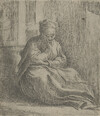
\includegraphics[keepaspectratio,width=0.6\textwidth]{thais-small.jpg}
  \captionart{MelancholieThais}
  \label{fig:thais}
\end{figure}

To see a fond mother, like \AE{}sop's ape, hug her child to death, a \authormarginnote{379}
\footnoteA{a man who knows of his wife's infidelity and puts up with it. \theeditor{}}{wittol} wink at his wife's honesty, and too perspicuous in all other
affairs; one stumble at a straw, and leap over a block; rob Peter, and
pay Paul; scrape unjust sums with one hand, purchase great manors by
corruption, fraud and cozenage, and liberally to distribute to the poor
with the other, give a remnant to pious uses, \etc{}. Penny wise, pound
foolish; blind men judge of colours; wise men silent, fools talk; \authormarginnote{380}
find fault with others, and do worse themselves; \authormarginnote{381}[5\baselineskip]denounce that in
public which he doth in secret; and which Aurelius Victor gives out of
Augustus, severely censure that in a third, of which he is most guilty
himself.

To see a poor fellow, or an hired servant venture his life for his new
master that will scarce give him his wages at year's end; A country
colon toil and moil, till and drudge for a prodigal idle drone, that
devours all the gain, or lasciviously consumes with fantastical
expenses; A noble man in a bravado to encounter death, and for a small
flash of honour to cast away himself; A worldling tremble at an
executor, and yet not fear hell-fire; To wish and hope for immortality,
desire to be happy, and yet by all means avoid death, a necessary
passage to bring him to it.

To see a foolhardy fellow like those old Danes, \li{qui decollari malunt
quam verberari}, die rather than be punished, in a sottish humour
embrace death with alacrity, yet \authormarginnote{382}[-3\baselineskip]scorn to lament his own sins and
miseries, or his clearest friends' departures.

To see wise men degraded, fools preferred, one govern towns and cities,
and yet a silly woman overrules him at home; \authormarginnote{383}Command a province,
and yet his own servants or children prescribe laws to him, as
Themistocles' son did in Greece; \authormarginnote{384}[2\baselineskip]What I will (said he) my mother
will, and what my mother will, my father doth.

To see horses ride in a coach, men draw it; dogs devour their masters; towers build masons;
children rule; old men go to school; women wear the breeches;
\authormarginnote{385}[\baselineskip]sheep demolish towns, devour men, \etc{}. And in a word, the world
turned upside downward. \li{O viveret Democritus}.\authormarginnote{386}[2\baselineskip] To insist in every particular were one of Hercules' labours,
there's so many ridiculous instances, as motes in the sun. \li{Quantum est
in rebus inane?} (How much vanity there is in things!) And who can speak
of all? \li{Crimine ab uno disce omnes}, take this for a taste.

But these are obvious to sense, trivial and well known, easy to be
discerned. How would Democritus have been moved, had he seen \authormarginnote{387}the
secrets of their hearts? If every man had a window in his breast, which
Momus would have had in Vulcan's man, or that which Tully so much
wished it were written in every man's forehead, \li{Quid quisque de
republica sentiret}, what he thought; or that it could be effected in an
instant, which Mercury did by Charon in Lucian, by touching of his
eyes, to make him discern \li{semel et simul rumores et susurros}.
%
\settowidth{\versewidth}{Spes hominum c\ae{}cas, morbos, votumque labores,}
\begin{verse}[\versewidth]
\textlatin{Spes hominum c\ae{}cas, morbos, votumque labores,}\\*
\textlatin{Et passim toto volitantes \ae{}there curas.}\\!
\end{verse}
\translationrule
\settowidth{\versewidth}{Blind hopes and wishes, their thoughts and affairs,}
\begin{verse}[\versewidth]
Blind hopes and wishes, their thoughts and affairs,\\*
Whispers and rumours, and those flying cares.\\!
\end{verse}

That he could \li{cubiculorum obductas foras recludere et secreta cordium
penetrare}, which Cyprian desired\authormarginnote{388}, open doors and locks, shoot
bolts, as Lucian's Gallus did with a feather of his tail: or Gyges'
invisible ring, or some rare perspective glass, or \emph{Otacousticon},
which would so multiply species, that a man might hear and see all at
once (as \authormarginnote{389} Martianus Capella's Jupiter did in a spear which he held
in his hand, which did present unto him all that was daily done upon
the face of the earth), observe cuckolds' horns, forgeries of
alchemists, the philosopher's stone, new projectors, \etc{}, and all those
works of darkness, foolish vows, hopes, fears and wishes, what a deal
of laughter would it have afforded? He should have seen windmills in
one man's head, an hornet's nest in another. Or had he been present
with Icaromenippus in Lucian at Jupiter's whispering place, \authormarginnote{390}and
heard one pray for rain, another for fair weather; one for his wife's,
another for his father's death, \etc{}; to ask that at God's hand which
they are abashed any man should hear: How would he have been
confounded? Would he, think you, or any man else, say that these men
were well in their wits? \li{H\ae{}c sani esse hominis quis sanus juret
Orestes?} Can all the hellebore in the Anticyr\ae{}\ cure these men? No,
sure, \authormarginnote{391}an acre of hellebore will not do it.

That which is more to be lamented, they are mad like \Seneca's blind
woman, and will not acknowledge, or \authormarginnote{392}seek for any cure of it, for
pauci vident morbum suum, omnes amant. If our leg or arm offend us, we
covet by all means possible to redress it; \authormarginnote{393}and if we labour of a
bodily disease, we send for a physician; but for the diseases of the
mind we take no notice of them: \authormarginnote{394}[\baselineskip]Lust harrows us on the one side;
envy, anger, ambition on the other. We are torn in pieces by our
passions, as so many wild horses, one in disposition, another in habit;
one is melancholy, another mad; \authormarginnote{395}[3\baselineskip]and which of us all seeks for
help, doth acknowledge his error, or knows he is sick? As that stupid
fellow put out the candle because the biting fleas should not find him;
he shrouds himself in an unknown habit, borrowed titles, because nobody
should discern him. Every man thinks with himself, \li{Egomet videor mihi
sanus}, I am well, I am wise, and laughs at others. And 'tis a general
fault amongst them all, that \authormarginnote{396}[3\baselineskip] which our forefathers have approved,
diet, apparel, opinions, humours, customs, manners, we deride and
reject in our time as absurd. Old men account juniors all fools, when
they are mere dizzards; and as to sailors, ---\li{terr\ae{}que urbesque
recedunt}--- they move, the land stands still, the world hath much more
wit, they dote themselves. Turks deride us, we them; Italians
Frenchmen, accounting them light headed fellows, the French scoff again
at Italians, and at their several customs; Greeks have condemned all
the world but themselves of barbarism, the world as much vilifies them
now; we account Germans heavy, dull fellows, explode many of their
fashions; they as contemptibly think of us; Spaniards laugh at all, and
all again at them. So are we fools and ridiculous, absurd in our
actions, carriages, diet, apparel, customs, and consultations; we \authormarginnote{397}
scoff and point one at another, when as in conclusion all are fools,
\authormarginnote{398} and they the veriest asses that hide their ears most. A private
man if he be resolved with himself, or set on an opinion, accounts all
idiots and asses that are not affected as he is, \authormarginnote{399}---\li{nil rectum,
nisi quod placuit sibi, ducit}, that are not so minded, \authormarginnote{400}(\li{quodque
volunt homines se bene velle putant}) all fools that think not as he
doth: he will not say with Atticus, \li{Suam quisque sponsam, mihi meam},
let every man enjoy his own spouse; but his alone is fair, \li{suus amor},
\etc{} and scorns all in respect of himself \authormarginnote{401}[-3\baselineskip]will imitate none, hear
none \authormarginnote{402}but himself, as \Pliny{} said, a law and example to himself. And
that which Hippocrates, in his epistle to Dionysius, reprehended of
old, is verified in our times, \li{Quisque in alio superfluum esse censet,
ipse quod non habet nec curat}, that which he hath not himself or doth
not esteem, he accounts superfluity, an idle quality, a mere foppery in
another: like \AE{}sop's fox, when he had lost his tail, would have all
his fellow foxes cut off theirs. The Chinese say, that we Europeans
have one eye, they themselves two, all the world else is blind: (though
\authormarginnote{403}Scaliger accounts them brutes too, \li{merum pecus}) so thou and thy
sectaries are only wise, others indifferent, the rest beside
themselves, mere idiots and asses. Thus not acknowledging our own
errors and imperfections, we securely deride others, as if we alone
were free, and spectators of the rest, accounting it an excellent
thing, as indeed it is, \li{Aliena optimum frui insania}, to make ourselves
merry with other men's obliquities, when as he himself is more faulty
than the rest, \li{mutato nomine, de te fabula narratur}, he may take
himself by the nose for a fool; and which one calls \li{maximum stultiti\ae{}}
specimen, to be ridiculous to others, and not to perceive or take
notice of it, as Marsyas was when he contended with Apollo, \li{non
intelligens se deridiculo haberi}, saith \Apuleius\authormarginnote{404}; 'tis his own
cause, he is a convicted madman, as \authormarginnote{405}\Austin{} well infers in the eyes
of wise men and angels he seems like one, that to our thinking walks
with his heels upwards. So thou laughest at me, and I at thee, both at
a third; and he returns that of the poet upon us again, \authormarginnote{406}[\baselineskip]\li{Hei mihi,
insanire me aiunt, quum ipsi ultro insaniant}. We accuse others of
madness, of folly, and are the veriest dizzards ourselves. For it is a
great sign and property of a fool (which Eccl. \rn{x.} 3, points at) out of
pride and self-conceit to insult, vilify, condemn, censure, and call
other men fools (\li{Non videmus mantic\ae{}\ quod a tergo est}) to tax that in
others of which we are most faulty; teach that which we follow not
ourselves: For an inconstant man to write of constancy, a profane liver
prescribe rules of sanctity and piety, a dizzard himself make a
treatise of wisdom, or with Sallust to rail downright at spoilers of
countries, and yet in \authormarginnote{407}office to be a most grievous poller himself.

This argues weakness, and is an evident sign of such parties'
indiscretion. \authormarginnote{408}\li{Peccat uter nostrum cruce dignius?} Who is the fool
now? Or else peradventure in some places we are all mad for company,
and so 'tis not seen, \li{Satietas erroris et dementi\ae{}, pariter
absurditatem et admirationem tollit.} 'Tis with us, as it was of old (in
\authormarginnote{409}Tully's censure at least) with C. Pimbria in Rome, a bold,
hair-brain, mad fellow, and so esteemed of all, such only excepted,
that were as mad as himself: now in such a case there is \authormarginnote{410}no notice
taken of it.
%
\settowidth{\versewidth}{Maxima pars hominum morbo jactatur eodem.}
\begin{verse}[\versewidth]
\textlatin{Nimirum insanus paucis videatur; eo quod}\\*
\textlatin{Maxima pars hominum morbo jactatur eodem.}
\end{verse}
\translationrule
\settowidth{\versewidth}{When all are mad, where all are like opprest}
\begin{verse}[\versewidth]
When all are mad, where all are like opprest\\*
Who can discern one mad man from the rest?\\!
\end{verse}

But put case they do perceive it, and some one be manifestly convicted
of madness, \authormarginnote{411}he now takes notice of his folly, be it in action,
gesture, speech, a vain humour he hath in building, bragging, jangling,
spending, gaming, courting, scribbling, prating, for which he is
ridiculous to others, \authormarginnote{412}on which he dotes, he doth acknowledge as
much: yet with all the rhetoric thou hast, thou canst not so recall
him, but to the contrary notwithstanding, he will persevere in his
dotage. 'Tis \li{amabilis insania, et mentis gratissimus error}, so
pleasing, so delicious, that he cannot leave it\authormarginnote{413}. He knows his
error, but will not seek to decline it, tell him what the event will
be, beggary, sorrow, sickness, disgrace, shame, loss, madness, yet
\authormarginnote{414}an angry man will prefer vengeance, a lascivious his whore, a
thief his booty, a glutton his belly, before his welfare. Tell an
epicure, a covetous man, an ambitious man of his irregular course, wean
him from it a little, \li{pol me occidistis amici}, he cries anon, you have
undone him, and as \authormarginnote{415}a dog to his vomit, he returns to it again; no
persuasion will take place, no counsel, say what thou canst,
%
\begin{verse}
\textlatin{Clames licet et mare coelo}\\*
---\textlatin{Confundas, surdo narras,}\authorlatintrans{416}
\end{verse}

demonstrate as Ulysses did to \authormarginnote{417}Elpenor and Gryllus, and the rest of
his companions those swinish men, he is irrefragable in his humour, he
will be a hog still; bray him in a mortar, he will be the same. If he
be in an heresy, or some perverse opinion, settled as some of our
ignorant Papists are, convince his understanding, show him the several
follies and absurd fopperies of that sect, force him to say, veris
vincor, make it as clear as the sun, \authormarginnote{418}[-1\baselineskip]he will err still, peevish
and obstinate as he is; and as he said \authormarginnote{419}\li{si in hoc erro, libenter
erro, nec hunc errorem auferri mihi volo}; I will do as I have done, as
my predecessors have done, \authormarginnote{420}[-1\baselineskip]and as my friends now do: I will dote
for company. Say now, are these men \authormarginnote{421}mad or no, \authormarginnote{422}[2\baselineskip]\li{Heus age
responde?} are they ridiculous? \li{cedo quemvis arbitrum}, are they \li{san\ae{}
mentis}, sober, wise, and discreet? have they common sense? ---\authormarginnote{423}\li{uter
est insanior horum?} I am of Democritus' opinion for my part, I hold
them worthy to be laughed at; a company of brain-sick dizzards, as mad
as \authormarginnote{424}Orestes and Athamas, that they may go ride the ass, and all
sail along to the Anticyr\ae{}, in the ship of fools for company together.

I need not much labour to prove this which I say otherwise than thus,
make any solemn protestation, or swear, I think you will believe me
without an oath; say at a word, are they fools? I refer it to you,
though you be likewise fools and madmen yourselves, and I as mad to ask
the question; for what said our comical Mercury?
%
\begin{verse}
\textlatin{Justum ab injustis petere insipientia est.}\authormarginnote{425}
\end{verse}
\translationrule
\begin{verse}
I'll stand to your censure yet, what think you?
\end{verse}

But forasmuch as I undertook at first, that kingdoms, provinces,
families, were melancholy as well as private men, I will examine them
in particular, and that which I have hitherto dilated at random, in
more general terms, I will particularly insist in, prove with more
special and evident arguments, testimonies, illustrations, and that in
brief. \authormarginnote{426}\li{Nunc accipe quare desipiant omnes \ae{}que ac tu.} My first
argument is borrowed from Solomon, an arrow drawn out of his
sententious quiver, Pro. \rn{iii.} 7, Be not wise in thine own eyes. And
\rn{xxvi.} 12, Seest thou a man wise in his own conceit? more hope is of a
fool than of him. Isaiah pronounceth a woe against such men, cap. v.
21, that are wise in their own eyes, and prudent in their own sight.

For hence we may gather, that it is a great offence, and men are much
deceived that think too well of themselves, an especial argument to
convince them of folly. Many men (saith \authormarginnote{427}\Seneca) had been without
question wise, had they not had an opinion that they had attained to
perfection of knowledge already, even before they had gone half way,
too forward, too ripe, pr\ae{}properi, too quick and ready, \authormarginnote{428}\li{cito
prudentes, cito pii, cito mariti, cito patres, cito sacerdotes, cito
omnis officii capaces et curiosi}, they had too good a conceit of
themselves, and that marred all; of their worth, valour, skill, art,
learning, judgment, eloquence, their good parts; all their geese are
swans, and that manifestly proves them to be no better than fools. In
former times they had but seven wise men, now you can scarce find so
many fools. Thales sent the golden tripos, which the fishermen found,
and the oracle commanded to be \authormarginnote{429} given to the wisest, to Bias, Bias
to Solon, \etc{}. If such a thing were now found, we should all fight for
it, as the three goddesses did for the golden apple, we are so wise: we
have women politicians, children metaphysicians; every silly fellow can
square a circle, make perpetual motions, find the philosopher's stone,
interpret Apocalypses, make new Theories, a new system of the world,
new Logic, new Philosophy, \etc{}. \li{Nostra utique regio}, saith
\authormarginnote{430}Petronius, our country is so full of deified spirits, divine
souls, that you may sooner find a God than a man amongst us, we think
so well of ourselves, and that is an ample testimony of much folly.

My second argument is grounded upon the like place of Scripture, which
though before mentioned in effect, yet for some reasons is to be
repeated (and by Plato's good leave, I may do it, \textgreek{δίς τὸ καλὸν
ρηθέν ὀυδέν βλάπτει}\authormarginnote{431}) Fools (saith David) by reason of their
transgressions. \etc{}. Psal. \rn{cvii.} 17. Hence Musculus infers all
transgressors must needs be fools. So we read Rom. \rn{ii.}, Tribulation and
anguish on the soul of every man that doeth evil; but all do evil. And
Isaiah, \rn{lxv.} 14, My servant shall sing for joy, and \authormarginnote{432}ye shall cry
for sorrow of heart, and vexation of mind. 'Tis ratified by the common
consent of all philosophers. Dishonesty (saith Cardan) is nothing else
but folly and madness. \li{Probus quis nobiscum vivit?}\authorlatintrans{433.5}\authormarginnote{433} Show me an
honest man, \li{Nemo malus qui non stultus}, 'tis Fabius' aphorism to the
same end. If none honest, none wise, then all fools. And well may they
be so accounted: for who will account him otherwise, \li{Qui iter adornat
in occidentem, quum properaret in orientem?} that goes backward all his
life, westward, when he is bound to the east? or hold him a wise man
(saith \authormarginnote{434}Musculus) that prefers momentary pleasures to eternity,
that spends his master's goods in his absence, forthwith to be
condemned for it? \li{Nequicquam sapit qui sibi non sapit}, who will say
that a sick man is wise, that eats and drinks to overthrow the
temperature of his body? Can you account him wise or discreet that
would willingly have his health, and yet will do nothing that should
procure or continue it? \authormarginnote{435}Theodoret, out of Plotinus the Platonist,
holds it a ridiculous thing for a man to live after his own laws, to do
that which is offensive to God, and yet to hope that he should save
him: and when he voluntarily neglects his own safety, and contemns the
means, to think to be delivered by another: who will say these men are
wise?

A third argument may be derived from the precedent, \authormarginnote{436}all men are
carried away with passion, discontent, lust, pleasures, \etc{}, they
generally hate those virtues they should love, and love such vices they
should hate. Therefore more than melancholy, quite mad, brute beasts,
and void of reason, so \Chrysostom{} contends; or rather dead and buried
alive, as \authormarginnote{437} Philo Judeus concludes it for a certainty, of all such
that are carried away with passions, or labour of any disease of the
mind. Where is fear and sorrow, there \authormarginnote{438}Lactantius stiffly
maintains, wisdom cannot dwell,
%
\begin{verse}
---\textlatin{qui cupiet, metuet quoque porro,}\\*
\textlatin{Qui metuens vivit, liber mihi non erit unquam.}\authorlatintrans{439}
\end{verse}

\Seneca and the rest of the stoics are of opinion, that where is any the
least perturbation, wisdom may not be found. What more ridiculous, as
\authormarginnote{440}[-2\baselineskip]Lactantius urges, than to hear how Xerxes whipped the Hellespont,
threatened the Mountain Athos, and the like. To speak \li{ad rem}, who is
free from passion? \authormarginnote{441}[-2\baselineskip]\li{Mortalis nemo est quem non attingat dolor, morbusve}, as \authormarginnote{442}Tully determines out of an old poem, no mortal men
can avoid sorrow and sickness, and sorrow is an inseparable companion
from melancholy. \authormarginnote{443}\Chrysostom{} pleads farther yet, that they are more
than mad, very beasts, stupefied and void of common sense: For how
(saith he) shall I know thee to be a man, when thou kickest like an
ass, neighest like a horse after women, ravest in lust like a bull,
ravenest like a bear, stingest like a scorpion, rakest like a wolf, as
subtle as a fox, as impudent as a dog? Shall I say thou art a man, that
hast all the symptoms of a beast? How shall I know thee to be a man? by
thy shape? That affrights me more, when I see a beast in likeness of a
man.

\authormarginnote{444}\Seneca calls that of Epicurus, \li{magnificam vocem}, an heroical
speech, A fool still begins to live, and accounts it a filthy lightness
in men, every day to lay new foundations of their life, but who doth
otherwise? One travels, another builds; one for this, another for that
business, and old folks are as far out as the rest; \li{O dementem
senectutem}, Tully exclaims. Therefore young, old, middle age, are all
stupid, and dote.

\authormarginnote{445}\AE{}neas Sylvius, amongst many other, sets down three special ways
to find a fool by. He is a fool that seeks that he cannot find: he is a
fool that seeks that, which being found will do him more harm than
good: he is a fool, that having variety of ways to bring him to his
journey's end, takes that which is worst. If so, methinks most men are
fools; examine their courses, and you shall soon perceive what dizzards
and mad men the major part are.

Beroaldus will have drunkards, afternoon men, and such as more than
ordinarily delight in drink, to be mad. The first pot quencheth thirst,
so Panyasis the poet determines in Athen\ae{}us, \li{secunda gratiis, horis et
Dyonisio}: the second makes merry, the third for pleasure, quarta, ad
insaniam, the fourth makes them mad. If this position be true, what a
catalogue of mad men shall we have? what shall they be that drink four
times four? \li{Nonne supra omnem furorem, supra omnem insanian reddunt
insanissimos?} I am of his opinion, they are more than mad, much worse
than mad.

The \authormarginnote{446}Abderites condemned Democritus for a mad man, because he was
sometimes sad, and sometimes again profusely merry. \li{Hac Patria} (saith
Hippocrates) \li{ob risum furere et insanire dicunt}, his countrymen hold
him mad because he laughs; \authormarginnote{447}and therefore he desires him to advise
all his friends at Rhodes, that they do not laugh too much, or be over
sad. Had those Abderites been conversant with us, and but seen what
\authormarginnote{448} fleering and grinning there is in this age, they would certainly
have concluded, we had been all out of our wits.

Aristotle in his Ethics holds \li{felix idemque sapiens}, to be wise and
happy, are reciprocal terms, \li{bonus idemque sapiens honestus}. 'Tis \authormarginnote{449}
Tully's paradox, wise men are free, but fools are slaves, liberty is a
power to live according to his own laws, as we will ourselves: who hath
this liberty? who is free?
%
\settowidth{\versewidth}{Quem neque pauperis, neque mors, neque vincula terrent,}
\begin{verse}[\versewidth]
---\textlatin{sapiens sibique imperiosus,}\\*
\textlatin{Quem neque pauperis, neque mors, neque vincula terrent,}\\*
\textlatin{Responsare cupidinibus, contemnere honores}\\*
\textlatin{Fortis, et in seipso totus teres atque rotundus.}\authormarginnote{450}\\!
\end{verse}
\translationrule
\settowidth{\versewidth}{Checks his desires, scorns honours, just and right.}
\begin{verse}[\versewidth]
He is wise that can command his own will,\\*
Valiant and constant to himself still,\\*
Whom poverty nor death, nor bands can fright,\\*
Checks his desires, scorns honours, just and right.\\!
\end{verse}

But where shall such a man be found? If no where, then \li{e diametro}, we
are all slaves, senseless, or worse. \li{Nemo malus felix}. But no man is
happy in this life, none good, therefore no man wise. \li{Rari quippe
boni}\authorlatintrans{451.5}\authormarginnote{451}--- For one virtue you shall find ten vices in the same party;
\li{pauci Promethei, multi Epimethei}. We may peradventure usurp the name,
or attribute it to others for favour, as Carolus Sapiens, Philippus
Bonus, Lodovicus Pius, \etc{}, and describe the properties of a wise man,
as Tully doth an orator, Xenophon Cyrus, Castilio a courtier, Galen
temperament, an aristocracy is described by politicians. But where
shall such a man be found?
%
\settowidth{\versewidth}{Vir bonus et sapiens, qualem vix repperit unum}
\begin{verse}[\versewidth]
\textlatin{Vir bonus et sapiens, qualem vix repperit unum}\\*
\textlatin{Millibus e multis hominum consultus Apollo.}\\!
\end{verse}
\translationrule
\begin{verse}
A wise, a good man in a million,\\*
Apollo consulted could scarce find one.\\!
\end{verse}

A man is a miracle of himself, but Trismegistus adds, \li{Maximum miraculum
homo sapiens}, a wise man is a wonder: \li{multi Thirsigeri, pauci Bacchi}.

Alexander when he was presented with that rich and costly casket of
king Darius, and every man advised him what to put in it, he reserved
it to keep Homer's works, as the most precious jewel of human wit, and
yet \authormarginnote{452} Scaliger upbraids Homer's muse, \li{Nutricem insan\ae{}\ sapienti\ae{}},
a nursery of madness, \authormarginnote{453}impudent as a court lady, that blushes at
nothing. Jacobus Mycillus, Gilbertus Cognatus, Erasmus, and almost all
posterity admire Lucian's luxuriant wit, yet Scaliger rejects him in
his censure, and calls him the Cerberus of the muses. Socrates, whom
all the world so much magnified, is by Lactantius and Theodoret
condemned for a fool. \idxname{Plutarch} extols \Seneca's wit beyond all the
Greeks, \li{nulli secundus}, yet \authormarginnote{454} \Seneca saith of himself, when I would
solace myself with a fool, I reflect upon myself, and there I have him.

Cardan, in his Sixteenth Book of Subtleties, reckons up twelve
supereminent, acute philosophers, for worth, subtlety, and wisdom:
Archimedes, Galen, Vitruvius, Architas Tarentinus, Euclid, Geber, that
first inventor of Algebra, Alkindus the Mathematician, both Arabians,
with others. But his \li{triumviri terrarum} far beyond the rest, are
Ptolom\ae{}us, Plotinus, Hippocrates. Scaliger \li{exercitat. 224}, scoffs at
this censure of his, calls some of them carpenters and mechanicians, he
makes Galen \li{fimbriam Hippocratis}, a skirt of Hippocrates: and the said
\authormarginnote{455}Cardan himself elsewhere condemns both Galen and Hippocrates for
tediousness, obscurity, confusion. Paracelsus will have them both mere
idiots, infants in physic and philosophy. Scaliger and Cardan admire
Suisset the Calculator, \li{qui pene modum excessit humani ingenii}, and yet
\authormarginnote{456}Lod. Vives calls them nugas Suisseticas: and Cardan, opposite to
himself in another place, contemns those ancients in respect of times
present, \authormarginnote{457}\li{Majoresque nostros ad presentes collatos juste pueros
appellari}. In conclusion, the said \authormarginnote{458}Cardan and Saint Bernard will
admit none into this catalogue of wise men, \authormarginnote{459}but only prophets and
apostles; how they esteem themselves, you have heard before. We are
worldly-wise, admire ourselves, and seek for applause: but hear Saint
\authormarginnote{460}[2\baselineskip]Bernard, \li{quanto magis foras es sapiens, tanto magis intus stultus efficeris, \etc{} in omnibus es prudens, circa teipsum insipiens}: the more
wise thou art to others, the more fool to thyself. I may not deny but
that there is some folly approved, a divine fury, a holy madness, even
a spiritual drunkenness in the saints of God themselves; \li{sanctum
insanium} Bernard calls it (though not as blaspheming \authormarginnote{461}Vorstius,
would infer it as a passion incident to God himself, but) familiar to
good men, as that of Paul, 2 Cor. he was a fool, \etc{} and Rom. \rn{ix.} he
wisheth himself to be anathematised for them. Such is that drunkenness
which Ficinus speaks of, when the soul is elevated and ravished with a
divine taste of that heavenly nectar, which poets deciphered by the
sacrifice of Dionysius, and in this sense with the poet, \authormarginnote{462}\li{insanire
lubet}, as \Austin{} exhorts us, \li{ad ebrietatem se quisque paret}, let's all
be mad and \authormarginnote{463}drunk. But we commonly mistake, and go beyond our
commission, we reel to the opposite part, \authormarginnote{464}[\baselineskip]we are not capable of
it, \authormarginnote{465}[2\baselineskip]and as he said of the Greeks, \li{Vos Gr\ae{}ci semper pueri, vos Britanni, Galli, Germani, Itali, \etc{}} you are a company of fools.

Proceed now a \li{partibus ad totum}, or from the whole to parts, and you
shall find no other issue, the parts shall be sufficiently dilated in
this following Preface. The whole must needs follow by a sorites or
induction. Every multitude is mad, \authormarginnote{466}\li{bellua multorum capitum}, (a
many-headed beast), precipitate and rash without judgment, \li{stultum
animal}, a roaring rout. \authormarginnote{467}Roger Bacon proves it out of Aristotle,
\li{Vulgus dividi in oppositum contra sapientes, quod vulgo videtur verum,
falsum est}; that which the commonalty accounts true, is most part
false, they are still opposite to wise men, but all the world is of
this humour (vulgus), and thou thyself art \li{de vulgo}, one of the
commonalty; and he, and he, and so are all the rest; and therefore, as
Phocion concludes, to be approved in nought you say or do, mere idiots
and asses. Begin then where you will, go backward or forward, choose
out of the whole pack, wink and choose, you shall find them all alike,
never a barrel better herring.

Copernicus, Atlas his successor, is of opinion, the earth is a planet,
moves and shines to others, as the moon doth to us. Digges, Gilbert,
Keplerus, Origanus, and others, defend this hypothesis of his in sober
sadness, and that the moon is inhabited: if it be so that the earth is
a moon, then are we also giddy, vertiginous and lunatic within this
sublunary maze.

I could produce such arguments till dark night: if you should hear the
rest,
%
\begin{verse}
\textlatin{Ante diem clauso component vesper Olimpo:}
\end{verse}
\translationrule
\begin{verse}
Through such a train of words if I should run,\\*
The day would sooner than the tale be done:
\end{verse}

but according to my promise, I will descend to particulars. This
melancholy extends itself not to men only, but even to vegetals and
sensibles. I speak not of those creatures which are saturnine,
melancholy by nature, as lead, and such like minerals, or those plants,
rue, cypress, \etc{} and hellebore itself, of which \authormarginnote{468}Agrippa treats,
fishes, birds, and beasts, hares, conies, dormice, \etc{}, owls, bats,
nightbirds, but that artificial, which is perceived in them all. Remove
a plant, it will pine away, which is especially perceived in date
trees, as you may read at large in Constantine's husbandry, that
antipathy betwixt the vine and the cabbage, vine and oil. Put a bird in
a cage, he will die for sullenness, or a beast in a pen, or take his
young ones or companions from him, and see what effect it will cause.

But who perceives not these common passions of sensible creatures,
fear, sorrow, \etc{}. Of all other, dogs are most subject to this malady,
insomuch some hold they dream as men do, and through violence of
melancholy run mad; I could relate many stories of dogs that have died
for grief, and pined away for loss of their masters, but they are
common in every \authormarginnote{469}author.

Kingdoms, provinces, and politic bodies are likewise sensible and
subject to this disease, as \authormarginnote{470}Boterus in his politics hath proved at
large. As in human bodies (saith he) there be diverse alterations
proceeding from humours, so be there many diseases in a commonwealth,
which do as diversely happen from several distempers, as you may easily
perceive by their particular symptoms. For where you shall see the
people civil, obedient to God and princes, judicious, peaceable and
quiet, rich, fortunate, \authormarginnote{471}and flourish, to live in peace, in unity
and concord, a country well tilled, many fair built and populous
cities, \li{ubi incol\ae{}\ nitent} as old Cato said\authormarginnote{472}, the people are neat,
polite and terse, \li{ubi bene, beateque vivunt}, which our politicians make
the chief end of a commonwealth; and which \authormarginnote{473} Aristotle, Polit. lib.
3, cap. 4, calls \li{Commune bonum}, Polybius lib. 6, \li{optabilem et selectum
statum}, that country is free from melancholy; as it was in Italy in the
time of Augustus, now in China, now in many other flourishing kingdoms
of Europe. But whereas you shall see many discontents, common
grievances, complaints, poverty, barbarism, beggary, plagues, wars,
rebellions, seditions, mutinies, contentions, idleness, riot,
epicurism, the land lie untilled, waste, full of bogs, fens, deserts,
\etc{}, cities decayed, base and poor towns, villages depopulated, the
people squalid, ugly, uncivil; that kingdom, that country, must needs
be discontent, melancholy, hath a sick body, and had need to be
reformed.

Now that cannot well be effected, till the causes of these maladies be
first removed, which commonly proceed from their own default, or some
accidental inconvenience: as to be situated in a bad clime, too far
north, sterile, in a barren place, as the desert of Libya, deserts of
Arabia, places void of waters, as those of Lop and Belgian in Asia, or
in a bad air, as at Alexandretta, Bantam, Pisa, Durrazzo, S. John de
Ulloa, \etc{}, or in danger of the sea's continual inundations, as in many
places of the Low Countries and elsewhere, or near some bad neighbours,
as Hungarians to Turks, Podolians to Tartars, or almost any bordering
countries, they live in fear still, and by reason of hostile incursions
are oftentimes left desolate. So are cities by reason \authormarginnote{474}of wars,
fires, plagues, inundations, \authormarginnote{475}[2\baselineskip]wild beasts, decay of trades, barred
havens, the sea's violence, as Antwerp may witness of late, Syracuse of
old, Brundusium in Italy, Rye and Dover with us, and many that at this
day suspect the sea's fury and rage, and labour against it as the
Venetians to their inestimable charge. But the most frequent maladies
are such as proceed from themselves, as first when religion and God's
service is neglected, innovated or altered, where they do not fear God,
obey their prince, where atheism, epicurism, sacrilege, simony, \etc{},
and all such impieties are freely committed, that country cannot
prosper. When Abraham came to Gerar, and saw a bad land, he said, sure
the fear of God was not in that place. \authormarginnote{476} Cyprian Echovius, a
Spanish chorographer, above all other cities of Spain, commends
Borcino, in which there was no beggar, no man poor, \etc{}, but all rich,
and in good estate, and he gives the reason, because they were more
religious than, their neighbours: why was Israel so often spoiled by
their enemies, led into captivity, \etc{}, but for their idolatry, neglect
of God's word, for sacrilege, even for one Achan's fault? And what
shall we except that have such multitudes of Achans, church robbers,
simoniacal patrons, \etc{}, how can they hope to flourish, that neglect
divine duties, that live most part like Epicures?
Other common grievances are generally noxious to a body politic;
alteration of laws and customs, breaking privileges, general
oppressions, seditions, \etc{}, observed by \authormarginnote{477}Aristotle, Bodin,
Boterus, Junius, Arniscus, \etc{}. I will only point at some of chiefest.

\authormarginnote{478}\li{Impotentia gubernandi}, ataxia, confusion, ill government, which
proceeds from unskilful, slothful, griping, covetous, unjust, rash, or
tyrannizing magistrates, when they are fools, idiots, children, proud,
wilful, partial, indiscreet, oppressors, giddy heads, tyrants, not able
or unfit to manage such offices: \authormarginnote{479}many noble cities and flourishing
kingdoms by that means are desolate, the whole body groans under such
heads, and all the members must needs be disaffected, as at this day
those goodly provinces in Asia Minor, \etc{} groan under the burthen of a
Turkish government; and those vast kingdoms of Muscovia, Russia,
\authormarginnote{480}under a tyrannizing duke. Who ever heard of more civil and rich
populous countries than those of Greece, Asia Minor, abounding with all
\authormarginnote{481}wealth, multitudes of inhabitants, force, power, splendour and
magnificence? and that miracle of countries, \authormarginnote{482}the Holy Land, that
in so small a compass of ground could maintain so many towns, cities,
produce so many fighting men? Egypt another paradise, now barbarous and
desert, and almost waste, by the despotical government of an imperious
Turk, \li{intolerabili servitutis jugo premitur} (\authormarginnote{483}one saith) not only
fire and water, goods or lands, \li{sed ipse spiritus ab insolentissimi
victoris pendet nutu}, such is their slavery, their lives and souls
depend upon his insolent will and command. A tyrant that spoils all
wheresoever he comes, insomuch that an \authormarginnote{484}historian complains, if an
old inhabitant should now see them, he would not know them, if a
traveller, or stranger, it would grieve his heart to behold them.

Whereas Aristotle notes\authormarginnote{485}, \li{Nov\ae{}\ exactiones, nova onera imposita},
new burdens and exactions daily come upon them, like those of which
Zosimus, lib. 2, so grievous, \li{ut viri uxores, patres filios
prostituerent ut exactoribus e questu, \etc{}}, they must needs be
discontent, \li{hinc civitatum gemitus et ploratus}, as \authormarginnote{486} Tully holds,
hence come those complaints and tears of cities, poor, miserable,
rebellious, and desperate subjects, as \authormarginnote{487}[-1\baselineskip]Hippolitus adds; and
\authormarginnote{488}[\baselineskip]as a judicious countryman of ours observed not long since, in a
survey of that great Duchy of Tuscany, the people lived much grieved
and discontent, as appeared by their manifold and manifest complainings
in that kind. That the state was like a sick body which had lately
taken physic, whose humours are not yet well settled, and weakened so
much by purging, that nothing was left but melancholy.

Whereas the princes and potentates are immoderate in lust, hypocrites,
epicures, of no religion, but in show: \li{Quid hypocrisi fragilius?} what
so brittle and unsure? what sooner subverts their estates than
wandering and raging lusts, on their subjects' wives, daughters? to say
no worse. That they should \li{facem pr\ae{}ferre}, lead the way to all
virtuous actions, are the ringleaders oftentimes of all mischief and
dissolute courses, and by that means their countries are plagued,
\authormarginnote{489}and they themselves often ruined, banished, or murdered by
conspiracy of their subjects, as Sardanapalus was, Dionysius Junior,
Heliogabalus, Periander, Pisistratus, Tarquinius, Timocrates,
Childericus, Appius Claudius, Andronicus, Galeacius Sforza, Alexander
Medices, \etc{}.

Whereas the princes or great men are malicious, envious, factious,
ambitious, emulators, they tear a commonwealth asunder, as so many
Guelfs and Gibelines disturb the quietness of it, \authormarginnote{490}and with mutual
murders let it bleed to death; our histories are too full of such
barbarous inhumanities, and the miseries that issue from them.

Whereas they be like so many horseleeches, hungry, griping, corrupt,
\authormarginnote{491} covetous, \li{avaritice mancipia}, ravenous as wolves, for as Tully
writes: \li{qui pr\ae{}est prodest, et qui pecudibus pr\ae{}est, debet eorum
utilitati inservire}: or such as prefer their private before the public
good. For as \authormarginnote{492}[-1\baselineskip]he said long since, \li{res privat\ae{}\ publicis semper officere}. Or whereas they be illiterate, ignorant, empirics in policy,
\li{ubi deest facultas}, \authormarginnote{493}[-2\baselineskip]\li{virtus} (Aristot. pol. 5, cap. 8.) \li{et scientia},
wise only by inheritance, and in authority by birthright, favour, or
for their wealth and titles; there must needs be a fault, \authormarginnote{494}[2\baselineskip]a great
defect: because as an \authormarginnote{495}[5\baselineskip]old philosopher affirms, such men are not
always fit. Of an infinite number, few alone are senators, and of those
few, fewer good, and of that small number of honest, good, and noble
men, few that are learned, wise, discreet and sufficient, able to
discharge such places, it must needs turn to the confusion of a state.

For as the \authormarginnote{496}Princes are, so are the people; \li{Qualis Rex, talis grex}:
and which \authormarginnote{497}[5\baselineskip]Antigonus right well said of old, \li{qui Macedonia regem
erudit, omnes etiam subditos erudit}, he that teacheth the king of
Macedon, teacheth all his subjects, is a true saying still.
%
\begin{verse}
For Princes are the glass, the school, the book,\\*
Where subjects' eyes do learn, do read, do look.
\end{verse}

\begin{verse}
---\textlatin{Velocius et citius nos}\\*
\textlatin{Corrumpunt vitiorum exempla domestica, magnis}\\*
\textlatin{Cum subeant animos auctoribus.}---\authorlatintrans{498}
\end{verse}

Their examples are soonest followed, vices entertained, if they be
profane, irreligious, lascivious, riotous, epicures, factious,
covetous, ambitious, illiterate, so will the commons most part be,
idle, unthrifts, prone to lust, drunkards, and therefore poor and needy
(\inlinegreek{ἡ πενια στάσιν ἐμποιει καὶ κακουργίαν}, for poverty begets sedition and
villainy) upon all occasions ready to mutiny and rebel, discontent
still, complaining, murmuring, grudging, apt to all outrages, thefts,
treasons, murders, innovations, in debt, shifters, cozeners, outlaws,
\li{Profligat\ae{}\ fam\ae{}\ ac vit\ae{}}. It was an old \authormarginnote{499}politician's aphorism,
They that are poor and bad envy rich, hate good men, abhor the present
government, wish for a new, and would have all turned topsy-turvy. When
Catiline rebelled in Rome, he got a company of such debauched rogues
together, they were his familiars and coadjutors, and such have been
your rebels most part in all ages, Jack Cade, Tom Straw, Kette, and his
companions.

Where they be generally riotous and contentious, where there be many
discords, many laws, many lawsuits, many lawyers and many physicians,
it is a manifest sign of a distempered, melancholy state, as \authormarginnote{500}Plato
long since maintained: for where such kind of men swarm, they will make
more work for themselves, and that body politic diseased, which was
otherwise sound. A general mischief in these our times, an insensible
plague, and never so many of them: which are now multiplied (saith Mat.
Geraldus, \authormarginnote{501}a lawyer himself) as so many locusts, not the parents,
but the plagues of the country, and for the most part a supercilious,
bad, covetous, litigious generation of men. \authormarginnote{502}Crumenimulga natio \etc{}.

A purse-milking nation, a clamorous company, gowned vultures, \authormarginnote{503}\li{qui
ex injuria vivent et sanguine civium, thieves and seminaries of
discord}; worse than any pollers by the highway side, \li{auri accipitres,
auri exterebronides, pecuniarum hamiol\ae{}, quadruplatores, curi\ae{}
harpagones, fori tintinabula, monstra hominum, mangones, \etc{}} that take
upon them to make peace, but are indeed the very disturbers of our
peace, a company of irreligious harpies, scraping, griping catchpoles,
(I mean our common hungry pettifoggers, \authormarginnote{504}\li{rabulas forenses}, love and
honour in the meantime all good laws, and worthy lawyers, that are so
many \authormarginnote{505}oracles and pilots of a well-governed commonwealth). Without
art, without judgment, that do more harm, as \authormarginnote{506}Livy said, \li{quam bella
externa, fames, morbive}, than sickness, wars, hunger, diseases; and
cause a most incredible destruction of a commonwealth, saith
\authormarginnote{507}Sesellius, a famous civilian sometimes in Paris, as ivy doth by an
oak, embrace it so long, until it hath got the heart out of it, so do
they by such places they inhabit; no counsel at all, no justice, no
speech to be had, \li{nisi eum premulseris}, he must be fed still, or else
he is as mute as a fish, better open an oyster without a knife. \li{Experto
crede} (saith \authormarginnote{508} Salisburiensis) \li{in manus eorum millies incidi, et
Charon immitis qui nulli pepercit unquam, his longe clementior est}; I
speak out of experience, I have been a thousand times amongst them, and
Charon himself is more gentle than they; \authormarginnote{509}he is contented with his
single pay, but they multiply still, they are never satisfied, besides
they have \li{damnificas linguas}, as he terms it, \li{nisi funibus argenteis
vincias}, they must be fed to say nothing, and \authormarginnote{510}get more to hold
their peace than we can to say our best. They will speak their clients
fair, and invite them to their tables, but as he follows it, \authormarginnote{511}of
all injustice there is none so pernicious as that of theirs, which when
they deceive most, will seem to be honest men. They take upon them to
be peacemakers, \li{et fovere causas humilium}, to help them to their right,
\li{patrocinantur afflictis}, \authormarginnote{512}but all is for their own good, \li{ut loculos
pleniorom exhauriant}, they plead for poor men gratis, but they are but
as a stale to catch others. If there be no jar, \authormarginnote{513}they can make a
jar, out of the law itself find still some quirk or other, to set them
at odds, and continue causes so long, \li{lustra aliquot}, I know not how
many years before the cause is heard, and when 'tis judged and
determined by reason of some tricks and errors, it is as fresh to
begin, after twice seven years sometimes, as it was at first; and so
they prolong time, delay suits till they have enriched themselves, and
beggared their clients. And, as \authormarginnote{514}Cato inveighed against Isocrates'
scholars, we may justly tax our wrangling lawyers, they do consenescere
\li{in litibus}, are so litigious and busy here on earth, that I think they
will plead their client's causes hereafter, some of them in hell. \authormarginnote{515}
Simlerus complains amongst the Swissers of the advocates in his time,
that when they should make an end, they began controversies, and
protract their causes many years, persuading them their title is good,
till their patrimonies be consumed, and that they have spent more in
seeking than the thing is worth, or they shall get by the recovery. So
that he that goes to law, as the proverb is, \authormarginnote{516}holds a wolf by the
ears, or as a sheep in a storm runs for shelter to a brier, if he
prosecute his cause he is consumed, if he surcease his suit he loseth
all; \authormarginnote{517}what difference? They had wont heretofore, saith \Austin{}, to
end matters, \li{per communes arbitros}; and so in Switzerland (we are
informed by \authormarginnote{518}Simlerus), they had some common arbitrators or daysmen
in every town, that made a friendly composition betwixt man and man,
and he much wonders at their honest simplicity, that could keep peace
so well, and end such great causes by that means. At \authormarginnote{519}[\baselineskip]Fez in
Africa, they have neither lawyers nor advocates; but if there be any
controversies amongst them, both parties plaintiff and defendant come
to their Alfakins or chief judge, and at once without any farther
appeals or pitiful delays, the cause is heard and ended. Our
forefathers, as \authormarginnote{520}[\baselineskip]a worthy chorographer of ours observes, had wont
\li{pauculis cruculis aureis}, with a few golden crosses, and lines in
verse, make all conveyances, assurances. And such was the candour and
integrity of succeeding ages, that a deed (as I have oft seen) to
convey a whole manor, was implicite contained in some twenty lines or
thereabouts; like that scede or Sytala Laconica, so much renowned of
old in all contracts, which \authormarginnote{521}Tully so earnestly commends to
Atticus, \idxname{Plutarch} in his Lysander, Aristotle polit.: Thucydides, lib.
1, \authormarginnote{522}Diodorus and Suidus approve and magnify, for that laconic
brevity in this kind; and well they might, for, according to
Tertullian\authormarginnote{523}, \li{certa sunt paucis}, there is much more certainty in
fewer words. And so was it of old throughout: but now many skins of
parchment will scarce serve turn; he that buys and sells a house, must
have a house full of writings, there be so many circumstances, so many
words, such tautological repetitions of all particulars (to avoid
cavillation they say); but we find by our woeful experience, that to
subtle wits it is a cause of much more contention and variance, and
scarce any conveyance so accurately penned by one, which another will
not find a crack in, or cavil at; if any one word be misplaced, any
little error, all is disannulled. That which is a law today, is none
tomorrow; that which is sound in one man's opinion, is most faulty to
another; that in conclusion, here is nothing amongst us but contention
and confusion, we bandy one against another. And that which long since
\idxname{Plutarch} complained of them in Asia\authormarginnote{524}, may be verified in our times.

These men here assembled, come not to sacrifice to their gods, to offer
Jupiter their first-fruits, or merriments to Bacchus; but an yearly
disease exasperating Asia hath brought them hither, to make an end of
their controversies and lawsuits. 'Tis \li{multitudo perdentium et
pereuntium}, a destructive rout that seek one another's ruin. Such most
part are our ordinary suitors, termers, clients, new stirs every day,
mistakes, errors, cavils, and at this present, as I have heard in some
one court, I know not how many thousand causes: no person free, no
title almost good, with such bitterness in following, so many slights,
procrastinations, delays, forgery, such cost (for infinite sums are
inconsiderately spent), violence and malice, I know not by whose fault,
lawyers, clients, laws, both or all: but as Paul reprehended the
\authormarginnote{525}Corinthians long since, I may more positively infer now: There is
a fault amongst you, and I speak it to your shame, Is there not a
\authormarginnote{526}wise man amongst you, to judge between his brethren? but that a
brother goes to law with a brother. And \authormarginnote{527}[\baselineskip]Christ's counsel
concerning lawsuits, was never so fit to be inculcated as in this age:
\authormarginnote{528}[2\baselineskip]Agree with thine adversary quickly, \etc{}. Matth. \rn{v.} 25.

I could repeat many such particular grievances, which must disturb a
body politic. To shut up all in brief, where good government is,
prudent and wise princes, there all things thrive and prosper, peace
and happiness is in that land: where it is otherwise, all things are
ugly to behold, incult, barbarous, uncivil, a paradise is turned to a
wilderness. This island amongst the rest, our next neighbours the
French and Germans, may be a sufficient witness, that in a short time
by that prudent policy of the Romans, was brought from barbarism; see
but what C\ae{}sar reports of us, and Tacitus of those old Germans, they
were once as uncivil as they in Virginia, yet by planting of colonies
and good laws, they became from barbarous outlaws, \authormarginnote{529}to be full of
rich and populous cities, as now they are, and most flourishing
kingdoms. Even so might Virginia, and those wild Irish have been
civilised long since, if that order had been heretofore taken, which
now begins, of planting colonies, \etc{}. I have read a \authormarginnote{530}[\baselineskip]discourse,
printed \emph{anno} 1612. Discovering the true causes why Ireland was never
entirely subdued, or brought under obedience to the crown of England,
until the beginning of his Majesty's happy reign. Yet if his reasons
were thoroughly scanned by a judicious politician, I am afraid he would
not altogether be approved, but that it would turn to the dishonour of
our nation, to suffer it to lie so long waste. Yea, and if some
travellers should see (to come nearer home) those rich, united
provinces of Holland, Zealand, \etc{}, over against us; those neat cities
and populous towns, full of most industrious artificers, \authormarginnote{531}so much
land recovered from the sea, and so painfully preserved by those
artificial inventions, so wonderfully approved, as that of Bemster in
Holland, \li{ut nihil huic par aut simile invenias in toto orbe}, saith
Bertius the geographer, all the world cannot match it, \authormarginnote{532}so many
navigable channels from place to place, made by men's hands, \etc{} and on
the other side so many thousand acres of our fens lie drowned, our
cities thin, and those vile, poor, and ugly to behold in respect of
theirs, our trades decayed, our still running rivers stopped, and that
beneficial use of transportation, wholly neglected, so many havens void
of ships and towns, so many parks and forests for pleasure, barren
heaths, so many villages depopulated, \etc{}. I think sure he would find
some fault.

I may not deny but that this nation of ours, doth \li{bene audire apud
exteros}, is a most noble, a most flourishing kingdom, by common consent
of all \authormarginnote{533}geographers, historians, politicians, 'tis \li{unica velut arx},
\authormarginnote{534}[\baselineskip]and which Quintius in Livy said of the inhabitants of
Peloponnesus, may be well applied to us, we are \li{testudines testa sua
inclusi}, like so many tortoises in our shells, safely defended by an
angry sea, as a wall on all sides. Our island hath many such honourable
eulogiums; and as a learned countryman of ours right well hath it,
\authormarginnote{535}Ever since the Normans first coming into England, this country
both for military matters, and all other of civility, hath been
paralleled with the most flourishing kingdoms of Europe and our
Christian world, a blessed, a rich country, and one of the fortunate
isles: and for some things \authormarginnote{536}preferred before other countries, for
expert seamen, our laborious discoveries, art of navigation, true
merchants, they carry the bell away from all other nations, even the
Portugals and Hollanders themselves; \authormarginnote{537}without all fear, saith
Boterus, furrowing the ocean winter and summer, and two of their
captains, with no less valour than fortune, have sailed round about the
world. \authormarginnote{538}[1\baselineskip] We have besides many particular blessings, which our
neighbours want, the Gospel truly preached, church discipline
established, long peace and quietness free from exactions, foreign
fears, invasions, domestical seditions, well manured, \authormarginnote{539}fortified by
art, and nature, and now most happy in that fortunate union of England
and Scotland, which our forefathers have laboured to effect, and
desired to see. But in which we excel all others, a wise, learned,
religious king, another Numa, a second Augustus, a true Josiah; most
worthy senators, a learned clergy, an obedient commonalty, \etc{}. Yet
amongst many roses, some thistles grow, some bad weeds and enormities,
which much disturb the peace of this body politic, eclipse the honour
and glory of it, fit to be rooted out, and with all speed to be
reformed.

The first is idleness, by reason of which we have many swarms of
rogues, and beggars, thieves, drunkards, and discontented persons (whom
Lycurgus in \idxname{Plutarch} calls \li{morbos republic\ae{}}, the boils of the
commonwealth), many poor people in all our towns. \li{Civitates ignobiles},
as \idxname{polydorevergil}[Polydore] calls them\authormarginnote{540}, base-built cities, inglorious, poor,
small, rare in sight, ruinous, and thin of inhabitants. Our land is
fertile we may not deny, full of all good things, and why doth it not
then abound with cities, as well as Italy, France, Germany, the Low
Countries? because their policy hath been otherwise, and we are not so
thrifty, circumspect, industrious. Idleness is the \li{malus genius} of our
nation. For as Boterus justly argues\authormarginnote{541}, fertility of a country is
not enough, except art and industry be joined unto it, according to
Aristotle, riches are either natural or artificial; natural are good
land, fair mines, \etc{} artificial, are manufactures, coins, \etc{}. Many
kingdoms are fertile, but thin of inhabitants, as that Duchy of
Piedmont in Italy, which Leander Albertus so much magnifies for corn,
wine, fruits, \etc{}, yet nothing near so populous as those which are more
barren. \authormarginnote{542}England, saith he, London only excepted, hath never a
populous city, and yet a fruitful country. I find 46 cities and walled
towns in Alsatia, a small province in Germany, 50 castles, an infinite
number of villages, no ground idle, no not rocky places, or tops of
hills are untilled, as \authormarginnote{543}Munster informeth us. In \authormarginnote{544}[2\baselineskip]Greichgea, a
small territory on the Necker, 24 Italian miles over, I read of 20
walled towns, innumerable villages, each one containing 150 houses most
part, besides castles and noblemen's palaces. I observe in \authormarginnote{545}[\baselineskip]Turinge
in Dutchland (twelve miles over by their scale) 12 counties, and in
them 144 cities, 2000 villages, 144 towns, 250 castles. In \authormarginnote{546}Bavaria
34 cities, 46 towns, \etc{}. \authormarginnote{547}[2\baselineskip]Portugallia interamnis, a small plot of
ground, hath 1460 parishes, 130 monasteries, 200 bridges. Malta, a
barren island, yields 20\thinspace{}000 inhabitants. But of all the rest, I admire
Lues Guicciardine's relations of the Low Countries. Holland hath 26
cities, 400 great villages. Zealand 10 cities, 102 parishes. Brabant 26
cities, 102 parishes. Flanders 28 cities, 90 towns, 1154 villages,
besides abbeys, castles, \etc{}. The Low Countries generally have three
cities at least for one of ours, and those far more populous and rich:
and what is the cause, but their industry and excellency in all manner
of trades? Their commerce, which is maintained by a multitude of
tradesmen, so many excellent channels made by art and opportune havens,
to which they build their cities; all which we have in like measure, or
at least may have. But their chiefest loadstone which draws all manner
of commerce and merchandise, which maintains their present estate, is
not fertility of soil, but industry that enricheth them, the gold mines
of Peru, or Nova Hispania may not compare with them. They have neither
gold nor silver of their own, wine nor oil, or scarce any corn growing
in those united provinces, little or no wood, tin, lead, iron, silk,
wool, any stuff almost, or metal; and yet Hungary, Transylvania, that
brag of their mines, fertile England cannot compare with them. I dare
boldly say, that neither France, Tarentum, Apulia, Lombardy, or any
part of Italy, Valentia in Spain, or that pleasant Andalusia, with
their excellent fruits, wine and oil, two harvests, no not any part of
Europe is so flourishing, so rich, so populous, so full of good ships,
of well-built cities, so abounding with all things necessary for the
use of man. 'Tis our Indies, an epitome of China, and all by reason of
their industry, good policy, and commerce. Industry is a loadstone to
draw all good things; that alone makes countries flourish, cities
populous, \authormarginnote{548}and will enforce by reason of much manure, which
necessarily follows, a barren soil to be fertile and good, as sheep,
saith Dion\authormarginnote{549}, mend a bad pasture.

Tell me politicians, why is that fruitful Palestina, noble Greece,
Egypt, Asia Minor, so much decayed, and (mere carcases now) fallen from
that they were? The ground is the same, but the government is altered,
the people are grown slothful, idle, their good husbandry, policy, and
industry is decayed. \li{Non fatigata aut eff\ae{}ta, humus}, as Columella
well informs Sylvinus\authormarginnote{550}, \li{sed nostra fit inertia, \etc{}.} May a man believe
that which Aristotle in his politics, Pausanias, Stephanus, Sophianus,
Gerbelius relate of old Greece? I find heretofore 70 cities in Epirus
overthrown by Paulus \AE{}milius, a goodly province in times past,
\authormarginnote{551}now left desolate of good towns and almost inhabitants. Sixty-two
cities in Macedonia in Strabo's time. I find 30 in Laconia, but now
scarce so many villages, saith Gerbelius. If any man from Mount
Taygetus should view the country round about, and see \li{tot delicias, tot
urbes per Peloponesum dispersas}, so many delicate and brave built
cities with such cost and exquisite cunning, so neatly set out in
Peloponnesus, \authormarginnote{552}he should perceive them now ruinous and overthrown,
burnt, waste, desolate, and laid level with the ground. Incredibile
dictu, \etc{}. And as he laments, \li{Quis talia fando Temperet a lachrymis?
Quis tam durus aut ferreus}, (so he prosecutes it). \authormarginnote{553}Who is he that
can sufficiently condole and commiserate these ruins? Where are those
4000 cities of Egypt, those 100 cities in Crete? Are they now come to
two? What saith \Pliny{} and \AE{}lian of old Italy? There were in former
ages 1166 cities: Blondus and Machiavel, both grant them now nothing
near so populous, and full of good towns as in the time of Augustus
(for now Leander Albertus can find but 300 at most), and if we may give
credit to \authormarginnote{554}Livy, not then so strong and puissant as of old: They
mustered 70 Legions in former times, which now the known world will
scarce yield. Alexander built 70 cities in a short space for his part,
our sultans and Turks demolish twice as many, and leave all desolate.

Many will not believe but that our island of Great Britain is now more
populous than ever it was; yet let them read Bede, Leland and others,
they shall find it most flourished in the Saxon Heptarchy, and in the
Conqueror's time was far better inhabited, than at this present. See
that Doomsday Book, and show me those thousands of parishes, which are
now decayed, cities ruined, villages depopulated, \etc{}. The lesser the
territory is, commonly, the richer it is. \li{Parvus sed bene cultus ager}.

As those Athenian, Laced\ae{}monian, Arcadian, \AE{}lian, Sycionian,
Messenian, \etc{} commonwealths of Greece make ample proof, as those
imperial cities and free states of Germany may witness, those Cantons
of Switzers, Rheti, Grisons, Walloons, Territories of Tuscany, Luke and
Senes of old, Piedmont, Mantua, Venice in Italy, Ragusa, \etc{}.

That prince therefore as, \authormarginnote{555}Boterus adviseth, that will have a rich
country, and fair cities, let him get good trades, privileges, painful
inhabitants, artificers, and suffer no rude matter unwrought, as tin,
iron, wool, lead, \etc{}, to be transported out of his country,-\authormarginnote{556}a
thing in part seriously attempted amongst us, but not effected. And
because industry of men, and multitude of trade so much avails to the
ornament and enriching of a kingdom; those ancient \authormarginnote{557}Massilians
would admit no man into their city that had not some trade. Selym the
first Turkish emperor procured a thousand good artificers to be brought
from Tauris to Constantinople. The Polanders indented with Henry Duke
of Anjou, their new chosen king, to bring with him an hundred families
of artificers into Poland. James the first in Scotland (as
\authormarginnote{558}Buchanan writes) sent for the best artificers he could get in
Europe, and gave them great rewards to teach his subjects their several
trades. Edward the Third, our most renowned king, to his eternal
memory, brought clothing first into this island, transporting some
families of artificers from Gaunt hither. How many goodly cities could
I reckon up, that thrive wholly by trade, where thousands of
inhabitants live singular well by their fingers' ends: As Florence in
Italy by making cloth of gold; great Milan by silk, and all curious
works; Arras in Artois by those fair hangings; many cities in Spain,
many in France, Germany, have none other maintenance, especially those
within the land. \authormarginnote{559}Mecca, in Arabia Petr\ae{}a, stands in a most
unfruitful country, that wants water, amongst the rocks (as Vertomannus
describes it), and yet it is a most elegant and pleasant city, by
reason of the traffic of the east and west. Ormus in Persia is a most
famous mart-town, hath nought else but the opportunity of the haven to
make it flourish. Corinth, a noble city (\li{Lumen Greci\ae{}}, Tully calls it)
the Eye of Greece, by reason of Cenchreas and Lecheus, those excellent
ports, drew all that traffic of the Ionian and \AE{}gean seas to it; and
yet the country about it was curva et superciliosa, as Strabo
terms it\authormarginnote{560}, rugged and harsh. We may say the same of Athens, Actium,
Thebes, Sparta, and most of those towns in Greece. Nuremberg in Germany
is sited in a most barren soil, yet a noble imperial city, by the sole
industry of artificers, and cunning trades, they draw the riches of
most countries to them, so expert in manufactures, that as Sallust long
since gave out of the like, \li{Sedem anim\ae{}\ in extremis digitis habent},
their soul, or \li{intellectus agens}, was placed in their fingers' end; and
so we may say of Basil, Spire, Cambray, Frankfurt, \etc{}. It is almost
incredible to speak what some write of Mexico and the cities adjoining
to it, no place in the world at their first discovery more populous,
\authormarginnote{561}Mat. Riccius, the Jesuit, and some others, relate of the industry
of the Chinese most populous countries, not a beggar or an idle person
to be seen, and how by that means they prosper and flourish. We have
the same means, able bodies, pliant wits, matter of all sorts, wool,
flax, iron, tin, lead, wood, \etc{}, many excellent subjects to work upon,
only industry is wanting. We send our best commodities beyond the seas,
which they make good use of to their necessities, set themselves a work
about, and severally improve, sending the same to us back at dear
rates, or else make toys and baubles of the tails of them, which they
sell to us again, at as great a reckoning as the whole. In most of our
cities, some few excepted, like \authormarginnote{562}[-1\baselineskip]Spanish loiterers, we live wholly
by tippling-inns and alehouses. Malting are their best ploughs, their
greatest traffic to sell ale. \authormarginnote{563}Meteran and some others object to
us, that we are no whit so industrious as the Hollanders: Manual trades
(saith he) which are more curious or troublesome, are wholly exercised
by strangers: they dwell in a sea full of fish, but they are so idle,
they will not catch so much as shall serve their own turns, but buy it
of their neighbours. Tush \authormarginnote{564}\li{Mare liberum}, they fish under our noses,
and sell it to us when they have done, at their own prices.
%
\begin{verse}
---\textlatin{Pudet h\ae{}c opprobria nobis}\\*
\textlatin{Et dici potuisse, et non potuisse refelli.}
\end{verse}

I am ashamed to hear this objected by strangers, and know not how to
answer it.

Amongst our towns, there is only \authormarginnote{565}London that bears the face of a
city, \authormarginnote{566}[\baselineskip]Epitome Britanni\ae{}, a famous emporium, second to none beyond
seas, a noble mart: but \li{sola crescit, decrescentibus aliis}; and yet, in
my slender judgment, defective in many things. The rest (some few
excepted\authormarginnote{567}) are in mean estate, ruinous most part, poor, and full of
beggars, by reason of their decayed trades, neglected or bad policy,
idleness of their inhabitants, riot, which had rather beg or loiter,
and be ready to starve, than work.

I cannot deny but that something may be said in defence of our cities,
\authormarginnote{568}[-3\baselineskip]that they are not so fair built, (for the sole magnificence of
this kingdom (concerning buildings) hath been of old in those Norman
castles and religious houses) so rich, thick sited, populous, as in
some other countries; besides the reasons Cardan gives, Subtil. Lib.
11. we want wine and oil, their two harvests, we dwell in a colder air,
and for that cause must a little more liberally \authormarginnote{569}[\baselineskip]feed of flesh, as
all northern countries do: our provisions will not therefore extend to
the maintenance of so many; yet notwithstanding we have matter of all
sorts, an open sea for traffic, as well as the rest, goodly havens. And
how can we excuse our negligence, our riot, drunkenness, \etc{}, and such
enormities that follow it? We have excellent laws enacted, you will
say, severe statutes, houses of correction, \etc{}, to small purpose it
seems; it is not houses will serve, but cities of correction; \authormarginnote{570}[-3\baselineskip]our
trades generally ought to be reformed, wants supplied. In other
countries they have the same grievances, I confess, but that doth not
excuse us, \authormarginnote{571}[\baselineskip]wants, defects, enormities, idle drones, tumults,
discords, contention, lawsuits, many laws made against them to repress
those innumerable brawls and lawsuits, excess in apparel, diet, decay
of tillage, depopulations, \authormarginnote{572}especially against rogues, beggars,
Egyptian vagabonds (so termed at least) which have \authormarginnote{573}[\baselineskip] swarmed all
over Germany, France, Italy, Poland, as you may read in \authormarginnote{574}[2\baselineskip] Munster,
Cranzius, and Aventinus; as those Tartars and Arabians at this day do
in the eastern countries: yet such has been the iniquity of all ages,
as it seems to small purpose. \li{Nemo in nostra civitate mendicus esto},
\authorlatintrans{575} saith Plato: he will have them purged from a \authormarginnote{576}[\baselineskip]commonwealth,
\authormarginnote{577}[4\baselineskip]as a bad humour from the body, that are like so many ulcers and
boils, and must be cured before the melancholy body can be eased.

What Carolus Magnus, the Chinese, the Spaniards, the duke of Saxony and
many other states have decreed in this case, read Arniseus, cap. 19;
Boterus, libro 8, cap. 2; Osorius de Rubus gest. Eman. lib. 11. When a
country is overstocked with people, as a pasture is oft overlaid with
cattle, they had wont in former times to disburden themselves, by
sending out colonies, or by wars, as those old Romans; or by employing
them at home about some public buildings, as bridges, roadways, for
which those Romans were famous in this island; as Augustus C\ae{}sar did
in Rome, the Spaniards in their Indian mines, as at Potosi in Peru,
where some 30\thinspace{}000 men are still at work, 6000 furnaces ever boiling,
\etc{} \authormarginnote{578}aqueducts, bridges, havens, those stupend works of Trajan,
Claudius, at \authormarginnote{579}Ostium, Dioclesiani Therma, Fucinus Lacus, that
Pir\ae{}um in Athens, made by Themistocles, ampitheatrums of curious
marble, as at Verona, Civitas Philippi, and Heraclea in Thrace, those
Appian and Flaminian ways, prodigious works all may witness; and rather
than they should be \authormarginnote{580}[-3\baselineskip]idle, as those \authormarginnote{581} Egyptian Pharaohs, Maris,
and Sesostris did, to task their subjects to build unnecessary
pyramids, obelisks, labyrinths, channels, lakes, gigantic works all, to
divert them from rebellion, riot, drunkenness, \li{Quo scilicet
alantur et ne vagando laborare desuescant.}\authorlatintrans{582.5}\authormarginnote{582}

Another eyesore is that want of conduct and navigable rivers, a great
blemish as Boterus\authormarginnote{583}, \authormarginnote{584}[1\baselineskip]Hippolitus a Collibus, and other
politicians hold, if it be neglected in a commonwealth. Admirable cost
and charge is bestowed in the Low Countries on this behalf, in the
duchy of Milan, territory of Padua, in \authormarginnote{585}[\baselineskip]France, Italy, China, and
so likewise about corrivations of water to moisten and refresh barren
grounds, to drain fens, bogs, and moors. Massinissa made many inward
parts of Barbary and Numidia in Africa, before his time incult and
horrid, fruitful and bartable by this means. Great industry is
generally used all over the eastern countries in this kind, especially
in Egypt, about Babylon and Damascus, as Vertomannus and \authormarginnote{586}Gotardus
Arthus relate; about Barcelona, Segovia, Murcia, and many other places
of Spain, Milan in Italy; by reason of which, their soil is much
impoverished, and infinite commodities arise to the inhabitants.

The Turks of late attempted to cut that Isthmus betwixt Africa and
Asia, which Sesostris and Darius\authormarginnote{587}[-2\baselineskip], and some Pharaohs of Egypt had
formerly undertaken, but with ill success, as \authormarginnote{588}[2\baselineskip]Diodorus Siculus
records, and \Pliny{}, for that Red Sea being three \authormarginnote{589}[3\baselineskip]cubits higher
than Egypt, would have drowned all the country, \li{c\ae{}pto destiterant},
they left off; yet as the same \authormarginnote{590}Diodorus writes, Ptolemy renewed
the work many years after, and absolved in it a more opportune place.

That Isthmus of Corinth was likewise undertaken to be made navigable by
Demetrius, by Julius C\ae{}sar, Nero, Domitian, Herodes Atticus, to make a
speedy \authormarginnote{591}passage, and less dangerous, from the Ionian and Aegean
seas; but because it could not be so well effected, the Peloponnesians
built a wall like our Picts' wall about Sch\ae{}nute, where Neptune's
temple stood, and in the shortest cut over the Isthmus, of which
Diodorus, lib. 11. Herodotus, lib. 8. Uran. Our latter writers call it
Hexamilium, which Amurath the Turk demolished, the Venetians, \emph{anno}
1453, repaired in 15 days with 30\thinspace{}000 men. Some, saith Acosta, would
have a passage cut from Panama to Nombre de Dios in America; but
Thuanus and Serres the French historians speak of a famous aqueduct in
France, intended in Henry the Fourth's time, from the Loire to the
Seine, and from Rhodanus to the Loire. The like to which was formerly
assayed by Domitian the emperor, \authormarginnote{592}from Arar to Moselle, which
Cornelius Tacitus speaks of in the 13 of his annals, after by Charles
the Great and others. Much cost hath in former times been bestowed in
either new making or mending channels of rivers, and their passages,
(as Aurelianus did by Tiber to make it navigable to Rome, to convey
corn from Egypt to the city, \li{vadum alvei tumentis effodit saith
Vopiscus, et Tiberis ripas extruxit} he cut fords, made banks, \etc{})
decayed havens, which Claudius the emperor with infinite pains and
charges attempted at Ostia, as I have said, the Venetians at this day
to preserve their city; many excellent means to enrich their
territories, have been fostered, invented in most provinces of Europe,
as planting some Indian plants amongst us, silkworms, \authormarginnote{593}the very
mulberry leaves in the plains of Granada yield 30\thinspace{}000 crowns per annum
to the king of Spain's coffers, besides those many trades and
artificers that are busied about them in the kingdom of Granada,
Murcia, and all over Spain. In France a great benefit is raised by
salt, \etc{}, whether these things might not be as happily attempted with
us, and with like success, it may be controverted, silkworms (I mean)
vines, fir trees, \etc{}. Cardan exhorts Edward the Sixth to plant olives,
and is fully persuaded they would prosper in this island. With us,
navigable rivers are most part neglected; our streams are not great, I
confess, by reason of the narrowness of the island, yet they run
smoothly and even, not headlong, swift, or amongst rocks and shelves,
as foaming Rhodanus and Loire in France, Tigris in Mesopotamia, violent
Durius in Spain, with cataracts and whirlpools, as the Rhine, and
Danubius, about Shaffausen, Lausenburgh, Linz, and Cremmes, to endanger
navigators; or broad shallow, as Neckar in the Palatinate, Tibris in
Italy; but calm and fair as Arar in France, Hebrus in Macedonia,
Eurotas in Laconia, they gently glide along, and might as well be
repaired many of them (I mean Wye, Trent, Ouse, Thamisis at Oxford, the
defect of which we feel in the mean time) as the river of Lee from Ware
to London. B. Atwater of old, or as some will Henry \rn{I.} \authormarginnote{594}made a
channel from Trent to Lincoln, navigable; which now, saith Mr. Camden,
is decayed, and much mention is made of anchors, and such like
monuments found about old \authormarginnote{595}Verulamium, good ships have formerly
come to Exeter, and many such places, whose channels, havens, ports are
now barred and rejected. We contemn this benefit of carriage by waters,
and are therefore compelled in the inner parts of this island, because
portage is so dear, to eat up our commodities ourselves, and live like
so many boars in a sty, for want of vent and utterance.

We have many excellent havens, royal havens, Falmouth, Portsmouth,
Milford, \etc{} equivalent if not to be preferred to that Indian Havana,
old Brundusium in Italy, Aulis in Greece, Ambracia in Acarnia, Suda in
Crete, which have few ships in them, little or no traffic or trade,
which have scarce a village on them, able to bear great cities, sed
viderint politici. I could here justly tax many other neglects, abuses,
errors, defects among us, and in other countries, depopulations, riot,
drunkenness, \etc{} and many such, \li{qu\ae{}\ nunc in aurem susurrare, non
libet}. But I must take heed, \li{ne quid gravius dicam}, that I do not
overshoot myself, \li{Sus Minervam}, I am forth of my element, as you
peradventure suppose; and sometimes \li{veritas odium parit}, as he said,
verjuice and oatmeal is good for a parrot. For as Lucian said of an
historian, I say of a politician. He that will freely speak and write,
must be for ever no subject, under no prince or law, but lay out the
matter truly as it is, not caring what any can, will, like or dislike.

We have good laws, I deny not, to rectify such enormities, and so in
all other countries, but it seems not always to good purpose. We had
need of some general visitor in our age, that should reform what is
amiss; a just army of Rosy-cross men, for they will amend all matters
(they say) religion, policy, manners, with arts, sciences, \etc{}. Another
Attila, Tamerlane, Hercules, to strive with Achelous, Auge\ae{}\ stabulum
purgare, to subdue tyrants, as \authormarginnote{596}he did Diomedes and Busiris: to
expel thieves, as he did Cacus and Lacinius: to vindicate poor
captives, as he did Hesione: to pass the torrid zone, the deserts of
Libya, and purge the world of monsters and Centaurs: or another Theban
Crates to reform our manners, to compose quarrels and controversies, as
in his time he did, and was therefore adored for a god in Athens. As
Hercules \authormarginnote{597}purged the world of monsters, and subdued them, so did he
fight against envy, lust, anger, avarice, \etc{} and all those feral vices
and monsters of the mind. It were to be wished we had some such
visitor, or if wishing would serve, one had such a ring or rings, as
Timolaus desired in \authormarginnote{598}[3\baselineskip]Lucian, by virtue of which he should be as
strong as 10\thinspace{}000 men, or an army of giants, go invisible, open gates
and castle doors, have what treasure he would, transport himself in an
instant to what place he desired, alter affections, cure all manner of
diseases, that he might range over the world, and reform all distressed
states and persons, as he would himself. He might reduce those
wandering Tartars in order, that infest China on the one side, Muscovy,
Poland, on the other; and tame the vagabond Arabians that rob and spoil
those eastern countries, that they should never use more caravans, or
janissaries to conduct them. He might root out barbarism out of
America, and fully discover Terra Australis Incognita, find out the
north-east and north-west passages, drain those mighty M\ae{}otian fens,
cut down those vast Hircinian woods, irrigate those barren Arabian
deserts, \etc{} cure us of our epidemical diseases, scorbutum, plica,
\li{morbus Neapolitanus}, \etc{} end all our idle controversies, cut off our
tumultuous desires, inordinate lusts, root out atheism, impiety,
heresy, schism and superstition, which now so crucify the world,
catechise gross ignorance, purge Italy of luxury and riot, Spain of
superstition and jealousy, Germany of drunkenness, all our northern
country of gluttony and intemperance, castigate our hard-hearted
parents, masters, tutors; lash disobedient children, negligent
servants, correct these spendthrifts and prodigal sons, enforce idle
persons to work, drive drunkards off the alehouse, repress thieves,
visit corrupt and tyrannizing magistrates, \etc{}. But as L. Licinius taxed
Timolaus, you may us. These are vain, absurd and ridiculous wishes not
to be hoped: all must be as it is, Bocchalinus may cite\authormarginnote{599}
commonwealths to come before Apollo, and seek to reform the world
itself by commissioners, but there is no remedy, it may not be
redressed, \li{desinent homines tum demum stultescere quando esse desinent},
so long as they can wag their beards, they will play the knaves and
fools.

Because, therefore, it is a thing so difficult, impossible, and far
beyond Hercules labours to be performed; let them be rude, stupid,
ignorant, incult, lapis super lapidem sedeat, and as the \authormarginnote{600}apologist
will, resp. tussi, \li{et graveolentia laboret, mundus vitio}, let them be
barbarous as they are, let them \authormarginnote{601}tyrannise, epicurise, oppress,
luxuriate, consume themselves with factions, superstitions, lawsuits,
wars and contentions, live in riot, poverty, want, misery; rebel,
wallow as so many swine in their own dung, with Ulysses' companions,
\li{stultos jubeo esse libenter}. I will yet, to satisfy and please myself,
make an Utopia of mine own, a new Atlantis, a poetical commonwealth of
mine own, in which I will freely domineer, build cities, make laws,
statutes, as I list myself. And why may I not?-\authormarginnote{602}\li{Pictoribus atque
poetis, \etc{}.} You know what liberty poets ever had, and besides, my
predecessor Democritus was a politician, a recorder of Abdera, a law
maker as some say; and why may not I presume so much as he did?

Howsoever I will adventure. For the site, if you will needs urge me to
it, I am not fully resolved, it may be in \li{Terra Australi Incognita},
there is room enough (for of my knowledge neither that hungry Spaniard,
\authormarginnote{603}nor Mercurius Britannicus, have yet discovered half of it) or else
one of these floating islands in Mare del Zur, which like the Cyanian
isles in the Euxine sea, alter their place, and are accessible only at
set times, and to some few persons; or one of the fortunate isles, for
who knows yet where, or which they are? there is room enough in the
inner parts of America, and northern coasts of Asia. But I will choose
a site, whose latitude shall be 45 degrees (I respect not minutes) in
the midst of the temperate zone, or perhaps under the equator, that
\authormarginnote{604}paradise of the world, \li{ubi semper virens laurus}, \etc{} where is a
perpetual spring: the longitude for some reasons I will conceal. Yet be
it known to all men by these presents, that if any honest gentleman
will send in so much money, as Cardan allows an astrologer for casting
a nativity, he shall be a sharer, I will acquaint him with my project,
or if any worthy man will stand for any temporal or spiritual office or
dignity, (for as he said of his archbishopric of Utopia, 'tis \li{sanctus
ambitus}, and not amiss to be sought after) it shall be freely given
without all intercessions, bribes, letters, \etc{} his own worth shall be
the best spokesman; and because we shall admit of no deputies or
advowsons, if he be sufficiently qualified, and as able as willing to
execute the place himself, be shall have present possession. It shall
be divided into 12 or 13 provinces, and those by hills, rivers,
roadways, or some more eminent limits exactly bounded. Each province
shall have a metropolis, which shall be so placed as a centre almost in
a circumference, and the rest at equal distances, some 12 Italian miles
asunder, or thereabout, and in them shall be sold all things necessary
for the use of man; \li{statis horis et diebus}, no market towns, markets or
fairs, for they do but beggar cities (no village shall stand above 6,
7, or 8 miles from a city) except those emporiums which are by the sea
side, general staples, marts, as Antwerp, Venice, Bergen of old,
London, \etc{} cities most part shall be situated upon navigable rivers or
lakes, creeks, havens; and for their form, regular, round, square, or
long square, with fair\authormarginnote{605}, broad, and straight streets\authormarginnote{606}, houses
uniform, built of brick and stone, like Bruges, Brussels, Rhegium
Lepidi, Berne in Switzerland, Milan, Mantua, Crema, Cambalu in Tartary,
described by M. Polus, or that Venetian Palma. I will admit very few or
no suburbs, and those of baser building, walls only to keep out man and
horse, except it be in some frontier towns, or by the sea side, and
those to be fortified \authormarginnote{607} after the latest manner of fortification,
and situated upon convenient havens, or opportune places. In every so
built city, I will have convenient churches, and separate places to
bury the dead in, not in churchyards; a citadella (in some, not all) to
command it, prisons for offenders, opportune market places of all
sorts, for corn, meat, cattle, fuel, fish, commodious courts of
justice, public halls for all societies, bourses, meeting places,
armouries, \authormarginnote{608}in which shall be kept engines for quenching of fire,
artillery gardens, public walks, theatres, and spacious fields allotted
for all gymnastic sports, and honest recreations, hospitals of all
kinds, for children, orphans, old folks, sick men, mad men, soldiers,
pest-houses, \etc{} not built precario, or by gouty benefactors, who, when
by fraud and rapine they have extorted all their lives, oppressed whole
provinces, societies, \etc{} give something to pious uses, build a
satisfactory alms-house, school or bridge, \etc{} at their last end, or
before perhaps, which is no otherwise than to steal a goose, and stick
down a feather, rob a thousand to relieve ten; and those hospitals so
built and maintained, not by collections, benevolences, donaries, for a
set number, (as in ours) just so many and no more at such a rate, but
for all those who stand in need, be they more or less, and that \li{ex
publico \ae{}rario}, and so still maintained, \li{non nobis solum nati sumus},
\etc{}. I will have conduits of sweet and good water, aptly disposed in
each town, common \authormarginnote{609} granaries, as at Dresden in Misnia, Stetein in
Pomerland, Noremberg, \etc{}. Colleges of mathematicians, musicians, and
actors, as of old at Labedum in Ionia, \authormarginnote{610}alchemists, physicians,
artists, and philosophers: that all arts and sciences may sooner be
perfected and better learned; and public historiographers, as amongst
those ancient \authormarginnote{611}Persians, \li{qui in commentarios referebant qu\ae{}
memoratu digna gerebantur}, informed and appointed by the state to
register all famous acts, and not by each insufficient scribbler,
partial or parasitical pedant, as in our times. I will provide public
schools of all kinds, singing, dancing, fencing, \etc{} especially of
grammar and languages, not to be taught by those tedious precepts
ordinarily used, but by use, example, conversation, \authormarginnote{612}as travellers
learn abroad, and nurses teach their children: as I will have all such
places, so will I ordain \authormarginnote{613}public governors, fit officers to each
place, treasurers, \ae{}diles, qu\ae{}stors, overseers of pupils, widows'
goods, and all public houses, \etc{} and those once a year to make strict
accounts of all receipts, expenses, to avoid confusion, \li{et sic fiet ut
non absumant} (as \Pliny{} to Trajan) \li{quad pudeat dicere}. They shall be
subordinate to those higher officers and governors of each city, which
shall not be poor tradesmen, and mean artificers, but noblemen and
gentlemen, which shall be tied to residence in those towns they dwell
next, at such set times and seasons: for I see no reason (which
\authormarginnote{614}[-4\baselineskip]Hippolitus complains of) that it should be more dishonourable for
noblemen to govern the city than the country, or unseemly to dwell
there now, than of old. \authorfootnote{615}I will have no bogs, fens, marshes, vast
woods, deserts, heaths, commons, but all enclosed; (yet not
depopulated, and therefore take heed you mistake me not) for that which
is common, and every man's, is no man's; the richest countries are
still enclosed, as Essex, Kent, with us, \etc{}. Spain, Italy; and where
enclosures are least in quantity, they are best \authorfootnote{616}husbanded, as
about Florence in Italy, Damascus in Syria, \etc{} which are liker gardens
than fields. I will not have a barren acre in all my territories, not
so much as the tops of mountains: where nature fails, it shall be
supplied by art: \authorfootnote{617}lakes and rivers shall not be left desolate. All
common highways, bridges, banks, corrivations of waters, aqueducts,
channels, public works, buildings, \etc{} out of a \authorfootnote{618}common stock,
curiously maintained and kept in repair; no depopulations, engrossings,
alterations of wood, arable, but by the consent of some supervisors
that shall be appointed for that purpose, to see what reformation ought
to be had in all places, what is amiss, how to help it, \li{et quid qu\ae{}que
ferat regio, et quid qu\ae{}que recuset}, what ground is aptest for wood,
what for corn, what for cattle, gardens, orchards, fishponds, \etc{} with
a charitable division in every village, (not one domineering house
greedily to swallow up all, which is too common with us) what for
lords, \authormarginnote{619}what for tenants; and because they shall be better
encouraged to improve such lands they hold, manure, plant trees, drain,
fence, \etc{} they shall have long leases, a known rent, and known fine to
free them from those intolerable exactions of tyrannizing landlords.

These supervisors shall likewise appoint what quantity of land in each
manor is fit for the lord's demesnes, \authormarginnote{620}[-2\baselineskip]what for holding of tenants,
how it ought to be husbanded, \li{ut magnetis equis}\authormarginnote{621}, \li{Miny\ae{}\ gens cognita remis}, how to be manured, tilled, rectified, \li{hic segetes
veniunt, illic felicius uv\ae{}, arborei foetus alibi, atque injussa
virescunt Gramina}\authormarginnote{622}, and what proportion is fit for all callings, because
private professors are many times idiots, ill husbands, oppressors,
covetous, and know not how to improve their own, or else wholly respect
their own, and not public good.

Utopian parity is a kind of government, to be wished for, \authormarginnote{623}rather
than effected, Respub. Christianopolitana, \idxname{campanella}[Campanella][\textitalian{La città del Sole}]'s city of the
Sun, and that new Atlantis, witty fictions, but mere chimeras; and
Plato's community in many things is impious, absurd and ridiculous, it
takes away all splendour and magnificence. I will have several orders,
degrees of nobility, and those hereditary, not rejecting younger
brothers in the mean time, for they shall be sufficiently provided for
by pensions, or so qualified, brought up in some honest calling, they
shall be able to live of themselves. I will have such a proportion of
ground belonging to every barony, he that buys the land shall buy the
barony, he that by riot consumes his patrimony, and ancient demesnes,
shall forfeit his honours. \authormarginnote{624}As some dignities shall be hereditary,
so some again by election, or by gift (besides free officers, pensions,
annuities) like our bishoprics, prebends, the Bassa's palaces in
Turkey, the \authormarginnote{625}procurator's houses and offices in Venice, which, like
the golden apple, shall be given to the worthiest, and best deserving
both in war and peace, as a reward of their worth and good service, as
so many goals for all to aim at, (\li{honos alit artes}) and encouragements
to others. For I hate these severe, unnatural, harsh, German, French,
and Venetian decrees, which exclude plebeians from honours, be they
never so wise, rich, virtuous, valiant, and well qualified, they must
not be patricians, but keep their own rank, this is \li{natur\ae{}\ bellum
inferre}, odious to God and men, I abhor it. My form of government shall
be monarchical.
%
\begin{verse}
\textlatin{nunquam libertas gratior extat,}\\*
\textlatin{Quam sub Rege pio, \etc.}\authorlatintrans{626.5}\authormarginnote{626}
\end{verse}

few laws, but those severely kept, plainly put down, and in the mother
tongue, that every man may understand. Every city shall have a peculiar
trade or privilege, by which it shall be chiefly maintained: \authormarginnote{627}and
parents shall teach their children one of three at least, bring up and
instruct them in the mysteries of their own trade. In each town these
several tradesmen shall be so aptly disposed, as they shall free the
rest from danger or offence: fire-trades, as smiths, forge-men,
brewers, bakers, metal-men, \etc{}, shall dwell apart by themselves:
dyers, tanners, fellmongers, and such as use water in convenient places
by themselves: noisome or fulsome for bad smells, as butchers'
slaughterhouses, chandlers, curriers, in remote places, and some back
lanes. Fraternities and companies, I approve of, as merchants' bourses,
colleges of druggists, physicians, musicians, \etc{}, but all trades to be
rated in the sale of wares, as our clerks of the market do bakers and
brewers; corn itself, what scarcity soever shall come, not to extend
such a price. Of such wares as are transported or brought in, \authormarginnote{628}if
they be necessary, commodious, and such as nearly concern man's life,
as corn, wood, coal, \etc{}, and such provision we cannot want, I will
have little or no custom paid, no taxes; but for such things as are for
pleasure, delight, or ornament, as wine, spice, tobacco, silk, velvet,
cloth of gold, lace, jewels, \etc{}, a greater impost. I will have certain
ships sent out for new discoveries every year, \authormarginnote{629}and some discreet
men appointed to travel into all neighbouring kingdoms by land, which
shall observe what artificial inventions and good laws are in other
countries, customs, alterations, or aught else, concerning war or
peace, which may tend to the common good. Ecclesiastical discipline,
penes Episcopos, subordinate as the other. No impropriations, no lay
patrons of church livings, or one private man, but common societies,
corporations, \etc{}, and those rectors of benefices to be chosen out of
the Universities, examined and approved, as the literati in China. No
parish to contain above a thousand auditors. If it were possible, I
would have such priest as should imitate Christ, charitable lawyers
should love their neighbours as themselves, temperate and modest
physicians, politicians contemn the world, philosophers should know
themselves, noblemen live honestly, tradesmen leave lying and cozening,
magistrates corruption, \etc{}, but this is impossible, I must get such as
I may. I will therefore have \authormarginnote{630}of lawyers, judges, advocates,
physicians, chirurgeons, \etc{}, a set number, \authormarginnote{631}and every man, if it
be possible, to plead his own cause, to tell that tale to the judge
which he doth to his advocate, as at Fez in Africa, Bantam, Aleppo,
Ragusa, \li{suam quisque causam dicere tenetur}. Those advocates,
chirurgeons, and \authormarginnote{632}[5\baselineskip]physicians, which are allowed to be maintained
out of the \authormarginnote{633}[7\baselineskip]common treasury, no fees to be given or taken upon pain
of losing their places; or if they do, very small fees, and when the
\authormarginnote{634}[7\baselineskip]cause is fully ended. \authormarginnote{635}[9\baselineskip]He that sues any man shall put in a
pledge, which if it be proved he hath wrongfully sued his adversary,
rashly or maliciously, he shall forfeit, and lose. Or else before any
suit begin, the plaintiff shall have his complaint approved by a set
delegacy to that purpose; if it be of moment he shall be suffered as
before, to proceed, if otherwise they shall determine it. All causes
shall be pleaded \li{suppresso nomine}, the parties' names concealed, if
some circumstances do not otherwise require. Judges and other officers
shall be aptly disposed in each province, villages, cities, as common
arbitrators to hear causes, and end all controversies, and those not
single, but three at least on the bench at once, to determine or give
sentence, and those again to sit by turns or lots, and not to continue
still in the same office. No controversy to depend above a year, but
without all delays and further appeals to be speedily despatched, and
finally concluded in that time allotted. These and all other inferior
magistrates to be chosen \authormarginnote{636}as the literati in China, or by those
exact suffrages of the \authormarginnote{637}[\baselineskip]Venetians, and such again not to be
eligible, or capable of magistracies, honours, offices, except they be
sufficiently \authormarginnote{638}qualified for learning, manners, and that by the
strict approbation of deputed examiners: \authormarginnote{639}[2\baselineskip]first scholars to take
place, then soldiers; for I am of Vigetius his opinion, a scholar
deserves better than a soldier, because \li{Unius \ae{}tatis sunt qu\ae{}
fortiter fiunt, qu\ae{}\ vero pro utilitate Reipub. scribuntur, \ae{}terna}: a
soldier's work lasts for an age, a scholar's for ever. If they
\authormarginnote{640}[7\baselineskip]misbehave themselves, they shall be deposed, and accordingly
punished, and whether their offices be annual \authormarginnote{641}[\baselineskip]or otherwise, once a
year they shall be called in question, and give an account; for men are
partial and passionate, merciless, covetous, corrupt, subject to love,
hate, fear, favour, \etc{}, \li{omne sub regno graviore regnum}: like Solon's
Areopagites, or those Roman Censors, some shall visit others, and
\authormarginnote{642}[-\baselineskip]be visited invicem themselves, \authormarginnote{643} they shall oversee that no
prowling officer, under colour of authority, shall insult over his
inferiors, as so many wild beasts, oppress, domineer, flea, grind, or
trample on, be partial or corrupt, but that there be \li{\ae{}quabile jus},
justice equally done, live as friends and brethren together; and which
\authormarginnote{644}Sesellius would have and so much desires in his kingdom of France,
a diapason and sweet harmony of kings, princes, nobles, and plebeians
so mutually tied and involved in love, as well as laws and authority,
as that they never disagree, insult, or encroach one upon another. If
any man deserve well in his office he shall be rewarded.
%
\begin{verse}
---\textlatin{quis enim virtutem amplectitur ipsam,}\\*
\textlatin{Pr\oe{}mia si tollas?}---\authorlatintrans{645}
\end{verse}

He that invents anything for public good in any art or science, writes
a treatise, \authormarginnote{646}or performs any noble exploit, at home or abroad,
\authormarginnote{647}[2\baselineskip] shall be accordingly enriched, \authormarginnote{648}[8\baselineskip]honoured, and preferred. I
say with Hannibal in Ennius, \li{Hostem qui feriet erit mihi
Carthaginensis}, let him be of what condition he will, in all offices,
actions, he that deserves best shall have best.

Tilianus in Philonius, out of a charitable mind no doubt, wished all
his books were gold and silver, jewels and precious stones, \authorfootnote{649}to
redeem captives, set free prisoners, and relieve all poor distressed
souls that wanted means; religiously done. I deny not, but to what
purpose? Suppose this were so well done, within a little after, though
a man had Croesus' wealth to bestow, there would be as many more.

Wherefore I will suffer no \authorfootnote{650}beggars, rogues, vagabonds, or idle
persons at all, that cannot give an account of their lives how they
\authorfootnote{651}maintain themselves. If they be impotent, lame, blind, and single,
they shall be sufficiently maintained in several hospitals, built for
that purpose; if married and infirm, past work, or by inevitable loss,
or some such like misfortune cast behind, by distribution of \authorfootnote{652}corn,
house-rent free, annual pensions or money, they shall be relieved, and
highly rewarded for their good service they have formerly done; if
able, they shall be enforced to work. \authorfootnote{653}For I see no reason (as
\authorfootnote{654}he said) why an epicure or idle drone, a rich glutton, a usurer,
should live at ease, and do nothing, live in honour, in all manner of
pleasures, and oppress others, when as in the meantime a poor labourer,
a smith, a carpenter, an husbandman that hath spent his time in
continual labour, as an ass to carry burdens, to do the commonwealth
good, and without whom we cannot live, shall be left in his old age to
beg or starve, and lead a miserable life worse than a jument. As
\authorfootnote{655}all conditions shall be tied to their task, so none shall be
overtired, but have their set times of recreations and holidays,
\li{indulgere genio}, feasts and merry meetings, even to the meanest
artificer, or basest servant, once a week to sing or dance, (though not
all at once) or do whatsoever he shall please; like \authorfootnote{656}that Saccarum
festum amongst the Persians, those Saturnals in Rome, as well as his
master. \authorfootnote{657}If any be drunk, he shall drink no more wine or strong
drink in a twelvemonth after. A bankrupt shall be \authormarginnote{658} Catademiatus in
Amphitheatro, publicly shamed, and he that cannot pay his debts, if by
riot or negligence he have been impoverished, shall be for a
twelvemonth imprisoned, if in that space his creditors be not
satisfied, \authormarginnote{659}he shall be hanged. He \authorfootnote{660}that commits sacrilege
shall lose his hands; he that bears false witness, or is of perjury
convicted, shall have his tongue cut out, except he redeem it with his
head. Murder, \authorfootnote{661} adultery, shall be punished by death, \authorfootnote{662}but not
theft, except it be some more grievous offence, or notorious offenders:
otherwise they shall be condemned to the galleys, mines, be his slaves
whom they have offended, during their lives. I hate all hereditary
slaves, and that \li{duram Persarum legem as} Brisonius calls it\authorfootnote{663}; or as
Ammianus\authorfootnote{664}, \li{impendio formidatas et abominandas leges, per quas ob
noxam unius, omnis propinquitas perit} hard law that wife and children,
friends and allies, should suffer for the father's offence.

No man shall marry until he \authorfootnote{665}be 25, no woman till she be 20, \authorfootnote{666}
\li{nisi alitur dispensatum fuerit}. If one \authorfootnote{667}die, the other party shall
not marry till six months after; and because many families are
compelled to live niggardly, exhaust and undone by great dowers,
\authorfootnote{668}none shall be given at all, or very little, and that by
supervisors rated, they that are foul shall have a greater portion; if
fair, none at all, or very little: \authorfootnote{669}howsoever not to exceed such a
rate as those supervisors shall think fit. And when once they come to
those years, poverty shall hinder no man from marriage, or any other
respect, \authorfootnote{670}but all shall be rather enforced than hindered,
\authorfootnote{671}except they be \authorfootnote{672}dismembered, or grievously deformed, infirm,
or visited with some enormous hereditary disease, in body or mind; in
such cases upon a great pain, or mulct, \authorfootnote{673}man or woman shall not
marry, other order shall be taken for them to their content. If people
overabound, they shall be eased by \authorfootnote{674}colonies.

\authormarginnote{675}[5\baselineskip]No man shall wear weapons in any city. The same attire shall be
kept, and that proper to several callings, by which they shall be
distinguished. \authormarginnote{676}[5\baselineskip]\li{Luxus funerum} shall be taken away, that
intempestive expense moderated, and many others. Brokers, takers of
pawns, biting usurers, I will not admit; yet because \li{hic cum hominibus
non cum diis agitur}, we converse here with men, not with gods, and for
the hardness of men's hearts I will tolerate some kind of usury.\authormarginnote{677}[5\baselineskip]If
we were honest, I confess, \li{si probi essemus}, we should have no use of
it, but being as it is, we must necessarily admit it. Howsoever most
divines contradict it, \li{dicimus inficias, sed vox ea sola reperta est},
it must be winked at by politicians. And yet some great doctors approve
of it, Calvin, Bucer, Zanchius, P. Martyr, because by so many grand
lawyers, decrees of emperors, princes' statutes, customs of
commonwealths, churches' approbations it is permitted, \etc{}. I will
therefore allow it. But to no private persons, nor to every man that
will, to orphans only, maids, widows, or such as by reason of their
age, sex, education, ignorance of trading, know not otherwise how to
employ it; and those so approved, not to let it out apart, but to bring
their money to a \authormarginnote{678}[-3\baselineskip]common bank which shall be allowed in every city,
as in Genoa, Geneva, Nuremberg, Venice, at \authormarginnote{679}[\baselineskip]5, 6, 7, not above 8
\li{per centum}, as the supervisors, or \li{\ae{}rarii pr\ae{}fecti} shall think fit.

And as it shall not be lawful for each man to be an usurer that
will\authormarginnote{680}[3\baselineskip], so shall it not be lawful for all to take up money at use, not to
prodigals and spendthrifts, but to merchants, young tradesmen, such as
stand in need, or know honestly how to employ it, whose necessity,
cause and condition the said supervisors shall approve of.

I will have no private monopolies, to enrich one man, and beggar a
multitude, \authormarginnote{681}multiplicity of offices, of supplying by deputies,
weights and measures, the same throughout, and those rectified by the
\li{Primum mobile} and sun's motion, threescore miles to a degree according
to observation, 1000 geometrical paces to a mile, five foot to a pace,
twelve inches to a foot, \etc{} and from measures known it is an easy
matter to rectify weights, \etc{} to cast up all, and resolve bodies by
algebra, stereometry. I hate wars if they be not \li{ad populi salutem} upon
urgent occasion, \li{odimus accipitrim, quia semper vivit in armis}\authorlatintrans{682}
offensive wars, except the cause be very just, I will not allow
of\authormarginnote{683}. For I do highly magnify that saying of Hannibal to Scipio, in
\authormarginnote{684}Livy, It had been a blessed thing for you and us, if God had given
that mind to our predecessors, that you had been content with Italy, we
with Africa. For neither Sicily nor Sardinia are worth such cost and
pains, so many fleets and armies, or so many famous Captains' lives.

\li{Omnia prius tentanda}, fair means shall first be tried. \authormarginnote{685}\li{Peragit
tranquilla potestas, Quod violenta nequit.} I will have them proceed
with all moderation: but hear you, Fabius my general, not Minutius, \li{nam
qui Consilio nititur plus hostibus nocet, quam qui sini animi
ratione, viribus}\authormarginnote{686}: And in such wars to abstain as much as is possible
from depopulations\authormarginnote{687}, burning of towns, massacring of infants, \etc{}.

For defensive wars, I will have forces still ready at a small warning,
by land and sea, a prepared navy, soldiers \li{in procinctu, et quam
Bonfinius apud Hungaros suos vult, virgam ferream\authormarginnote{688}}, and money,
which is nerves belli, still in a readiness, and a sufficient revenue,
a third part as in old \authormarginnote{689}Rome and Egypt, reserved for the
commonwealth; to avoid those heavy taxes and impositions, as well to
defray this charge of wars, as also all other public defalcations,
expenses, fees, pensions, reparations, chaste sports, feasts, donaries,
rewards, and entertainments. All things in this nature especially I
will have maturely done, and with great \authormarginnote{690}deliberation: \li{ne quid temere}\authormarginnote{691}[2\baselineskip], \li{ne quid remisse ac timide fiat; Sid quo feror hospes?}
To prosecute the rest would require a volume. \li{Manum de tabella}, I have
been over tedious in this subject; I could have here willingly ranged,
but these straits wherein I am included will not permit.

From commonwealths and cities, I will descend to families, which have
as many corsives and molestations, as frequent discontents as the rest.

Great affinity there is betwixt a political and economical body; they
differ only in magnitude and proportion of business (so Scaliger
\authormarginnote{692}[-1\baselineskip]writes) as they have both likely the same period, as \authormarginnote{693}Bodin
and \authormarginnote{694}Peucer hold, out of Plato, six or seven hundred years, so many
times they have the same means of their vexation and overthrows; as
namely, riot, a common ruin of both, riot in building, riot in profuse
spending, riot in apparel, \etc{} be it in what kind soever, it produceth
the same effects. A \authormarginnote{695}chorographer of ours speaking obiter of
ancient families, why they are so frequent in the north, continue so
long, are so soon extinguished in the south, and so few, gives no other
reason but this, \li{luxus omnia dissipavit}, riot hath consumed all, fine
clothes and curious buildings came into this island, as he notes in his
annals, not so many years since; \li{non sine dispendio hospitalitatis} to
the decay of hospitality. Howbeit many times that word is mistaken, and
under the name of bounty and hospitality, is shrouded riot and
prodigality, and that which is commendable in itself well used, hath
been mistaken heretofore, is become by his abuse, the bane and utter
ruin of many a noble family. For some men live like the rich glutton,
consuming themselves and their substance by continual feasting and
invitations, with \authormarginnote{696}Axilon in Homer, keep open house for all comers,
giving entertainment to such as visit them, \authormarginnote{697}keeping a table beyond
their means, and a company of idle servants (though not so frequent as
of old) are blown up on a sudden; and as Act\ae{}on was by his hounds,
devoured by their kinsmen, friends, and multitude of followers. \authormarginnote{698}It
is a wonder that Paulus Jovius relates of our northern countries, what
an infinite deal of meat we consume on our tables; that I may truly
say, 'tis not bounty, not hospitality, as it is often abused, but riot
and excess, gluttony and prodigality; a mere vice; it brings in debt,
want, and beggary, hereditary diseases, consumes their fortunes, and
overthrows the good temperature of their bodies. To this I might here
well add their inordinate expense in building, those fantastical
houses, turrets, walks, parks, \etc{} gaming, excess of pleasure, and that
prodigious riot in apparel, by which means they are compelled to break
up house, and creep into holes. Sesellius in his commonwealth of
\authormarginnote{699}France, gives three reasons why the French nobility were so
frequently bankrupts: First, because they had so many lawsuits and
contentions one upon another, which were tedious and costly; by which
means it came to pass, that commonly lawyers bought them out of their
possessions. A second cause was their riot, they lived beyond their
means, and were therefore swallowed up by merchants. (La Nove, a French
writer, yields five reasons of his countrymen's poverty, to the same
effect almost, and thinks verily if the gentry of France were divided
into ten parts, eight of them would be found much impaired, by sales,
mortgages, and debts, or wholly sunk in their estates.) The last was
immoderate excess in apparel, which consumed their revenues. How this
concerns and agrees with our present state, look you. But of this
elsewhere. As it is in a man's body, if either head, heart, stomach,
liver, spleen, or any one part be misaffected, all the rest suffer with
it: so is it with this economical body. If the head be naught, a
spendthrift, a drunkard, a whoremaster, a gamester, how shall the
family live at ease? \authormarginnote{700}\li{Ipsa si cupiat solus servare, prorsus, non
potest hanc familiam}, as Demea said in the comedy, Safety herself
cannot save it. A good, honest, painful man many times hath a shrew to
his wife, a sickly, dishonest, slothful, foolish, careless woman to his
mate, a proud, peevish flirt, a liquorish, prodigal quean, and by that
means all goes to ruin: or if they differ in nature, he is thrifty, she
spends all, he wise, she sottish and soft; what agreement can there be?
what friendship? Like that of the thrush and swallow in \AE{}sop, instead
of mutual love, kind compellations, whore and thief is heard, they
fling stools at one another's heads. \authormarginnote{701}\li{Qu\ae{}\ intemperies vexat hanc
familiam?} All enforced marriages commonly produce such effects, or if
on their behalves it be well, as to live and agree lovingly together,
they may have disobedient and unruly children, that take ill courses to
disquiet them, \authormarginnote{702}their son is a thief, a spendthrift, their daughter
a whore; a step \authormarginnote{703}mother, or a daughter-in-law distempers all;
\authormarginnote{704}[3\baselineskip]or else for want of means, many torturers arise, debts, dues,
fees, dowries, jointures, legacies to be paid, annuities issuing out,
by means of which, they have not wherewithal to maintain themselves in
that pomp as their predecessors have done, bring up or bestow their
children to their callings, to their birth and quality, \authormarginnote{705}and will
not descend to their present fortunes. Oftentimes, too, to aggravate
the rest, concur many other inconveniences, unthankful friends, decayed
friends, bad neighbours, negligent servants \authormarginnote{706}\li{servi furaces,
Versipelles, callidi, occlusa sibi mille clavibus reserant, furtimque;
raptant, consumunt, liguriunt}; casualties, taxes, mulcts, chargeable
offices, vain expenses, entertainments, loss of stock, enmities,
emulations, frequent invitations, losses, suretyship, sickness, death
of friends, and that which is the gulf of all, improvidence, ill
husbandry, disorder and confusion, by which means they are drenched on
a sudden in their estates, and at unawares precipitated insensibly into
an inextricable labyrinth of debts, cares, woes, want, grief,
discontent and melancholy itself.

I have done with families, and will now briefly run over some few sorts
and conditions of men. The most secure, happy, jovial, and merry in the
world's esteem are princes and great men, free from melancholy: but for
their cares, miseries, suspicions, jealousies, discontents, folly and
madness, I refer you to Xenophon's Tyrannus, where king Hieron
discourseth at large with Simonides the poet, of this subject. Of all
others they are most troubled with perpetual fears, anxieties,
insomuch, that as he said in \authormarginnote{707}Valerius, if thou knewest with what
cares and miseries this robe were stuffed, thou wouldst not stoop to
take it up. Or put case they be secure and free from fears and
discontents, yet they are void \authormarginnote{708}of reason too oft, and precipitate
in their actions, read all our histories, \li{quos de stultis prodidere
stulti}, Iliades, \AE{}neides, Annales, and what is the subject?
%
\begin{quote}
\textlatin{Stultorum regum, et populorum continet \ae{}stus.}
\end{quote}
\translationrule
\begin{quote}
The giddy tumults and the foolish rage, Of kings and people.
\end{quote}

How mad they are, how furious, and upon small occasions, rash and
inconsiderate in their proceedings, how they dote, every page almost
will witness,
%
\begin{quote}
---\textlatin{delirant reges, plectuntur Achivi.}
\end{quote}
\translationrule
\begin{quote}
When doting monarchs urge; Unsound resolves, their subjects feel the scourge.
\end{quote}

Next in place, next in miseries and discontents, in all manner of
hair-brain actions, are great men, \li{procul a Jove, procul a fulmine}, the
nearer the worse. If they live in court, they are up and down, ebb and
flow with their princes' favours, \li{Ingenium vultu statque caditque suo},
now aloft, tomorrow down, as Polybius describes them\authormarginnote{709}, like so many
casting counters, now of gold, tomorrow of silver, that vary in worth
as the computant will; now they stand for units, tomorrow for
thousands; now before all, and anon behind. Beside, they torment one
another with mutual factions, emulations: one is ambitious, another
enamoured, a third in debt, a prodigal, overruns his fortunes, a fourth
solicitous with cares, gets nothing, \etc{}. But for these men's
discontents, anxieties, I refer you to Lucian's Tract, \li{de mercede
conductis}, \authormarginnote{710}\AE{}neas Sylvius (\li{libidinis et stultiti\ae{}\ servos}, he
calls them), Agrippa, and many others.

Of philosophers and scholars \li{prisc\ae{}\ sapienti\ae{}\ dictatores}, I have
already spoken in general terms, those superintendents of wit and
learning, men above men, those refined men, minions of the muses,
%
\begin{verse}
\authormarginnote{711}---mentemque habere queis bonam\\*
Et esse \authormarginnote{712}corculis datum est.---
\end{verse}

\authormarginnote{713}[2\baselineskip]These acute and subtle sophisters, so much honoured, have as much
need of hellebore as others.-\li{O medici mediam pertundite venam.}\authorlatintrans{714.5}\authormarginnote{714}[2\baselineskip]

Read Lucian's Piscator, and tell how he esteemed them; Agrippa's Tract
of the vanity of Sciences; nay read their own works, their absurd
tenets, prodigious paradoxes, \li{et risum teneatis amici?} You shall find
that of Aristotle true, \li{nullum magnum ingenium sine mixtura dementi\ae{}},
they have a worm as well as others; you shall find a fantastical
strain, a fustian, a bombast, a vainglorious humour, an affected style,
\etc{}, like a prominent thread in an uneven woven cloth, run parallel
throughout their works. And they that teach wisdom, patience, meekness,
are the veriest dizzards, harebrains, and most discontent. \authormarginnote{715}In the
multitude of wisdom is grief, and he that increaseth wisdom, increaseth
sorrow. I need not quote mine author; they that laugh and contemn
others, condemn the world of folly, deserve to be mocked, are as
giddy-headed, and lie as open as any other. \authormarginnote{716}Democritus, that
common flouter of folly, was ridiculous himself, barking Menippus,
scoffing Lucian, satirical Lucilius, Petronius, Varro, Persius, \etc{},
may be censured with the rest, \li{Loripedem rectus derideat, \AE{}thiopem
albus.} Bale, Erasmus, Hospinian, Vives, Kemnisius, explode as a vast
ocean of obs and sols, school divinity. \authormarginnote{717}A labyrinth of intricable
questions, unprofitable contentions, \li{incredibilem delirationem}, one
calls it. If school divinity be so censured, \authormarginnote{718}\li{subtilis Scotus lima
veritatis, Occam irrefragabilis, cujus ingenium vetera omnia ingenia
subvertit, \etc{}.} Baconthrope, Dr. Resolutus, and Corculum Theolgi\ae{},
Thomas himself, Doctor \authormarginnote{719}\li{Seraphicus, cui dictavit Angelus}, \etc{}. What
shall become of humanity? \li{Ars stulta}, what can she plead? what can her
followers say for themselves? Much learning, \authormarginnote{720} \li{cere-diminuit-brum},
hath cracked their sconce, and taken such root, that tribus Anticyris
caput insanabile, hellebore itself can do no good, nor that renowned
\authormarginnote{721}lantern of Epictetus, by which if any man studied, he should be as
wise as he was. But all will not serve; \li{rhetoricians, in ostentationem
loquacitatis multa agitant}, out of their volubility of tongue, will
talk much to no purpose, orators can persuade other men what they will,
\li{quo volunt, unde volunt}, move, pacify, \etc{}, but cannot settle their own
brains, what saith Tully? \li{Malo indisertam prudentiam, quam loquacem,
stultitiam}; and as \Seneca seconds him\authormarginnote{722}, a wise man's oration should
not be polite or solicitous. \authormarginnote{723}[2\baselineskip]Fabius esteems no better of most of
them, either in speech, action, gesture, than as men beside themselves,
\li{insanos declamatores}; so doth Gregory, \li{Non mihi sapit qui sermone, sed
qui factis sapit.} Make the best of him, a good orator is a turncoat, an
evil man, \li{bonus orator pessimus vir}, his tongue is set to sale, he is a
mere voice, as \authormarginnote{724}he said of a nightingale, \li{dat sine mente sonum}, an
hyperbolical liar, a flatterer, a parasite, and as \authormarginnote{725} Ammianus
Marcellinus will, a corrupting cozener, one that doth more mischief by
his fair speeches, than he that bribes by money; for a man may with
more facility avoid him that circumvents by money, than him that
deceives with glozing terms; which made Socrates so much abhor\authormarginnote{726} and
explode them. \authormarginnote{727}Fracastorius, a famous poet, freely grants all poets
to be mad; so doth \authormarginnote{728}Scaliger; and who doth not? \lit{He's mad or making verses}{Aut insanit homo, aut versus facit}, \Horace{} Sat. \rn{vii.} l. 2.
\li{Insanire lubet, i. versus componere}. Virg. 3 Ecl.; so Servius
interprets it, all poets are mad, a company of bitter satirists,
detractors, or else parasitical applauders: and what is poetry itself,
but as \Austin{} holds, \li{Vinum erroris ab ebriis doctoribus propinatum?} You
may give that censure of them in general, which Sir Thomas More once
did of Germanus Brixius' poems in particular.
%
\begin{verse}
---\textlatin{vehuntur}\\*
\textlatin{In rate stultiti\ae{}\ sylvam habitant Furi\ae{}.}\authorlatintrans{729}
\end{verse}

Bud\ae{}us, in an epistle of his to Lupsetus, will have civil law to be
the tower of wisdom; another honours physic, the quintessence of
nature; a third tumbles them both down, and sets up the flag of his own
peculiar science. Your supercilious critics, grammatical triflers,
note-makers, curious antiquaries, find out all the ruins of wit,
\li{ineptiarum delicias}, amongst the rubbish of old writers; \authormarginnote{730}\li{Pro
stultis habent nisi aliquid sufficiant invenire, quod in aliorum
scriptis vertant vitio}, all fools with them that cannot find fault;
they correct others, and are hot in a cold cause, puzzle themselves to
find out how many streets in Rome, houses, gates, towers, Homer's
country, \AE{}neas's mother, Niobe's daughters, \li{an Sappho publica fuerit?
ovum} \authormarginnote{731}\li{prius extiterit an gallina! \etc{} et alia qu\ae{}\ dediscenda
essent scire, si scires}, as \Seneca holds\authormarginnote{732}. What clothes the
senators did wear in Rome, what shoes, how they sat, where they went to
the close-stool, how many dishes in a mess, what sauce, which for the
present for an historian to relate, \authormarginnote{733}according to Lodovic. Vives,
is very ridiculous, is to them most precious elaborate stuff, they
admired for it, and as proud, as triumphant in the meantime for this
discovery, as if they had won a city, or conquered a province; as rich
as if they had found a mine of gold ore. \li{Quosvis auctores absurdis
commentis suis percacant et stercorant}, one saith, they bewray and daub
a company of books and good authors, with their absurd comments,
\li{correctorum sterquilinia} Scaliger calls them\authormarginnote{734}, and show their wit
in censuring others, a company of foolish note-makers, humble-bees,
dors, or beetles, \li{inter stercora ut plurimum versantur}, they rake over
all those rubbish and dunghills, and prefer a manuscript many times
before the Gospel itself, \authormarginnote{735}\li{thesaurum criticum}, before any treasure,
and with their deleaturs, \li{alii legunt sic, meus codex sic habet}, with
their \li{postrem\ae{}\ editiones}, annotations, castigations, \etc{} make books
dear, themselves ridiculous, and do nobody good, yet if any man dare
oppose or contradict, they are mad, up in arms on a sudden, how many
sheets are written in defence, how bitter invectives, what apologies?
\authormarginnote{736}\li{Epiphilledes h\ae{}\ sunt ut mer\ae{}, nug\ae{}.} But I dare say no more of,
for, with, or against them, because I am liable to their lash as well
as others. Of these and the rest of our artists and philosophers, I
will generally conclude they are a kind of madmen, as \authormarginnote{737} \Seneca
esteems of them, to make doubts and scruples, how to read them truly,
to mend old authors, but will not mend their own lives, or teach us
\li{ingevia sanare, memoriam officiorum ingerere, ac fidem in rebus humanis
retinere}, to keep our wits in order, or rectify our manners. \li{Numquid
tibi demens videtur, si istis operam impenderit?} Is not he mad that
draws lines with Archimedes, whilst his house is ransacked, and his
city besieged, when the whole world is in combustion, or we whilst our
souls are in danger, (\li{mors sequitur, vita fugit}) to spend our time in
toys, idle questions, and things of no worth?

That lovers are mad\authormarginnote{738}, I think no man will deny, \li{Amare simul et
sapere, ipsi Jovi non datur}, Jupiter himself cannot intend both at
once.
%
\begin{verse}
\textlatin{Non bene conveniunt, nec in una sede morantur}\\*
\textlatin{Majestas et amor.}\authorlatintrans{739.5}\authormarginnote{739}
\end{verse}

Tully, when he was invited to a second marriage, replied, he could not
\li{simul amare et sapere} be wise and love both together. \authormarginnote{740}\li{Est orcus
ille, vis est immedicabilis, est rabies insana}, love is madness, a
hell, an incurable disease; \li{inpotentem et insanam libidinem} \authormarginnote{741}\Seneca
calls it, an impotent and raging lust. I shall dilate this subject
apart; in the meantime let lovers sigh out the rest.

\authormarginnote{742}[-1\baselineskip]Nevisanus the lawyer holds it for an axiom, most women are fools,
\authormarginnote{743}\li{consilium foeminis invalidum}; \Seneca, men, be they young or old;
who doubts it, youth is mad as Elius in Tully, \li{Stulti adolescentuli},
old age little better, deleri senes, \etc{}. Theophrastes, in the 107th
year of his age, \authormarginnote{744}said he then began to be to wise, \li{tum sapere
coepit}, and therefore lamented his departure. If wisdom come so late,
where shall we find a wise man? Our old ones dote at
threescore-and-ten. I would cite more proofs, and a better author, but
for the present, let one fool point at another. \authormarginnote{745}[-2\baselineskip]Nevisanus hath as
hard an opinion of \authormarginnote{746}rich men, wealth and wisdom cannot dwell
together, \li{stultitiam patiuntur opes}, \authormarginnote{747}[\baselineskip]and they do commonly
\authormarginnote{748}[3\baselineskip]\li{infatuare cor hominis}, besot men; and as we see it, fools have
fortune: \authormarginnote{749}[4\baselineskip]\li{Sapientia non invenitur in terra suaviter viventium}. For
beside a natural contempt of learning, which accompanies such kind of
men, innate idleness (for they will take no pains), and which
\authormarginnote{750}[2\baselineskip]Aristotle observes, \li{ubi mens plurima, ibi minima fortuna, ubi
plurima fortuna, ibi mens perexigua}, great wealth and little wit go
commonly together: they have as much brains some of them in their heads
as in their heels; besides this inbred neglect of liberal sciences, and
all arts, which should \li{excolere mentem}, polish the mind, they have most
part some gullish humour or other, by which they are led; one is an
Epicure, an Atheist, a second a gamester, a third a whoremaster (fit
subjects all for a satirist to work upon);
%
\begin{verse}
\textlatin{Hic nuptarum insanit amoribus, hic puerorum.}\authormarginnote{751}
\end{verse}
\translationrule
\settowidth{\versewidth}{One burns to madness for the wedded dame;}
\begin{verse}[\versewidth]
One burns to madness for the wedded dame;\\*
Unnatural lusts another's heart inflame.\\!
\end{verse}

\authormarginnote{752}one is mad of hawking, hunting, cocking; another of carousing,
horse-riding, spending; a fourth of building, fighting, \etc{}, \li{Insanit
veteres statuas Damasippus emendo}, Damasippus hath an humour of his
own, to be talked of: \authormarginnote{753}Heliodorus the Carthaginian another. In a
word, as Scaliger concludes of them all, they are \li{Statu\ae{}\ erect\ae{}
stultiti\ae{}}, the very statutes or pillars of folly. Choose out of all
stories him that hath been most admired, you shall still find, \li{multa ad
laudem, multa ad vituperationem magnifica}, as \authormarginnote{754}[\baselineskip]Berosus of
Semiramis; \li{omnes mortales militia triumphis, divitiis, \etc{}, tum et
luxu, c\ae{}de, c\ae{}terisque vitiis antecessit}, as she had some good, so
had she many bad parts.

Alexander, a worthy man, but furious in his anger, overtaken in drink:
C\ae{}sar and Scipio valiant and wise, but vainglorious, ambitious:
Vespasian a worthy prince, but covetous: \authormarginnote{755}Hannibal, as he had
mighty virtues, so had he many vices; \li{unam virtutem mille vitia
comitantur}, as Machiavel of Cosmo de Medici, he had two distinct
persons in him. I will determine of them all, they are like these
double or turning pictures; stand before which you see a fair maid, on
the one side an ape, on the other an owl; look upon them at the first
sight, all is well, but farther examine, you shall find them wise on
the one side, and fools on the other; in some few things praiseworthy,
in the rest incomparably faulty. I will say nothing of their diseases,
emulations, discontents, wants, and such miseries: let poverty plead
the rest in Aristophanes' Plutus.

Covetous men, amongst others, are most mad, \authormarginnote{756}they have all the
symptoms of melancholy, fear, sadness, suspicion, \etc{}, as shall be
proved in its proper place,
%
\begin{verse}
\textlatin{Danda est Hellebori multo pars maxima avaris.}
\end{verse}
\translationrule
\settowidth{\versewidth}{Its hellebore reserved for them alone.}
\begin{verse}[\versewidth]
Misers make Anticyra their own;\\*
Its hellebore reserved for them alone.\\!
\end{verse}

And yet methinks prodigals are much madder than they, be of what
condition they will, that bear a public or private purse; as a
\authormarginnote{757}Dutch writer censured Richard the rich duke of Cornwall, suing to
be emperor, for his profuse spending, \li{qui effudit pecuniam, ante pedes
principium Electorum sicut aquam}, that scattered money like water; I do
censure them, \li{Stulta Anglia} (saith he) \li{qu\ae{}, tot denariis sponte est
privata, stulti principes Alemani\ae{}, qui nobile jus suum pro pecunia
vendiderunt}; spendthrifts, bribers, and bribe-takers are fools, and so
are \authormarginnote{758}all they that cannot keep, disburse, or spend their moneys
well.

I might say the like of angry, peevish, envious, ambitious; \authormarginnote{759}
\li{Anticyras melior sorbere meracas}; Epicures, Atheists, Schismatics,
Heretics; \li{hi omnes habent imaginationem l\ae{}sam} (saith Nymannus) and
their madness shall be evident, 2 Tim. \rn{iii.} 9. \authormarginnote{760}Fabatus, an
Italian, holds seafaring men all mad; the ship is mad, for it never
stands still; the mariners are mad, to expose themselves to such
imminent dangers: the waters are raging mad, in perpetual motion: the
winds are as mad as the rest, they know not whence they come, whither
they would go: and those men are maddest of all that go to sea; for one
fool at home, they find forty abroad. He was a madman that said it, and
thou peradventure as mad to read it. \authormarginnote{761} Felix Platerus is of opinion
all alchemists are mad, out of their wits; \authormarginnote{762}Atheneus saith as much
of fiddlers, \li{et musarum luscinias}, \authormarginnote{763} Musicians, \li{omnes tibicines
insaniunt, ubi semel efflant, avolat illico mens}, in comes music at one
ear, out goes wit at another. Proud and vainglorious persons are
certainly mad; and so are \authormarginnote{764}lascivious; I can feel their pulses beat
hither; horn-mad some of them, to let others lie with their wives, and
wink at it.

To insist \authormarginnote{765}in all particulars, were an Herculean task, to
\authormarginnote{766}[2\baselineskip]reckon up \authormarginnote{767}[3\baselineskip]\li{insanas substructiones, insanos labores, insanum
luxum}, mad labours, mad books, endeavours, carriages, gross ignorance,
ridiculous actions, absurd gestures; \li{insanam gulam, insaniam villarum,
insana jurgia}, as Tully terms them, madness of villages, stupend
structures; as those Egyptian Pyramids, Labyrinths and Sphinxes, which
a company of crowned asses, \li{ad ostentationem opum}, vainly built, when
neither the architect nor king that made them, or to what use and
purpose, are yet known: to insist in their hypocrisy, inconstancy,
blindness, rashness, \li{dementem temeritatem}, fraud, cozenage, malice,
anger, impudence, ingratitude, ambition, gross superstition,
\authormarginnote{768}\li{tempora infecta et adulatione sordida}, as in Tiberius' times, such
base flattery, stupend, parasitical fawning and colloguing, \etc{} brawls,
conflicts, desires, contentions, it would ask an expert Vesalius to
anatomise every member. Shall I say? Jupiter himself, Apollo, Mars, \etc.
doted; and monster-conquering Hercules that subdued the world, and
helped others, could not relieve himself in this, but mad he was at
last. And where shall a man walk, converse with whom, in what province,
city, and not meet with Signior Deliro, or Hercules Furens, M\ae{}nads,
and Corybantes? Their speeches say no less. \authormarginnote{769}[-1\baselineskip]\li{E fungis nati homines},
or else they fetched their pedigree from those that were struck by
Samson with the jaw-bone of an ass. Or from Deucalion and Pyrrha's
stones, for \li{durum genus sumus}, \authormarginnote{770} \li{marmorei sumus}, we are
stony-hearted, and savour too much of the stock, as if they had all
heard that enchanted horn of Astolpho, that English duke in Ariosto,
which never sounded but all his auditors were mad, and for fear ready
to make away with themselves; \authormarginnote{771}or landed in the mad haven in the
Euxine sea of Daphnis insana, which had a secret quality to dementate;
they are a company of giddy-heads, afternoon men, it is Midsummer moon
still, and the dog-days last all the year long, they are all mad. Whom
shall I then except? \li{Ulricus Huttenus} \authormarginnote{772}\li{nemo, nam, nemo omnibus
horis sapit, Nemo nascitur sine vitiis, Crimine Nemo caret, Nemo sorte
sua vivit contentus, Nemo in amore sapit, Nemo bonus, Nemo sapiens,
Nemo, est ex omni parti beatus} \authorlatintrans{773}, \etc{} and therefore Nicholas Nemo,
or Monsieur Nobody shall go free, \li{Quid valeat nemo, Nemo referre
potest?} But whom shall I except in the second place? such as are
silent, \li{vir sapit qui pauca loquitur;} \authormarginnote{774}[2\baselineskip]no better way to avoid folly
and madness, than by taciturnity. Whom in a third? all senators,
magistrates; for all fortunate men are wise, and conquerors valiant,
and so are all great men, \li{non est bonum ludere cum diis}, they are wise
by authority, good by their office and place, \li{his licet impune pessimos
esse}, (some say) we must not speak of them, neither is it fit; \li{per me
sint omnia protinus alba}, I will not think amiss of them. Whom next?
Stoics? Sapiens Stoicus, and he alone is subject to no perturbations,
as \authormarginnote{775}\idxname{Plutarch} scoffs at him, he is not vexed with torments, or burnt
with fire, foiled by his adversary, sold of his enemy: though he be
wrinkled, sand-blind, toothless, and deformed; yet he is most
beautiful, and like a god, a king in conceit, though not worth a groat.

He never dotes, never mad, never sad, drunk, because virtue cannot be
taken away, as \authormarginnote{776}Zeno holds, by reason of strong apprehension, but
he was mad to say so. \authormarginnote{777}[3\baselineskip]\li{Anticyr\ae{}\ c\ae{}lo huic est opus aut dolabra},
he had need to be bored, and so had all his fellows, as wise as they
would seem to be. Chrysippus himself liberally grants them to be fools
as well as others, at certain times, upon some occasions, \li{amitti
virtutem ait per ebrietatem, aut atribilarium morbum}, it may be lost by
drunkenness or melancholy, he may be sometimes crazed as well as the
rest: \authormarginnote{778}\li{ad summum sapiens nisi quum pituita molesta}. I should here
except some Cynics, Menippus, Diogenes, that Theban Crates; or to
descend to these times, that omniscious, only wise fraternity \authormarginnote{779}of
the Rosicrucians, those great theologues, politicians, philosophers,
physicians, philologers, artists, \etc{} of whom S. Bridget, Albas
Joacchimus, Leicenbergius, and such divine spirits have prophesied, and
made promise to the world, if at least there be any such (Hen.
\authormarginnote{780}[-1\baselineskip]Neuhusius makes a doubt of it, \authormarginnote{781}[\baselineskip] Valentinus Andreas and
others) or an Elias artifex their Theophrastian master; whom though
Libavius and many deride and carp at, yet some will have to be the
\authormarginnote{782}renewer of all arts and sciences, reformer of the world, and now
living, for so Johannes Montanus Strigoniensis, that great patron of
Paracelsus, contends, and certainly avers \authormarginnote{783}a most divine man, and
the quintessence of wisdom wheresoever he is; for he, his fraternity,
friends, \etc{} are all \authormarginnote{784}betrothed to wisdom, if we may believe their
disciples and followers. I must needs except Lipsius and the Pope, and
expunge their name out of the catalogue of fools. For besides that
parasitical testimony of Dousa,
%
\begin{verse}
\textlatin{A Sole exoriente M\ae{}otidas usque paludes,}\\*
\textlatin{Nemo est qui justo se \ae{}quiparare queat.}\authorlatintrans{785}
\end{verse}

Lipsius saith of himself, that he was \authormarginnote{786}\li{humani generis quidem
p\ae{}dagogus voce et stylo}, a grand signior, a master, a tutor of us all,
and for thirteen years he brags how he sowed wisdom in the Low
Countries, as Ammonius the philosopher sometimes did in Alexandria,
\authormarginnote{787}\li{cum humanitate literas et sapientiam cum prudentia: antistes
sapienti\ae{}}, he shall be \textlatin{Sapientum Octavus}. The Pope is more than a man,
as his parrots often make him\authormarginnote{788}, a demigod, and besides his holiness
cannot err, in Cathedra belike: and yet some of them have been
magicians, Heretics, Atheists, children, and as Platina saith of John
22, \li{Et si vir literatus, multa stoliditatem et l\ae{}vitatem pr\ae{}\ se
ferentia egit, stolidi et socordis vir ingenii}, a scholar sufficient,
yet many things he did foolishly, lightly. I can say no more than in
particular, but in general terms to the rest, they are all mad, their
wits are evaporated, and, as Ariosto feigns, l. 34, kept in jars above
the moon.
%
\settowidth{\versewidth}{Till all be spent, and that his number's mist.}
\begin{verse}[\versewidth]
Some lose their wits with love, some with ambition,\\*
Some following \authormarginnote{789}Lords and men of high condition.\\*
Some in fair jewels rich and costly set,\\*
Others in Poetry their wits forget.\\*
Another thinks to be an Alchemist,\\*
Till all be spent, and that his number's mist.\\!
\end{verse}

Convicted fools they are, madmen upon record; and I am afraid past cure
many of them, \authormarginnote{790}\li{crepunt inguina}, the symptoms are manifest, they are
all of Gotam parish:

\begin{quote}
\textlatin{Quum furor haud dubius, quum sit manifesta phrenesis,}\authormarginnote{791}
\end{quote}

\begin{quote}
Since madness is indisputable, since frenzy is obvious.
\end{quote}

what remains then \authormarginnote{792}but to send for Lorarios, those officers to
carry them all together for company to Bedlam, and set Rabelais to be
their physician.

If any man shall ask in the meantime, who I am that so boldly censure
others, \li{tu nullane habes vitia?} have I no faults? \authormarginnote{793}Yes, more than
thou hast, whatsoever thou art. Nos numerus sumus, I confess it again,
I am as foolish, as mad as any one.
%
\begin{verse}
\textlatin{Insanus vobis videor, non deprecor ipse,}\\*
\textlatin{Quo minus insanus,}---\authormarginnote{794}
\end{verse}

I do not deny it, \li{demens de populo dematur}. My comfort is, I have more
fellows, and those of excellent note. And though I be not so right or
so discreet as I should be, yet not so mad, so bad neither, as thou
perhaps takest me to be.

To conclude, this being granted, that all the world is melancholy, or
mad, dotes, and every member of it, I have ended my task, and
sufficiently illustrated that which I took upon me to demonstrate at
first. At this present I have no more to say; \li{His sanam mentem
Democritus}, I can but wish myself and them a good physician, and all of
us a better mind.

And although for the above-named reasons, I had a just cause to
undertake this subject, to point at these particular species of dotage,
that so men might acknowledge their imperfections, and seek to reform
what is amiss; yet I have a more serious intent at this time; and to
omit all impertinent digressions, to say no more of such as are
improperly melancholy, or metaphorically mad, lightly mad, or in
disposition, as stupid, angry, drunken, silly, sottish, sullen, proud,
vainglorious, ridiculous, beastly, peevish, obstinate, impudent,
extravagant, dry, doting, dull, desperate, harebrain, \etc{} mad, frantic,
foolish, heteroclites, which no new \authormarginnote{795} hospital can hold, no physic
help; my purpose and endeavour is, in the following discourse to
anatomise this humour of melancholy, through all its parts and species,
as it is an habit, or an ordinary disease, and that philosophically,
medicinally, to show the causes, symptoms, and several cures of it,
that it may be the better avoided. Moved thereunto for the generality
of it, and to do good, it being a disease so frequent, as \authormarginnote{796}[-2\baselineskip]
Mercurialis observes, in these our days; so often happening, saith
\authormarginnote{797} Laurentius, in our miserable times, as few there are that feel
not the smart of it. Of the same mind is \AE{}lian Montaltus,
\authormarginnote{798}Melancthon, and others; \authormarginnote{799}[\baselineskip]Julius C\ae{}sar Claudinus calls it the
fountain of all other diseases, and so common in this crazed age of
ours, that scarce one of a thousand is free from it; and that splenetic
hypochondriacal wind especially, which proceeds from the spleen and
short ribs. Being then a disease so grievous, so common, I know not
wherein to do a more general service, and spend my time better, than to
prescribe means how to prevent and cure so universal a malady, an
epidemical disease, that so often, so much crucifies the body and mind.

If I have overshot myself in this which hath been hitherto said, or
that it is, which I am sure some will object, too fantastical, too
light and comical for a Divine, too satirical for one of my profession,
I will presume to answer with Erasmus\authormarginnote{800}, in like case, 'tis not I,
but Democritus, \li{Democritus dixit}: you must consider what it is to speak
in one's own or another's person, an assumed habit and name; a
difference betwixt him that affects or acts a prince's, a
philosopher's, a magistrate's, a fool's part, and him that is so
indeed; and what liberty those old satirists have had; it is a cento
collected from others; not I, but they that say it.
%
\begin{verse}
\textlatin{Dixero si quid forte jocosius, hoc mihi juris}\\*
\textlatin{Cum venia, dabis}---\authormarginnote{801}
\end{verse}

\begin{verse}
Yet some indulgence I may justly claim,\\*
If too familiar with another's fame.
\end{verse}

Take heed you mistake me not. If I do a little forget myself, I hope
you will pardon it. And to say truth, why should any man be offended,
or take exceptions at it?
%
\begin{verse}
\textlatin{Licuit, semperque licebit,}\\*
\textlatin{Parcere personis, dicere de vitiis.}
\end{verse}

\begin{verse}
It lawful was of old, and still will be,\\*
To speak of vice, but let the name go free.
\end{verse}

I hate their vices, not their persons. If any be displeased, or take
aught unto himself, let him not expostulate or cavil with him that said
it (so did \authormarginnote{802}Erasmus excuse himself to Dorpius, \li{si parva licet
componere magnis}) and so do I; but let him be angry with himself, that
so betrayed and opened his own faults in applying it to himself:
\authormarginnote{803}[3\baselineskip]if he be guilty and deserve it, let him amend, whoever he is, and
not be angry. He that hateth correction is a fool, Prov. \rn{xii.} 1. If he
be not guilty, it concerns him not; it is not my freeness of speech,
but a guilty conscience, a galled back of his own that makes him wince.
%
\begin{verse}
\textlatin{Suspicione si quis errabit sua,}\\*
\textlatin{Et rapiet ad se, quod erit commune omnium,}\\*
\textlatin{Stulte nudabit animi conscientiam.}\authorlatintrans{804}
\end{verse}

I deny not this which I have said savours a little of Democritus; \authormarginnote{805}
\li{Quamvis ridentem dicere verum quid velat}; one may speak in jest, and
yet speak truth. It is somewhat tart, I grant it; \li{acriora orexim
excitant embammata}, as he said, sharp sauces increase appetite,
\authormarginnote{806}\li{nec cibus ipse juvat morsu fraudatus aceti}. Object then and cavil
what thou wilt, I ward all with \authormarginnote{807}Democritus's buckler, his medicine
shall salve it; strike where thou wilt, and when: \li{Democritus dixit},
Democritus will answer it. It was written by an idle fellow, at idle
times, about our Saturnalian or Dionysian feasts, when as he said,
\li{nullum libertati periculum est}, servants in old Rome had liberty to say
and do what them list. When our countrymen sacrificed to their goddess
\authormarginnote{808}Vacuna, and sat tippling by their Vacunal fires. I writ this, and
published this \textgreek{οὕτις ἕλεγεν}, it is \li{neminis nihil}. The time, place,
persons, and all circumstances apologise for me, and why may not I then
be idle with others? speak my mind freely? If you deny me this liberty,
upon these presumptions I will take it: I say again, I will take it.
%
\begin{verse}
\textlatin{Si quis est qui dictum in se inclementius}\\*
\textlatin{Existimavit esse, sic existimet.}\authormarginnote{809}
\end{verse}

If any man take exceptions, let him turn the buckle of his girdle, I
care not. I owe thee nothing (\textsc{Reader}), I look for no favour at thy
hands, I am independent, I fear not.

No, I recant, I will not, I care, I fear, I confess my fault,
acknowledge a great offence,
%
\begin{quote}
---\textlatin{motos pr\ae{}stat componere fluctus.}
\end{quote}
\translationrule
\begin{quote}
---let's first assuage the troubled waves
\end{quote}

I have overshot myself, I have spoken foolishly, rashly, unadvisedly,
absurdly, I have anatomised mine own folly. And now methinks upon a
sudden I am awaked as it were out of a dream; I have had a raving fit,
a fantastical fit, ranged up and down, in and out, I have insulted over
the most kind of men, abused some, offended others, wronged myself; and
now being recovered, and perceiving mine error, cry with \authormarginnote{810}Orlando,
\li{Solvite me, pardon (o boni)} that which is past, and I will make you
amends in that which is to come; I promise you a more sober discourse
in my following treatise.

If through weakness, folly, passion, \authormarginnote{811}discontent, ignorance, I have
said amiss, let it be forgotten and forgiven. I acknowledge that of
\authormarginnote{812} Tacitus to be true, \li{Asper\ae{}\ faceti\ae{}, ubi nimis ex vero traxere,
acrem sui memoriam relinquunt}, a bitter jest leaves a sting behind it:
and as an honourable man observes, \authormarginnote{813}They fear a satirist's wit, he
their memories. I may justly suspect the worst; and though I hope I
have wronged no man, yet in Medea's words I will crave pardon,
%
\begin{latin}
\settowidth{\versewidth}{Maneant in animo verba, sed melior tibi}
\begin{verse}[\versewidth]
---Illud jam voce extrema peto,\\*
Ne si qua noster dubius effudit dolor,\\*
Maneant in animo verba, sed melior tibi\\*
Memoria nostri subeat, h\ae{}c ir\ae{}\ data\\*
Obliterentur---\\!
\end{verse}
\end{latin}
\translationrule
\settowidth{\versewidth}{That what in passion I have said, or ire,}
\begin{verse}[\versewidth]
And in my last words this I do desire,\\*
That what in passion I have said, or ire,\\*
May be forgotten, and a better mind,\\*
Be had of us, hereafter as you find.\\!
\end{verse}

I earnestly request every private man, as Scaliger did Cardan, not to
take offence. I will conclude in his lines, \li{Si me cognitum haberes, non
solum donares nobis has facetias nostras, sed etiam indignum duceres,
tam humanum aninum, lene ingenium, vel minimam suspicionem deprecari
oportere}. If thou knewest my \authormarginnote{814}modesty and simplicity, thou wouldst
easily pardon and forgive what is here amiss, or by thee misconceived.

If hereafter anatomizing this surly humour, my hand slip, as an
unskilful 'prentice I lance too deep, and cut through skin and all at
unawares, make it smart, or cut awry, \authormarginnote{815}pardon a rude hand, an
unskilful knife, 'tis a most difficult thing to keep an even tone, a
perpetual tenor, and not sometimes to lash out; \li{difficile est Satyram
non scribere}, there be so many objects to divert, inward perturbations
to molest, and the very best may sometimes err; \li{aliquando bonus
dormitat Homerus} (some times that excellent Homer takes a nap), it is
impossible not in so much to overshoot;-\li{opere in longo fas est
obrepere, summum}. But what needs all this? I hope there will no such
cause of offence be given; if there be, \li{Nemo aliquid recognoscat,
nos mentimur omnia}\authorlatintrans{816.5}\authormarginnote{816}. I'll deny all (my last refuge), recant all,
renounce all I have said, if any man except, and with as much facility
excuse, as he can accuse; but I presume of thy good favour, and
gracious acceptance (gentle reader). Out of an assured hope and
confidence thereof, I will begin.

\begin{figure}[p]
  \begingroup
  \centering
  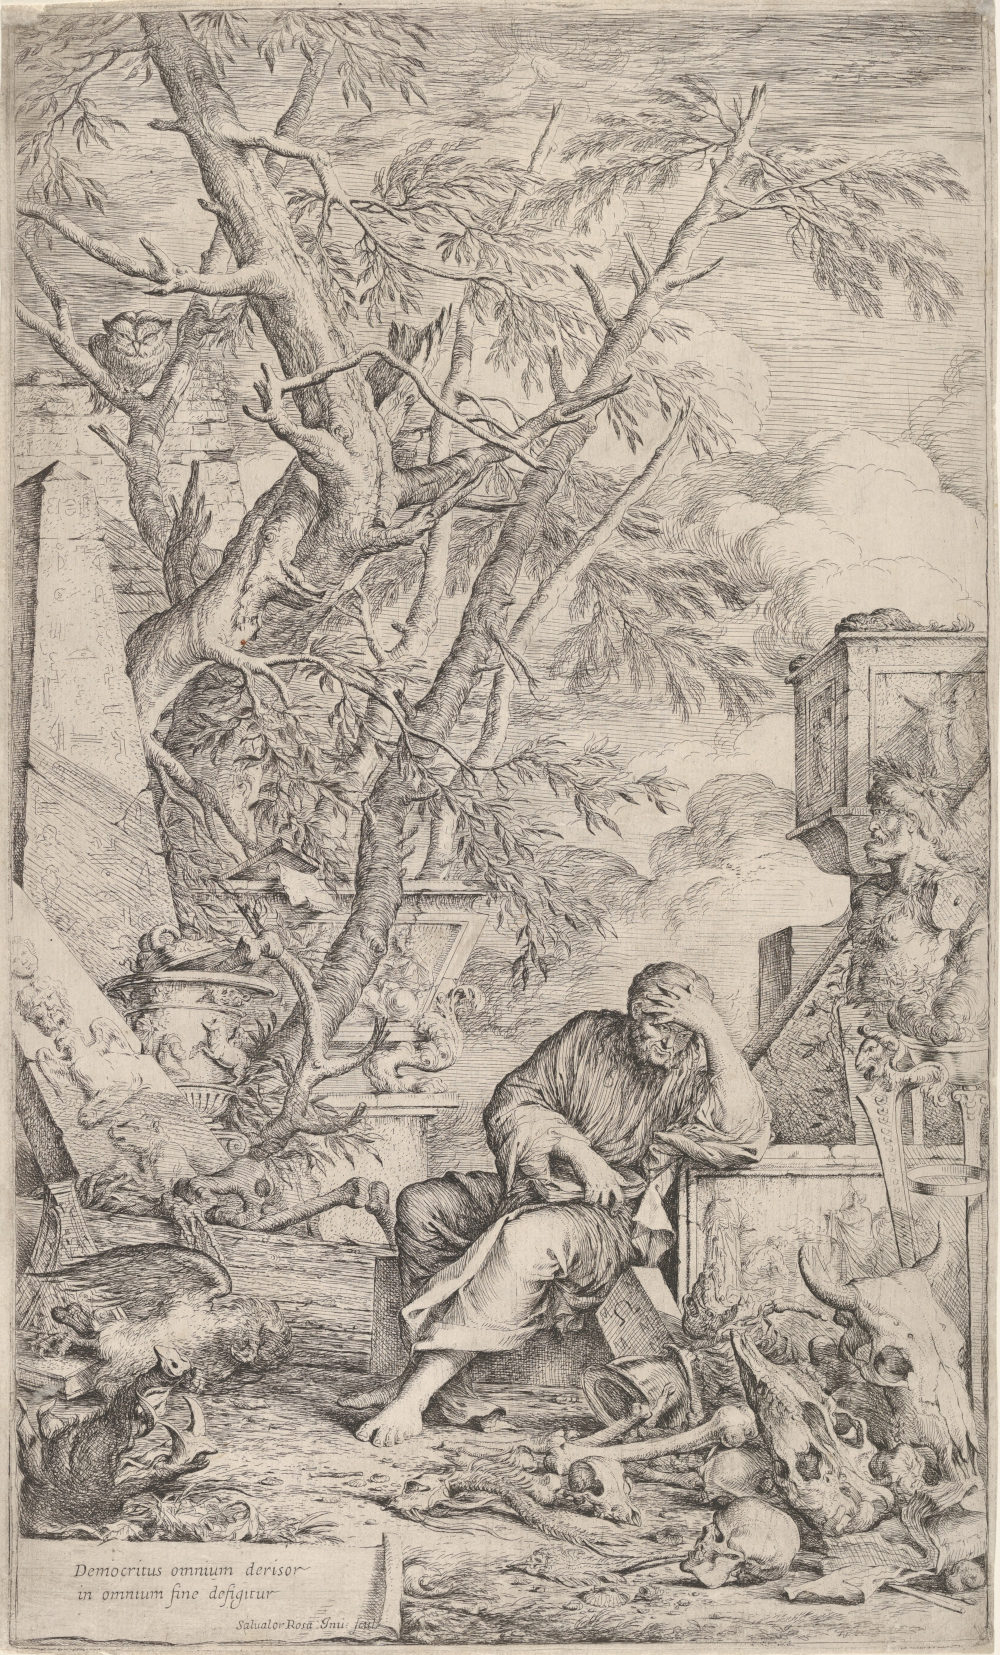
\includegraphics[keepaspectratio,width=0.9\textwidth]{Democritus-in-MeditationDP831915-small.jpg}
  \captionart{DemocritusinMeditation}
  \label{fig:democritusinmeditation}
\end{figure}
% Force float here
\clearpage{}
}
